% =============================================================================
% EpiForecast-MX — Avance 5: Modelo Final (Ensemble Learning)
% Equipo 01 — Maestría en Inteligencia Artificial Aplicada (MNA)
% Tecnológico de Monterrey x Instituto Mexicano del Seguro Social
% =============================================================================
\documentclass[12pt, letterpaper]{article}

% -- Paquetes ----------------------------------------------------------------
\usepackage[utf8]{inputenc}
\usepackage[T1]{fontenc}
\usepackage[spanish,es-tabla]{babel}
\usepackage{geometry}
\geometry{letterpaper, margin=2.5cm, top=3cm, bottom=2.5cm}
\usepackage{graphicx}
\usepackage{float}
\usepackage{booktabs}
\usepackage{tabularx}
\usepackage{longtable}
\usepackage{multirow}
\usepackage{xcolor}
\usepackage{colortbl}
\usepackage{fancyhdr}
\usepackage{titlesec}
\usepackage{enumitem}
\usepackage{amsmath, amssymb}
\usepackage{caption}
\usepackage{subcaption}
\usepackage[most]{tcolorbox}
\usepackage{fontawesome5}
\usepackage{pifont}
\usepackage{parskip}
\usepackage{setspace}
\usepackage{array}
\usepackage[bottom]{footmisc}
\usepackage{xurl}          % URLs con salto de línea automático
\usepackage[breaklinks=true]{hyperref}

% -- Colores institucionales IMSS / EpiForecast ------------------------------
\definecolor{burgundy}{HTML}{9B2242}
\definecolor{darkburgundy}{HTML}{6F1D46}
\definecolor{teal}{HTML}{00524E}
\definecolor{darkteal}{HTML}{173F35}
\definecolor{gold}{HTML}{B58500}
\definecolor{coolgray}{HTML}{97999B}
\definecolor{imssblue}{HTML}{003A70}
\definecolor{cream}{HTML}{F5EDE0}
\definecolor{lightgreen}{HTML}{E6F4EA}
\definecolor{lightyellow}{HTML}{FEF7E0}
\definecolor{lightred}{HTML}{FDE8E8}

% Colores específicos por Motor MLOps
\definecolor{cprophet}{HTML}{004D40}
\definecolor{cdeepar}{HTML}{880E4F}
\definecolor{censemble}{HTML}{FF6F00}
\definecolor{cstacking}{HTML}{1A237E}

% -- Configuración de hyperref -----------------------------------------------
\hypersetup{
    colorlinks=true,
    linkcolor=teal,
    citecolor=burgundy,
    urlcolor=imssblue,
    bookmarksopen=true,
    pdftitle={EpiForecast-MX | Avance 5: Modelo Final},
    pdfauthor={Equipo 01 | MNA Tec de Monterrey},
}

% -- Pies de foto centrados y en gris ----------------------------------------
\captionsetup{
    font={small, color=coolgray},
    labelfont={bf, color=coolgray},
    justification=centering
}
\captionsetup[subfigure]{
    font={small, color=coolgray},
    labelfont={bf, color=coolgray},
    justification=centering
}

% -- Headers y footers -------------------------------------------------------
\pagestyle{fancy}
\fancyhf{}
\fancyhead[L]{\small\textcolor{coolgray}{EpiForecast-MX | Avance 5: Modelo Final}}
\fancyhead[R]{\small\textcolor{coolgray}{Equipo 01 | MNA | Tec de Monterrey}}
\fancyfoot[C]{\thepage}
\fancyfoot[R]{\small\textcolor{coolgray}{Marzo 2026}}
\renewcommand{\headrulewidth}{0.4pt}
\renewcommand{\footrulewidth}{0.2pt}

% -- Títulos con colores IMSS ------------------------------------------------
\titleformat{\section}
  {\Large\bfseries\color{teal}}{\thesection.}{0.5em}{}[\vspace{-0.5em}\textcolor{teal}{\rule{\textwidth}{1pt}}]
\titleformat{\subsection}
  {\large\bfseries\color{burgundy}}{\thesubsection}{0.5em}{}
\titleformat{\subsubsection}
  {\normalsize\bfseries\color{darkteal}}{\thesubsubsection}{0.5em}{}

% -- Cajas de callout --------------------------------------------------------
\newtcolorbox{insightbox}[1][]{
  colback=lightgreen, colframe=teal,
  boxrule=0pt, leftrule=4pt, arc=2pt,
  fonttitle=\bfseries, title=#1
}
\newtcolorbox{warningbox}[1][]{
  colback=lightyellow, colframe=gold,
  boxrule=0pt, leftrule=4pt, arc=2pt,
  fonttitle=\bfseries, title=#1
}
\newtcolorbox{criticalbox}[1][]{
  colback=lightred, colframe=burgundy,
  boxrule=0pt, leftrule=4pt, arc=2pt,
  fonttitle=\bfseries, title=#1
}

% Caja de Campeón en Producción (Dorada)
\newtcolorbox{championbox}[1][]{
  colback=white, colframe=gold,
  boxrule=2pt, arc=6pt,
  fonttitle=\bfseries\large, coltitle=black,
  title={\textcolor{gold}{\faTrophy}\ \textbf{Modelo Campeón en Producción} #1}
}

% -- Comandos personalizados -------------------------------------------------
\newcommand{\smape}{\textsc{smape}}
\newcommand{\mase}{\textsc{mase}}
\newcommand{\rmse}{\textsc{rmse}}
\newcommand{\imss}{\textsc{imss}}
\newcommand{\tabref}[1]{Tabla~\ref{#1}}
\newcommand{\figref}[1]{Figura~\ref{#1}}
\newcommand{\secref}[1]{Sección~\ref{#1}}

\begin{document}

% =============================================================================
% PORTADA
% =============================================================================
\begin{titlepage}
\begin{center}

\vspace*{0.5cm}

% Logos institucionales (subir a Overleaf: logo_tec.png y logo_imss.png)

\includegraphics[height=2cm]{logo_tec.png}\hspace{2cm}
\includegraphics[height=2.5cm]{logo_imss.png}

\vspace{0.5cm}

{\small Instituto Tecnológico y de Estudios Superiores de Monterrey}\\[0.1cm]
{\small Maestría en Inteligencia Artificial Aplicada (MNA)}\\[0.5cm]

\textcolor{teal}{\rule{\textwidth}{2pt}}\\[0.4cm]
{\Huge\bfseries\textcolor{teal}{EpiForecast-MX}}\\[0.2cm]
{\LARGE\textcolor{burgundy}{Avance 5: Modelo Final (Ensemble Learning)}}\\[0.3cm]
\textcolor{teal}{\rule{\textwidth}{2pt}}\\[0.8cm]

{\large\textit{Generalización de modelos nacionales de pronóstico epidemiológico\\hacia un enfoque modular con desagregación por sexo y\\entidad federativa en México}}\\[1.2cm]

{\large\textbf{Materia:} Proyecto Integrador | TC5035.10}\\[0.5cm]

\begin{tabular}{ll}
\textbf{Asesora:}     & Dra.\ Grettel Barceló Alonso \\
\textbf{Director MNA:}& Dr.\ Luis Eduardo Falcón Morales \\
\textbf{Profesora:}   & Mtra.\ Verónica Sandra Guzmán de Valle \\
\textbf{IMSS:}        & Dra.\ Ruth Pérez-Hernández (Líder de Proyecto) \\
                      & Dra.\ Lina Díaz Castro (Investigadora en Psiquiatría) \\
\end{tabular}\\[1cm]

\textbf{\Large Equipo 01}\\[0.4cm]
\begin{tabular}{lll}
\textbf{Javier A. Rebull Saucedo} & A01795838 & Sr.\ Assoc.\ Dev., Santander Bank US \\
\textbf{Juan Carlos Pérez Nava}   & A01795941 & Head of Area, IMSS \\
\textbf{Luis G. Sánchez Salazar}  & A01232963 & Sr.\ Controls Engineer, Tesla \\
\end{tabular}\\[1.0cm]

{\large Marzo 2026}

\end{center}
\end{titlepage}

% =============================================================================
% TABLA DE CONTENIDOS
% =============================================================================
\newpage
\tableofcontents
\newpage

% =============================================================================
% ECOSISTEMA WEB DEL PROYECTO
% =============================================================================
\section{Ecosistema Web del Proyecto}\label{sec:ecosistema}

El proyecto EpiForecast-MX cuenta con un ecosistema completo de herramientas web para la exploración interactiva de resultados. \textbf{Se recomienda consultar estos recursos en línea para obtener la experiencia completa} con visualizaciones interactivas, filtros dinámicos y datos en tiempo real.

\begin{table}[H]
\centering
\caption{Recursos web del proyecto EpiForecast-MX}
\label{tab:enlaces}
\scriptsize
\setlength{\tabcolsep}{4pt}
\begin{tabularx}{\textwidth}{>{\bfseries}l X l}
\toprule
\textbf{Recurso} & \textbf{Descripción} & \textbf{Enlace} \\
\midrule
Repositorio GitHub & Código fuente, pipelines, datos y documentación & \href{https://github.com/IntegradorIMSS2026Team01/EpiForecast-MX}{GitHub} \\
Página Web & Portal central del proyecto & \href{https://proyectointegrador.org}{proyectointegrador.org} \\
Dashboard Tableau & Visualización interactiva de incidencia y pronósticos & \href{https://proyectointegrador.org/epidashboard}{/epidashboard} \\
Pronósticos & Gráficos de predicción a máximo detalle & \href{https://proyectointegrador.org/reports/}{/reports} \\
Resultados & Métricas, comparativas y análisis de rendimiento & \href{https://proyectointegrador.org/reporte_resultados}{/reporte\_resultados} \\
Bitácora v1$\to$v6 & Recorrido completo de iteraciones Prophet & \href{https://proyectointegrador.org/bitacora_modelado}{/bitacora\_modelado} \\
Batalla de Modelos & 6 algoritmos $\cdot$ 258 series $\cdot$ 1,548 trials en SageMaker & \href{https://proyectointegrador.org/comparacion_modelos}{/comparacion\_modelos} \\
Ficha Técnica & Anatomía completa del modelo Prophet & \href{https://proyectointegrador.org/ficha_tecnica_prophet}{/ficha\_tecnica\_prophet} \\
Hiperparámetros & Palancas de ajuste y su impacto en el pronóstico & \href{https://proyectointegrador.org/hiperparametros_modelos}{/hiperparametros} \\
Dashboard Build & Del dato crudo a Tableau Public & \href{https://proyectointegrador.org/construccion_dashboard}{/construccion\_dashboard} \\
Conclusiones & Hallazgos principales y próximos pasos & \href{https://proyectointegrador.org/conclusiones}{/conclusiones} \\
Referencias & Fuentes académicas y técnicas & \href{https://proyectointegrador.org/referencias}{/referencias} \\
\bottomrule
\end{tabularx}
\end{table}

% =============================================================================
% CONTEXTO DEL PROYECTO
% =============================================================================
\section{Contexto del Proyecto}\label{sec:contexto}

\subsection{Problema y motivación}

El Instituto Mexicano del Seguro Social (\imss{}) atiende a más de 80 millones de derechohabientes y requiere pronósticos epidemiológicos confiables para la planificación estratégica de recursos médicos. Actualmente, la planeación de insumos para padecimientos neurológicos y de salud mental se basa en promedios históricos, sin capacidad de anticipar cambios de tendencia.

EpiForecast-MX desarrolla un sistema de pronóstico para tres padecimientos CIE-10 (Clasificación Internacional de Enfermedades, 10.ª revisión):
\begin{itemize}[noitemsep]
    \item \textbf{Depresión (F32)} --- La de mayor incidencia y variabilidad, fuertemente impactada por COVID-19.
    \item \textbf{Enfermedad de Parkinson (G20)} --- Baja incidencia con patrones regulares.
    \item \textbf{Enfermedad de Alzheimer (G30)} --- Incidencia baja y estable; la más predecible.
\end{itemize}

Los datos provienen de los Boletines Epidemiológicos Semanales del SINAVE (Sistema Nacional de Vigilancia Epidemiológica), procesados y convertidos a tasas por 100,000 habitantes usando proyecciones de población del INEGI. El sistema cubre las \textbf{32 entidades federativas} con desagregación por \textbf{sexo} (general, hombres, mujeres), generando \textbf{333 series de producción}: 288 estatales + 36 regionales + 9 nacionales (es decir, 3 padecimientos $\times$ 37 geografías $\times$ 3 cortes demográficos). Los modelos regionales actúan como fallback (respaldo) cuando la serie estatal tiene datos insuficientes.

\subsection{Datos y periodo de estudio}

\begin{table}[H]
\centering
\caption{Características del dataset}
\label{tab:dataset}
\scriptsize
\setlength{\tabcolsep}{4pt}
\begin{tabular}{ll}
\toprule
\textbf{Característica} & \textbf{Valor} \\
\midrule
Fuente primaria        & Boletines SINAVE (PDF $\to$ scraping automatizado) \\
Fuente demográfica     & Proyecciones INEGI \\
Periodo                & 2014 -- 2026 (actualización semanal) \\
Frecuencia             & Semanal (52--53 semanas/año) \\
Registros totales      & $\approx$60,288 \\
Unidad                 & Tasa por 100,000 habitantes \\
Series de producción   & 288 estatales + 36 regionales + 9 nacionales = \textbf{333} \\
Motores evaluados      & 4 (Prophet, DeepAR, Ensemble, Stacking) $\times$ 333 = 1,332 \\
Series benchmarked     & 258 en SageMaker (39 omitidas por varianza $<$ 0.5) \\
\bottomrule
\end{tabular}
\end{table}

% =============================================================================
% SECCIONES MODIFICADAS PARA INSERTAR EN EL LATEX DE AVANCE 5
% =============================================================================
%
% INSTRUCCIONES DE INTEGRACIÓN:
%
% 1) En la Sección 2.2 "Datos y periodo de estudio", DESPUÉS de la tabla
%    \label{tab:dataset} y ANTES del \newpage, insertar las dos tablas
%    y el texto que aparecen abajo (Tabla de Composición + Tabla de Regiones).
%
% 2) Opcionalmente, en la Sección 6.1 ya existe la tabla tab:dist_prod;
%    se puede agregar una referencia cruzada al nuevo desglose.
%
% =============================================================================


% ---- INSERTAR DESPUÉS DE \end{table} de tab:dataset -----------------------

\subsubsection*{Composición de las 333 Series de Producción}

Para asegurar la trazabilidad del sistema, es fundamental entender cómo se obtiene el número \textbf{333} de series de producción. La fórmula es directa:

\begin{equation}
\underbrace{37}_{\text{geografías}} \;\times\; \underbrace{3}_{\text{padecimientos}} \;\times\; \underbrace{3}_{\text{cortes demográficos}} \;=\; \mathbf{333} \text{ series}
\end{equation}

La \tabref{tab:composicion333} desglosa cada nivel geográfico:

\begin{table}[H]
\centering
\caption{Desglose de las 333 series de producción por nivel geográfico}
\label{tab:composicion333}
\small
\begin{tabular}{l c c c r}
\toprule
\textbf{Nivel geográfico} & \textbf{Geografías} & \textbf{$\times$ Padecimientos} & \textbf{$\times$ Modos} & \textbf{= Modelos} \\
\midrule
\rowcolor{lightgreen!15}
Estatal             & 32 entidades federativas & 3 & 3 & \textbf{288} \\
Regional (fallback) & 4 regiones INEGI         & 3 & 3 & \textbf{36}  \\
Nacional            & 1 (país completo)        & 3 & 3 & \textbf{9}   \\
\midrule
\textbf{Total}      & \textbf{37}              &   &   & \textbf{333} \\
\bottomrule
\end{tabular}
\vspace{0.2cm}

{\scriptsize
\textbf{Padecimientos:} Depresión (F32), Parkinson (G20), Alzheimer (G30). \\
\textbf{Modos demográficos:} General (ambos sexos), Hombres, Mujeres. \\
\textbf{Nota:} Los 4 motores (Prophet, DeepAR, Ensemble, Stacking) compiten por cada serie, generando $4 \times 333 = 1{,}332$ evaluaciones, pero solo el ganador de cada serie pasa a producción.
}
\end{table}

\subsubsection*{Regiones INEGI de Salud Mental (Fallback)}

Los modelos regionales actúan como \textbf{respaldo (fallback)} cuando una serie estatal tiene incidencia insuficiente ($<$5 casos en 52 semanas). Las 4 regiones agrupan a los 32 estados según patrones sociodemográficos definidos por el INEGI:

\begin{table}[H]
\centering
\caption{Clasificación regional INEGI para modelos de fallback}
\label{tab:regiones_inegi}
\small
\setlength{\tabcolsep}{4pt}
\begin{tabularx}{\textwidth}{>{\bfseries}l c X}
\toprule
\textbf{Región} & \textbf{Estados} & \textbf{Entidades que la componen} \\
\midrule
\rowcolor{lightgreen!15}
Metropolitana Alta & 4 & Ciudad de México, Jalisco, Estado de México, Nuevo León \\
\addlinespace
Urbana Media & 15 & Aguascalientes, Baja California, Baja California Sur, Chihuahua, Coahuila, Colima, Durango, Guanajuato, Morelos, Querétaro, San Luis Potosí, Sinaloa, Sonora, Tamaulipas, Zacatecas \\
\addlinespace
\rowcolor{lightgreen!15}
Rural / Dispersa & 7 & Guerrero, Hidalgo, Michoacán, Nayarit, Puebla, Tlaxcala, Veracruz \\
\addlinespace
Sur-Sureste Vulnerable & 6 & Campeche, Chiapas, Oaxaca, Quintana Roo, Tabasco, Yucatán \\
\midrule
\textbf{Total} & \textbf{32} & \\
\bottomrule
\end{tabularx}
\vspace{0.2cm}

{\scriptsize \textbf{Criterio de activación del fallback:} Si una serie estatal registra $<$5 casos acumulados en las últimas 52 semanas, el sistema reasigna automáticamente al modelo de su región INEGI. En producción, \textbf{8 de 333 series} requirieron este mecanismo (7 de Alzheimer y 1 de Parkinson en Campeche).}
\end{table}

\begin{insightbox}[¿Por qué 333 y no 288?]
Los \textbf{288 modelos estatales} (32 estados $\times$ 3 padecimientos $\times$ 3 modos) constituyen el núcleo del sistema. Sin embargo, agregar los \textbf{36 modelos regionales} y los \textbf{9 nacionales} cumple dos funciones críticas:
\begin{itemize}[noitemsep]
    \item \textbf{Cobertura del 100\,\%:} Las regiones INEGI actúan como red de seguridad para estados con datos insuficientes (cold start), garantizando que ninguna entidad quede sin pronóstico.
    \item \textbf{Planificación multinivel:} El IMSS requiere pronósticos no solo a nivel estatal, sino también agregados regionales y nacionales para la asignación presupuestal y logística de insumos a gran escala.
\end{itemize}
\end{insightbox}

\newpage


% =============================================================================
% 1. INTRODUCCIÓN Y RESPUESTA A RETROALIMENTACIÓN
% =============================================================================
\section{Introducción y Acciones Correctivas}\label{sec:intro}

El presente documento detalla la consolidación algorítmica del ecosistema \textbf{EpiForecast-MX} (Avance~5). En cumplimiento de los Objetivos de esta entrega, el sistema evoluciona desde modelos \textit{baseline} individuales hacia un framework completo de \textbf{Ensemble Learning} (técnica que combina múltiples modelos para obtener predicciones más robustas) con estrategias homogéneas y heterogéneas, evaluando un total de \textbf{1,332 modelos} (4 motores $\times$ 333 combinaciones clínicas) sobre \textbf{630 semanas} de datos históricos (2014--2026) para potenciar la precisión clínica en el Instituto Mexicano del Seguro Social (\imss{}).

El sistema pronostica la incidencia semanal (es decir, cuántos casos nuevos se esperan cada semana) de tres padecimientos neurológicos y psiquiátricos: \textbf{Depresión (F32)}, \textbf{Parkinson (G20)} y \textbf{Alzheimer (G30)}, para las \textbf{32 entidades federativas}, desagregados por sexo (masculino, femenino y el consolidado de ambos), con un horizonte de \textbf{52 semanas}.

\begin{insightbox}[Crónica del Avance 5]
La semana de cierre del Avance~5 fue, sin duda, la más exigente del proyecto. Entrenar \textbf{1,332 modelos} no es una cifra retórica: representó ciclos de entrenamiento que superaban las \textbf{13 horas continuas}, sesiones de depuración que se extendían hasta la madrugada y la frustración de descubrir tras horas de cómputo que un bug sutil en el preprocesamiento invalidaba una corrida completa. Hubo noches en que los tres integrantes del equipo trabajamos en paralelo desde tres zonas horarias distintas, coordinando entrenamientos en AWS SageMaker mientras se ejecutaban validaciones locales en laptops a su máxima capacidad.

Detectar la fuga de datos en el feature builder, corregirla y volver a entrenar los 333 modelos del Ensemble significó perder un día completo de trabajo. La convergencia fallida del ElasticNet en series de ceros nos obligó a diseñar 7 capas de defensa en una sola noche. DeepAR requirió múltiples intentos de backtest con ventana expansiva antes de producir métricas honestas.

Sin embargo, cada obstáculo superado consolidó algo más profundo que un modelo: \textbf{la convicción de que la ciencia de datos puede transformar la salud pública de México}. Ver que DeepAR alcanzaba un SMAPE del \textbf{7.49\,\%} en Depresión es decir, que podemos predecir con más del 92\,\% de precisión cuántos pacientes con depresión atenderá cada estado la próxima semana justificó cada hora invertida. Saber que estos pronósticos llegarán al escritorio de tomadores de decisión del \imss{} para planificar camas, insumos y personal para padecimientos que afectan a millones de mexicanos convirtió el agotamiento en orgullo.
\end{insightbox}

A partir de la retroalimentación provista por la Dra.\ Grettel Barceló en el avance anterior, el equipo implementó mejoras estructurales críticas:

\begin{table}[H]
\centering
\caption{Atención a la retroalimentación y acciones correctivas implementadas}
\label{tab:feedback}
\small
\begin{tabularx}{\textwidth}{>{\bfseries\hsize=.35\hsize}X >{\hsize=.65\hsize}X}
\toprule
Comentario / Hallazgo & Resolución MLOps Implementada \\
\midrule
\rowcolor{lightgreen!20}
Aclarar el origen de los 312 (ahora 333) modelos base. & \textcolor{teal}{\ding{51}} \textbf{Matemática de la red:} (32 estados + 4 regiones fallback + 1 nacional) $\times$ 3 cortes demográficos = \textbf{111 series por padecimiento} $\times$ 3 padecimientos = \textbf{333 series totales}. Al competir 4 motores (Prophet, DeepAR, Ensemble, Stacking), el sistema evalúa $4 \times 333 = 1{,}332$ combinaciones, pero en producción se inyectan estrictamente \textbf{333 modelos ganadores} (el mejor motor por serie). \\
\addlinespace
Reemplazar MAPE por SMAPE debido a la inflación por ceros. & \textcolor{teal}{\ding{51}} \textbf{SMAPE como métrica primaria}~[6,\,7]: SMAPE $= \frac{2|y - \hat{y}|}{|y| + |\hat{y}|}$ penaliza de forma simétrica y no se infla al infinito con los ceros de Alzheimer y Parkinson. Es la métrica de selección automática en producción. \\
\addlinespace
\rowcolor{lightgreen!20}
Prophet se ve plano fuera de pandemia. Faltan picos. & \textcolor{teal}{\ding{51}} \textbf{Diversificación algorítmica:} Prophet es propenso al suavizado lineal. Con \textbf{DeepAR} (LSTM) y \textbf{Ensemble con XGBoost}, el sistema captura la varianza de corto plazo y los picos estacionales reales. \\
\addlinespace
El Dashboard muestra Casos Absolutos en vez de Tasas. & \textcolor{teal}{\ding{51}} \textbf{Diseño clínico deliberado:} El sistema entrena internamente con tasas (por 100k hab.) para aislar la demografía. Al predecir, \textbf{desnormaliza} multiplicando por población. Tableau muestra \textbf{casos absolutos} porque el IMSS planea camas e insumos con pacientes, no con tasas. \\
\addlinespace
\rowcolor{lightgreen!20}
Separar niveles territoriales en los filtros de la UI. & \textcolor{teal}{\ding{51}} \textbf{Refactorización UI:} Tableau ahora muestra las 32 entidades en un combo independiente. Las regiones INEGI y la vista nacional tienen vistas separadas. \\
\addlinespace
Frecuencia de re-entrenamiento. & \textcolor{teal}{\ding{51}} \textbf{Política de Producción:} Pronósticos a \textbf{52 semanas}, con re-entrenamiento paramétrico programado de forma \textbf{trimestral}. \\
\bottomrule
\end{tabularx}
\end{table}

\newpage

% =============================================================================
% 2. MARCO TEÓRICO Y DISEÑO DE ENSAMBLES
% =============================================================================
\section{Marco Teórico y Diseño de Ensambles}\label{sec:marco}

\subsection{Filosofía del Ensemble Learning}
El aprendizaje por ensamble (\textit{Ensemble Learning}) combina múltiples aprendices base para producir un pronóstico superior y más generalizable~[1]. En series de tiempo epidemiológicas, donde la varianza interestatal es alta y el impacto del COVID-19 generó rupturas de régimen, un modelo individual suele caer en el dilema de sesgo-varianza~[2].

Para EpiForecast-MX, diseñamos una batería de motores que ataca ambos frentes: técnicas de \textbf{redes multi-serie} para estabilizar la varianza y \textbf{Boosting/Stacking} para reducir el sesgo.

\subsection{Arquitectura de los 4 Motores de Pronóstico}

El sistema pone a competir 4 arquitecturas radicalmente distintas (\tabref{tab:motores}):

\begin{table}[H]
\centering
\caption{Arquitectura de los 4 Motores de Pronóstico}
\label{tab:motores}
\small
\begin{tabularx}{\textwidth}{>{\raggedright\arraybackslash}p{1.8cm} >{\raggedright\arraybackslash}p{2.2cm} X}
\toprule
\textbf{Motor} & \textbf{Estrategia} & \textbf{Descripción Técnica} \\
\midrule
\rowcolor{cprophet!10}
\textbf{Prophet} & Baseline individual & Modelo aditivo bayesiano (Meta/Facebook)~[4]. Descomposición: tendencia (logística segmentada con 12--25 \textit{changepoints}) + estacionalidad anual (series de Fourier, orden 10) + regresores (holiday COVID: 913 días). Validación cruzada con 4 folds temporales y pesos progresivos $[0.5, 0.75, 1.0, 1.25]$. Aplica $\log(1+y)$ y normaliza a tasa por 100k habitantes. \\
\addlinespace
\rowcolor{cdeepar!10}
\textbf{DeepAR} & Ensamble homogéneo (multi-serie) & Red neuronal LSTM autoregresiva probabilística~[3]. Implementada sobre GluonTS + PyTorch. Entrena las 32 series estatales \textbf{simultáneamente}, aprendiendo correlaciones espaciales vía \textit{transfer learning}. Arquitectura: 2 capas LSTM, 80 celdas, dropout 0.15, distribución Student-$t$. Contexto de 104 semanas (2 años), 200 muestras Monte Carlo para intervalos de confianza. \\
\addlinespace
\rowcolor{censemble!10}
\textbf{Ensemble} & Heterogéneo paralelo & Combina la tendencia estacional de \textbf{Prophet}~[4] con la corrección de \textbf{XGBoost}~[5] alimentado con 20 \textit{features} temporales (7 lags, 5 medias móviles, tasa de cambio, cíclicos seno/coseno, flag COVID). Los pesos se aprenden vía regresión \textbf{Ridge} sobre predicciones Out-of-Fold (4 folds, ventana expansiva). Grid search de 36 combinaciones. \\
\addlinespace
\rowcolor{cstacking!10}
\textbf{Stacking} & Heterogéneo generalizado & Une a 3 expertos independientes: \textbf{Prophet}~[4], \textbf{ETS} (Holt-Winters~[10], período 52) y \textbf{LightGBM}~[8] (300 árboles, profundidad 4). El meta-learner \textbf{ElasticNet}~[9] ($\alpha=1.0$, $L_1$-ratio$=0.5$, pesos $\geq 0$) inyecta variables $\sin(2\pi w/52)$ y $\cos(2\pi w/52)$ para decidir en qué época del año confiar más en cada experto. \\
\bottomrule
\end{tabularx}
\end{table}

\begin{insightbox}[Hallazgo Empírico: El Paradigma Macro vs.\ Micro]
Se comprobó empíricamente una ley matemática en el sistema:
\begin{itemize}[noitemsep]
    \item A nivel \textbf{Micro} (estatal, alta varianza, series de 0--5 casos/semana), \textbf{DeepAR} gana abrumadoramente al ``tomar prestada'' información espacial de otros estados. Gana en el \textbf{97.3\,\%} de las series de Depresión y \textbf{83.8\,\%} de Parkinson.
    \item A nivel \textbf{Macro} (Nacional, señal suavizada por la Ley de los Grandes Números), los meta-modelos heterogéneos (\textbf{Ensemble y Stacking}) exprimen mayor precisión al combinar lógicas lineales con árboles de decisión.
\end{itemize}
\end{insightbox}

\newpage

% =============================================================================
% 3. DESAFÍOS TÉCNICOS Y LECCIONES APRENDIDAS
% =============================================================================
\section{Desafíos Técnicos y Lecciones Aprendidas}\label{sec:desafios}

El camino hacia los 1,332 modelos no fue lineal. A continuación se documentan los obstáculos técnicos más significativos y las soluciones de ingeniería que el equipo diseñó para superarlos.

\subsection{El Fantasma del Data Leakage en DeepAR}\label{subsec:leakage}

\begin{criticalbox}[Alerta Crítica: Detección y Eliminación de Fuga de Datos]
Durante la auditoría de calidad, el equipo descubrió que \textit{GluonTS} (el backend de DeepAR) \textbf{no genera fitted values históricos de forma nativa}. Ante su ausencia, el pipeline original copiaba los valores reales ($y$) como predicción ($\hat{y}$), produciendo un \smape{} \textit{in-sample} del \textbf{0\,\%}: una falsa perfección que habría invalidado cualquier diagnóstico de overfitting entregado al \imss{}.
\end{criticalbox}

\textbf{Solución: Backtest por Ventana Expansiva (\textit{Expanding-Window}).} Se programó un procedimiento estricto de retrovalidación. A partir de la semana 53, el motor retrocede en el tiempo, bloquea su conocimiento del futuro y realiza inferencias en bloques del tamaño del horizonte (52 semanas). Para la variante multi-serie (32 estados simultáneos), donde un \textit{backtest} completo por ventana expansiva habría requerido $32 \times N$ pasadas de GPU, se implementó una estrategia híbrida: valores reales para la mayor parte del historial y un único paso de \textit{backtest} honesto sobre las últimas 52 semanas de entrenamiento.

El costo computacional se incrementó significativamente (de $\sim$1 hora a $\sim$4 horas en macOS M3, o $\sim$1.5 horas en AWS SageMaker con GPU NVIDIA T4), pero aseguró que el diagnóstico entregado al \imss{} sea \textbf{estadísticamente honesto} y que las bandas de confianza reflejen incertidumbre real, no ruido de entrenamiento.

\subsection{El Cold Start de DeepAR en Series de Bajo Volumen}\label{subsec:coldstart}

\begin{warningbox}[Cold Start: Cuando la Red Neuronal No Tiene Suficiente Señal]
Las series de \textbf{Alzheimer (G30)} representan el peor escenario para una red neuronal: estados como Baja California Sur, Tlaxcala o Campeche registran \textbf{0--2 casos por semana}. Con 630 semanas de historial donde el 60\,\% son ceros, la LSTM enfrenta un problema clásico de \textit{cold start}: la señal estadística es insuficiente para que los gradientes converjan de forma significativa.
\end{warningbox}

\textbf{Solución: Modelado Híbrido con Fallback Regional.}
\begin{enumerate}[noitemsep]
    \item Las series con incidencia $<5$ casos en 52 semanas se detectan automáticamente.
    \item Se reasignan al modelo de su \textbf{región INEGI} (Metropolitana, Urbana, Sur-Sureste o Rural), que agrega la señal de múltiples estados.
    \item En producción, \textbf{8 de las 333 series} requirieron este fallback (7 de Alzheimer y 1 de Parkinson en Campeche).
\end{enumerate}

Esto asegura cobertura del 100\,\% sin forzar modelos estadísticamente frágiles sobre datos insuficientes.

\subsection{La Convergencia Fallida del ElasticNet (Stacking)}\label{subsec:convergence}

\begin{criticalbox}[Bug Crítico: ElasticNet Muere en Series de Ceros]
Al entrenar el Stacking sobre series de Alzheimer (bajo volumen, mayoría ceros), el meta-learner \textbf{ElasticNet} lanzaba \texttt{ConvergenceWarning} y el proceso moría con \textit{leaked semaphores} de \texttt{joblib/loky}. El problema: los folds Out-of-Fold producían vectores de validación casi constantes (todo ceros), donde el optimizador no encontraba gradiente.
\end{criticalbox}

\textbf{Solución de 7 capas de defensa:}
\begin{enumerate}[noitemsep]
    \item \textbf{Guardia de varianza mínima:} Si $\sigma(y_{\text{oof}}) < 10^{-8}$, asignar pesos uniformes ($1/n$) sin intentar optimizar.
    \item \textbf{Aumento de iteraciones:} De 1,000 (default) a \textbf{10,000} con tolerancia explícita ($10^{-4}$).
    \item \textbf{Filtro por fold:} Saltar folds individuales donde la validación es constante.
    \item \textbf{Captura de warnings:} Registrar en \texttt{loguru} sin abortar el pipeline.
    \item \textbf{Fallback robusto:} Si Ridge también falla, devolver pesos uniformes.
    \item \textbf{Supresión de semáforos filtrados:} Limpieza de recursos del pool de procesos.
    \item \textbf{Propagación desde config:} Los parámetros \texttt{max\_iter} y \texttt{tol} se controlan desde \texttt{stacking.yaml}.
\end{enumerate}

Tras estas 7 mitigaciones, el Stacking completa las 333 series sin excepciones.

\subsection{Fuga de Datos en el Feature Engineering del Ensemble}\label{subsec:fuga_features}

Una segunda fuente de leakage más sutil se descubrió en el preprocesamiento de datos: la función \texttt{\_ajusta\_negativos()} usaba \texttt{shift(-1)} para mirar \textbf{una semana hacia el futuro} al interpolar valores negativos. En la frontera train/test, esto contaminaba el set de entrenamiento con información del test, inflando las métricas entre un 5\,\% y un 15\,\%.

\textbf{Solución:} Se reemplazó la interpolación bidireccional por una \textbf{media móvil retrospectiva de 3 semanas} que solo usa datos pasados. Además, los features de tasa de cambio (\texttt{roc\_4} y \texttt{roc\_52}) del XGBoost se recalcularon sobre valores \textit{shifted} ($y_{t-1}$) para garantizar que ningún feature accede a $y_t$ en el momento de la predicción.

Se añadió un test unitario dedicado (\texttt{test\_roc\_no\_leakage}) que verifica matemáticamente la ausencia de fuga en cada columna del feature builder.

\newpage

% =============================================================================
% 4. OPTIMIZACIÓN DE HIPERPARÁMETROS
% =============================================================================
\section{Optimización de Hiperparámetros}\label{sec:opt}

\subsection{Prophet: Validación Cruzada Temporal Ponderada}

Se evaluaron entre 6 y 24 combinaciones de hiperparámetros por padecimiento mediante \textbf{TimeSeriesSplit} con 4 folds temporales (test de 53 semanas cada uno). Los folds recientes reciben mayor peso $[0.5, 0.75, 1.0, 1.25]$ para priorizar el comportamiento post-pandemia.

\begin{table}[H]
\centering
\caption{Distribución de hiperparámetros óptimos de Prophet (333 modelos)}
\label{tab:prophet_hp}
\small
\begin{tabular}{lcc}
\toprule
\textbf{Hiperparámetro} & \textbf{Valor más frecuente} & \textbf{Distribución} \\
\midrule
\texttt{seasonality\_mode} & multiplicative & 65.8\,\% mult / 34.2\,\% add \\
\texttt{changepoint\_prior\_scale} & 0.01 & 38.1\,\% (0.01) / 35.1\,\% (0.03) / 17.7\,\% (0.05) \\
\texttt{seasonality\_prior\_scale} & 0.10 & 32.1\,\% (0.1) / 31.2\,\% (0.05) / 17.1\,\% (0.5) \\
\bottomrule
\end{tabular}
\end{table}

El predominio de \texttt{changepoint\_prior\_scale=0.01} (regularización fuerte) indica que las series epidemiológicas del IMSS requieren tendencias suaves: los picos son estacionales, no cambios de régimen.

\subsection{DeepAR: Arquitectura LSTM Multi-Serie}

\begin{table}[H]
\centering
\caption{Configuración final de DeepAR}
\label{tab:deepar_hp}
\small
\begin{tabular}{ll|ll}
\toprule
\textbf{Parámetro} & \textbf{Valor} & \textbf{Parámetro} & \textbf{Valor} \\
\midrule
Capas LSTM          & 2              & Tasa de aprendizaje   & $5 \times 10^{-4}$ \\
Celdas por capa     & 80             & Weight decay          & $10^{-6}$ \\
Dropout             & 0.15           & Batch size            & 32 \\
Épocas (máx.)       & 300            & Distribución          & Student-$t$ \\
Early stopping      & paciencia 15   & Muestras Monte Carlo  & 200 \\
Contexto            & 104 semanas    & Predicción            & 52 semanas \\
\bottomrule
\end{tabular}
\end{table}

La distribución \textbf{Student-$t$} (en lugar de Gaussiana) le permite a DeepAR modelar colas pesadas, crítico para capturar los picos epidemiológicos post-COVID. El contexto de \textbf{104 semanas} (2 años) permite a la red observar al menos un ciclo anual completo antes de predecir.

\subsection{Ensemble: Grid Search de 36 Combinaciones}

Para el XGBoost dentro del Ensemble, se exploraron 36 combinaciones:
\texttt{max\_depth} $\in \{3,4,5\}$, \texttt{learning\_rate} $\in \{0.01, 0.03, 0.05\}$, \texttt{subsample} $\in \{0.7, 0.8\}$, \texttt{min\_child\_weight} $\in \{5, 10\}$.

\textbf{Resultado:} \texttt{max\_depth=3}, \texttt{lr=0.03}, \texttt{subsample=0.8}, \texttt{min\_child\_weight=5}. La profundidad de 3 fue crítica: con profundidad 4, el modelo mostraba sobreajuste en series de $\sim$600 observaciones.

Los pesos aprendidos vía Ridge OOF revelan un equilibrio notable:

\begin{table}[H]
\centering
\caption{Pesos del Ensemble (Prophet + XGBoost) aprendidos vía Ridge OOF}
\label{tab:ensemble_weights}
\small
\begin{tabular}{lcc}
\toprule
\textbf{Padecimiento} & $w_{\text{Prophet}}$ & $w_{\text{XGBoost}}$ \\
\midrule
Alzheimer  & 0.578 & 0.422 \\
Depresión  & 0.548 & 0.452 \\
Parkinson  & 0.489 & \textbf{0.511} \\
\midrule
\textbf{Promedio global} & 0.538 & 0.462 \\
\bottomrule
\end{tabular}
\end{table}

En Parkinson, XGBoost recibe \textbf{mayor peso que Prophet}: la alta volatilidad semanal (ciclos de 4--8 semanas) favorece al árbol de decisión sobre el suavizador bayesiano.

\subsection{Stacking: Pesos del Meta-Learner ElasticNet}

\begin{table}[H]
\centering
\caption{Pesos del Stacking (3 expertos) aprendidos vía ElasticNet OOF}
\label{tab:stacking_weights}
\small
\begin{tabular}{lccc}
\toprule
\textbf{Padecimiento} & $w_{\text{Prophet}}$ & $w_{\text{ETS}}$ & $w_{\text{LightGBM}}$ \\
\midrule
Alzheimer  & 0.231 & 0.214 & 0.185 \\
Depresión  & 0.454 & 0.273 & 0.274 \\
Parkinson  & 0.288 & \textbf{0.356} & 0.265 \\
\midrule
\textbf{Promedio global} & 0.324 & 0.281 & 0.241 \\
\bottomrule
\end{tabular}
\end{table}

Obsérvese que la suma de pesos $< 1.0$ en varios padecimientos: el ElasticNet con restricción de no-negatividad y $L_1$-ratio=0.5 \textbf{efectivamente silencia} a los expertos que aportan ruido, poniendo su peso en cero. Esto es especialmente visible en Alzheimer, donde los 3 expertos reciben pesos modestos porque ninguno domina claramente.

\newpage

% =============================================================================
% 5. EVALUACIÓN Y COMPARATIVA DE DESEMPEÑO
% =============================================================================
\section{Evaluación y Comparativa de Desempeño (Obj.\ 3.6)}\label{sec:evaluacion}

Se consolidó un \textit{benchmark} exhaustivo evaluando los \textbf{1,332 modelos}. Todas las métricas reportadas corresponden exclusivamente a datos de \textbf{test no vistos} (posterior al 1 de enero de 2025). La \tabref{tab:global} presenta la comparativa completa.

\begin{table}[H]
\centering
\caption{Comparativa completa por padecimiento (promedios sobre 111 modelos de test)}
\label{tab:global}
\small
\begin{tabular}{ll rrrr}
\toprule
\textbf{Padecimiento} & \textbf{Motor} & \textbf{SMAPE (\%)} & \textbf{MASE} & \textbf{RMSE} & \textbf{MAE} \\
\midrule
\rowcolor{lightgreen!30}
\multirow{4}{*}{\textbf{Depresión (F32)}}
  & \textbf{DeepAR}   & \textbf{7.49}  & \textbf{0.25} & \textbf{17.97} & \textbf{13.30} \\
  & Ensemble          & 27.75          & 0.93          & 32.58          & 25.09 \\
  & Stacking          & 27.97          & 0.97          & 36.13          & 28.54 \\
  & Prophet (base)    & 29.26          & 0.91          & 31.22          & 25.68 \\
\midrule
\rowcolor{lightgreen!30}
\multirow{4}{*}{\textbf{Parkinson (G20)}}
  & \textbf{DeepAR}   & \textbf{56.73} & \textbf{0.36} & \textbf{2.64}  & \textbf{1.79} \\
  & Ensemble          & 76.13          & 0.78          & 3.73           & 2.85 \\
  & Prophet (base)    & 77.73          & 0.80          & 4.08           & 3.19 \\
  & Stacking          & 87.50          & 0.78          & 3.80           & 2.89 \\
\midrule
\rowcolor{lightyellow!30}
\multirow{4}{*}{\textbf{Alzheimer (G30)}}
  & Prophet (base)    & \textbf{116.27}$^{*}$ & 0.78   & 1.42           & 1.15 \\
  & Ensemble          & 122.25                & 0.82   & 1.44           & 1.13 \\
  & DeepAR            & 125.18                & \textbf{0.45} & \textbf{0.98} & \textbf{0.63} \\
  & Stacking          & 142.83                & 0.64   & 1.44           & 1.00 \\
\midrule
\rowcolor{cream!50}
\multirow{4}{*}{\textbf{Global (333)}}
  & \textbf{DeepAR}   & \textbf{63.13} & \textbf{0.36} & \textbf{7.20}  & \textbf{5.24} \\
  & Prophet (base)    & 74.42          & 0.83          & 12.24          & 10.00 \\
  & Ensemble          & 75.38          & 0.85          & 12.58          & 9.69 \\
  & Stacking          & 86.10          & 0.80          & 13.79          & 10.81 \\
\bottomrule
\end{tabular}
\vspace{0.2cm}

{\scriptsize $^{*}$\textit{Nota sobre Alzheimer:} Prophet aparenta ganar en SMAPE (116\,\%), pero este valor está matemáticamente inflado por la abundancia de semanas con ceros. El \textbf{MASE de DeepAR (0.45)} revela la realidad clínica: la red LSTM es un 55\,\% más precisa que la predicción naïve, y domina en RMSE y MAE absolutos.}
\end{table}

\subsection{Tasa de Victoria por Métrica (333 series)}

\begin{table}[H]
\centering
\caption{Número de series donde cada motor obtiene la mejor métrica (de 333)}
\label{tab:winrate}
\small
\begin{tabular}{l rr rr rr rr}
\toprule
\textbf{Motor} & \multicolumn{2}{c}{\textbf{SMAPE}} & \multicolumn{2}{c}{\textbf{MASE}} & \multicolumn{2}{c}{\textbf{RMSE}} & \multicolumn{2}{c}{\textbf{MAE}} \\
               & \#  & \%    & \#  & \%    & \#  & \%    & \#  & \%    \\
\midrule
\rowcolor{cdeepar!8}
DeepAR         & 231 & 69.4  & 284 & 85.3  & 269 & 80.8  & 285 & 85.6  \\
Prophet        & 69  & 20.7  & 15  & 4.5   & 53  & 15.9  & 16  & 4.8   \\
Ensemble       & 28  & 8.4   & 4   & 1.2   & 6   & 1.8   & 5   & 1.5   \\
Stacking       & 5   & 1.5   & 27  & 8.1   & 5   & 1.5   & 27  & 8.1   \\
\bottomrule
\end{tabular}
\end{table}

DeepAR domina en las 4 métricas con tasas de victoria del \textbf{69--86\,\%}. Su supremacía en MASE (85.3\,\%) y MAE (85.6\,\%) confirma que la red LSTM produce los errores absolutos más bajos, especialmente en series de bajo volumen donde \textit{transfer learning} compensa la escasez de datos locales.

\subsection{Diagnósticos de Producción}

\begin{table}[H]
\centering
\caption{Diagnósticos de calidad sobre los 333 modelos de producción}
\label{tab:diagnostics}
\small
\begin{tabular}{lrl}
\toprule
\textbf{Diagnóstico} & \textbf{Resultado} & \textbf{Interpretación} \\
\midrule
Overfitting OK ($<1.3\times$)          & 328/333 (98.5\,\%) & Control de sobreajuste efectivo \\
Overfitting Moderado ($1.3$--$2.0\times$) & 1/333          & Serie de Alzheimer, bajo volumen \\
Overfitting Alto ($>2.0\times$)         & 1/333          & Monitoreada con fallback activo \\
N/D (sin datos de train)              & 3/333          & Series regionales recalculadas \\
\midrule
Leakage OK                            & 330/333 (99.1\,\%) & Sin contaminación de datos \\
Ceros Históricos ($<$0.5\,\% train)   & 3/333          & Incidencia cero en B.C.S.\ Alzheimer (legítimo) \\
\midrule
Modelo propio                          & 325/333 (97.6\,\%) & Modelo entrenado sobre la serie \\
Fallback regional                      & 8/333 (2.4\,\%)   & Reasignado por bajo volumen \\
\bottomrule
\end{tabular}
\end{table}

\newpage

% =============================================================================
% 6. SELECCIÓN DEL MODELO DE PRODUCCIÓN
% =============================================================================
\section{Selección del Modelo de Producción (333 Series)}\label{sec:seleccion}

EpiForecast-MX no impone un algoritmo estático. El sistema implementa un \textbf{enrutador de Asignación Dinámica} que evalúa los 4 motores para cada una de las 333 combinaciones y elige al ganador basándose en:

\begin{enumerate}[noitemsep]
    \item \textbf{Menor SMAPE} sobre datos de test (métrica primaria).
    \item \textbf{Desempate por MASE} cuando la diferencia de SMAPE es $<$5\,\% (prefiere $<$1.0).
    \item \textbf{Segundo desempate por RMSE} (menor error cuadrático).
\end{enumerate}

\subsection{Distribución de Modelos Ganadores}

\begin{table}[H]
\centering
\caption{Distribución de los 333 modelos de producción por motor y padecimiento}
\label{tab:dist_prod}
\small
\begin{tabular}{l rrrr r}
\toprule
\textbf{Padecimiento} & \textbf{DeepAR} & \textbf{Prophet} & \textbf{Ensemble} & \textbf{Stacking} & \textbf{Total} \\
\midrule
\rowcolor{cdeepar!8}
Depresión (F32)  & \textbf{108} & 1  & 2  & 0 & 111 \\
Parkinson (G20)  & \textbf{89}  & 10 & 12 & 0 & 111 \\
Alzheimer (G30)  & 47           & 44 & 18 & 2 & 111 \\
\midrule
\textbf{Total}   & \textbf{244 (73.3\,\%)} & 55 (16.5\,\%) & 32 (9.6\,\%) & 2 (0.6\,\%) & \textbf{333} \\
\bottomrule
\end{tabular}
\end{table}

\begin{itemize}[noitemsep]
    \item \textcolor{cdeepar}{\textbf{DeepAR:}} 244 series (\textbf{73.3\,\%}). Dominio absoluto a nivel estatal gracias al \textit{transfer learning}.
    \item \textcolor{cprophet}{\textbf{Prophet:}} 55 series (\textbf{16.5\,\%}). Prevalece en Alzheimer donde la señal suave favorece al modelo bayesiano.
    \item \textcolor{censemble}{\textbf{Ensemble:}} 32 series (\textbf{9.6\,\%}). Gana en agregados macro y series de volatilidad media.
    \item \textcolor{cstacking}{\textbf{Stacking:}} 2 series (\textbf{0.6\,\%}). Especialista en nichos donde la diversidad de expertos agrega valor.
\end{itemize}

En Depresión, DeepAR gana \textbf{108 de 111 series} (97.3\,\%): la señal es suficientemente fuerte para que la red LSTM aproveche las correlaciones espaciales entre estados. En Alzheimer, la competencia es cerrada (47 DeepAR vs.\ 44 Prophet): la escasez de casos hace que el suavizado bayesiano de Prophet compita de igual a igual con el \textit{transfer learning} neuronal.

\subsection{Padrón Completo de Producción (333 Modelos)}

La siguiente tabla presenta la \textbf{totalidad} de los 333 modelos de producción con su motor ganador, SMAPE de test y MASE. La tabla se organiza por padecimiento, agrupando nivel nacional, regional (INEGI) y estatal.

\footnotesize
\setlength{\tabcolsep}{3pt}
\begin{longtable}{l l >{\bfseries}c r r l}
\caption{Matriz Completa de Asignación Dinámica de Producción (333 modelos)} \label{tab:long_333} \\
\toprule
\textbf{Geografía} & \textbf{Sexo} & \textbf{Motor} & \textbf{SMAPE} & \textbf{MASE} & \textbf{Razón de selección} \\
\midrule
\endfirsthead

\multicolumn{6}{c}{\small\textit{(continuación de la Tabla~\ref{tab:long_333})}} \\
\toprule
\textbf{Geografía} & \textbf{Sexo} & \textbf{Motor} & \textbf{SMAPE} & \textbf{MASE} & \textbf{Razón de selección} \\
\midrule
\endhead

\midrule
\multicolumn{6}{r}{\small\textit{Continúa en la siguiente página}} \\
\endfoot

\bottomrule
\endlastfoot
\midrule
\rowcolor{cream!50} \multicolumn{6}{c}{\textbf{Depresión (F32)}} \\
\midrule
\rowcolor{lightgreen!15} \multicolumn{6}{l}{\textit{\small Nivel Nacional}} \\
Nacional & Hom & \textcolor{cprophet}{\textbf{Prophet}} & 12.64\,\% & 0.76 & Estacionalidad pura \\
Nacional & Muj & \textcolor{censemble}{\textbf{Ensemble}} & 7.11\,\% & 0.46 & Boosting volatilidad \\
Nacional & Gral & \textcolor{censemble}{\textbf{Ensemble}} & 8.75\,\% & 0.59 & Boosting volatilidad \\
\addlinespace
\rowcolor{lightgreen!15} \multicolumn{6}{l}{\textit{\small Nivel Regional (INEGI)}} \\
Metropolitana Alta & Hom & \textcolor{cdeepar}{\textbf{DeepAR}} & 12.46\,\% & 0.74 & Transfer learning \\
Metropolitana Alta & Muj & \textcolor{cdeepar}{\textbf{DeepAR}} & 13.55\,\% & 0.77 & Transfer learning \\
Metropolitana Alta & Gral & \textcolor{cdeepar}{\textbf{DeepAR}} & 9.61\,\% & 0.56 & Transfer learning \\
Rural / Dispersa & Hom & \textcolor{cdeepar}{\textbf{DeepAR}} & 9.17\,\% & 0.52 & Transfer learning \\
Rural / Dispersa & Muj & \textcolor{cdeepar}{\textbf{DeepAR}} & 6.97\,\% & 0.42 & Transfer learning \\
Rural / Dispersa & Gral & \textcolor{cdeepar}{\textbf{DeepAR}} & 7.30\,\% & 0.45 & Transfer learning \\
Sur-Sureste Vulnerable & Hom & \textcolor{cdeepar}{\textbf{DeepAR}} & 12.96\,\% & 0.75 & Transfer learning \\
Sur-Sureste Vulnerable & Muj & \textcolor{cdeepar}{\textbf{DeepAR}} & 9.11\,\% & 0.50 & Transfer learning \\
Sur-Sureste Vulnerable & Gral & \textcolor{cdeepar}{\textbf{DeepAR}} & 11.47\,\% & 0.69 & Transfer learning \\
Urbana Media & Hom & \textcolor{cdeepar}{\textbf{DeepAR}} & 9.65\,\% & 0.53 & Transfer learning \\
Urbana Media & Muj & \textcolor{cdeepar}{\textbf{DeepAR}} & 5.84\,\% & 0.32 & Transfer learning \\
Urbana Media & Gral & \textcolor{cdeepar}{\textbf{DeepAR}} & 6.85\,\% & 0.39 & Transfer learning \\
\addlinespace
\rowcolor{lightgreen!15} \multicolumn{6}{l}{\textit{\small Nivel Estatal (32 Entidades Federativas)}} \\
Aguascalientes & Hom & \textcolor{cdeepar}{\textbf{DeepAR}} & 5.19\,\% & 0.10 & Transfer learning \\
Aguascalientes & Muj & \textcolor{cdeepar}{\textbf{DeepAR}} & 2.36\,\% & 0.05 & Transfer learning \\
Aguascalientes & Gral & \textcolor{cdeepar}{\textbf{DeepAR}} & 4.03\,\% & 0.08 & Transfer learning \\
Baja California & Hom & \textcolor{cdeepar}{\textbf{DeepAR}} & 5.60\,\% & 0.16 & Transfer learning \\
Baja California & Muj & \textcolor{cdeepar}{\textbf{DeepAR}} & 3.63\,\% & 0.16 & Transfer learning \\
Baja California & Gral & \textcolor{cdeepar}{\textbf{DeepAR}} & 2.09\,\% & 0.09 & Transfer learning \\
Baja California Sur & Hom & \textcolor{cdeepar}{\textbf{DeepAR}} & 21.99\,\% & 0.09 & Transfer learning \\
Baja California Sur & Muj & \textcolor{cdeepar}{\textbf{DeepAR}} & 18.05\,\% & 0.30 & Transfer learning \\
Baja California Sur & Gral & \textcolor{cdeepar}{\textbf{DeepAR}} & 7.82\,\% & 0.12 & Transfer learning \\
Campeche & Hom & \textcolor{cdeepar}{\textbf{DeepAR}} & 12.81\,\% & 0.36 & Transfer learning \\
Campeche & Muj & \textcolor{cdeepar}{\textbf{DeepAR}} & 7.06\,\% & 0.23 & Transfer learning \\
Campeche & Gral & \textcolor{cdeepar}{\textbf{DeepAR}} & 5.92\,\% & 0.23 & Transfer learning \\
Chiapas & Hom & \textcolor{cdeepar}{\textbf{DeepAR}} & 10.84\,\% & 0.35 & Transfer learning \\
Chiapas & Muj & \textcolor{cdeepar}{\textbf{DeepAR}} & 10.74\,\% & 0.49 & Transfer learning \\
Chiapas & Gral & \textcolor{cdeepar}{\textbf{DeepAR}} & 6.39\,\% & 0.33 & Transfer learning \\
Chihuahua & Hom & \textcolor{cdeepar}{\textbf{DeepAR}} & 5.76\,\% & 0.12 & Transfer learning \\
Chihuahua & Muj & \textcolor{cdeepar}{\textbf{DeepAR}} & 2.98\,\% & 0.08 & Transfer learning \\
Chihuahua & Gral & \textcolor{cdeepar}{\textbf{DeepAR}} & 3.73\,\% & 0.10 & Transfer learning \\
Ciudad de México & Hom & \textcolor{cdeepar}{\textbf{DeepAR}} & 2.66\,\% & 0.13 & Transfer learning \\
Ciudad de México & Muj & \textcolor{cdeepar}{\textbf{DeepAR}} & 3.24\,\% & 0.16 & Transfer learning \\
Ciudad de México & Gral & \textcolor{cdeepar}{\textbf{DeepAR}} & 3.48\,\% & 0.16 & Transfer learning \\
Coahuila & Hom & \textcolor{cdeepar}{\textbf{DeepAR}} & 2.12\,\% & 0.05 & Transfer learning \\
Coahuila & Muj & \textcolor{cdeepar}{\textbf{DeepAR}} & 7.78\,\% & 0.17 & Transfer learning \\
Coahuila & Gral & \textcolor{cdeepar}{\textbf{DeepAR}} & 2.15\,\% & 0.05 & Transfer learning \\
Colima & Hom & \textcolor{cdeepar}{\textbf{DeepAR}} & 5.99\,\% & 0.25 & Transfer learning \\
Colima & Muj & \textcolor{cdeepar}{\textbf{DeepAR}} & 4.41\,\% & 0.16 & Transfer learning \\
Colima & Gral & \textcolor{cdeepar}{\textbf{DeepAR}} & 7.63\,\% & 0.30 & Transfer learning \\
Durango & Hom & \textcolor{cdeepar}{\textbf{DeepAR}} & 2.52\,\% & 0.06 & Transfer learning \\
Durango & Muj & \textcolor{cdeepar}{\textbf{DeepAR}} & 16.90\,\% & 0.46 & Transfer learning \\
Durango & Gral & \textcolor{cdeepar}{\textbf{DeepAR}} & 12.91\,\% & 0.41 & Transfer learning \\
Guanajuato & Hom & \textcolor{cdeepar}{\textbf{DeepAR}} & 3.66\,\% & 0.17 & Transfer learning \\
Guanajuato & Muj & \textcolor{cdeepar}{\textbf{DeepAR}} & 3.21\,\% & 0.11 & Transfer learning \\
Guanajuato & Gral & \textcolor{cdeepar}{\textbf{DeepAR}} & 1.94\,\% & 0.08 & Transfer learning \\
Guerrero & Hom & \textcolor{cdeepar}{\textbf{DeepAR}} & 8.21\,\% & 0.24 & Transfer learning \\
Guerrero & Muj & \textcolor{cdeepar}{\textbf{DeepAR}} & 5.07\,\% & 0.11 & Transfer learning \\
Guerrero & Gral & \textcolor{cdeepar}{\textbf{DeepAR}} & 4.22\,\% & 0.10 & Transfer learning \\
Hidalgo & Hom & \textcolor{cdeepar}{\textbf{DeepAR}} & 9.30\,\% & 0.26 & Transfer learning \\
Hidalgo & Muj & \textcolor{cdeepar}{\textbf{DeepAR}} & 9.46\,\% & 0.36 & Transfer learning \\
Hidalgo & Gral & \textcolor{cdeepar}{\textbf{DeepAR}} & 2.80\,\% & 0.11 & Transfer learning \\
Jalisco & Hom & \textcolor{cdeepar}{\textbf{DeepAR}} & 6.94\,\% & 0.34 & Transfer learning \\
Jalisco & Muj & \textcolor{cdeepar}{\textbf{DeepAR}} & 6.15\,\% & 0.26 & Transfer learning \\
Jalisco & Gral & \textcolor{cdeepar}{\textbf{DeepAR}} & 3.96\,\% & 0.18 & Transfer learning \\
Michoacán & Hom & \textcolor{cdeepar}{\textbf{DeepAR}} & 3.01\,\% & 0.11 & Transfer learning \\
Michoacán & Muj & \textcolor{cdeepar}{\textbf{DeepAR}} & 2.98\,\% & 0.11 & Transfer learning \\
Michoacán & Gral & \textcolor{cdeepar}{\textbf{DeepAR}} & 1.03\,\% & 0.05 & Transfer learning \\
Morelos & Hom & \textcolor{cdeepar}{\textbf{DeepAR}} & 2.94\,\% & 0.06 & Transfer learning \\
Morelos & Muj & \textcolor{cdeepar}{\textbf{DeepAR}} & 1.56\,\% & 0.04 & Transfer learning \\
Morelos & Gral & \textcolor{cdeepar}{\textbf{DeepAR}} & 1.40\,\% & 0.04 & Transfer learning \\
México & Hom & \textcolor{cdeepar}{\textbf{DeepAR}} & 18.62\,\% & 0.61 & Transfer learning \\
México & Muj & \textcolor{cdeepar}{\textbf{DeepAR}} & 1.32\,\% & 0.04 & Transfer learning \\
México & Gral & \textcolor{cdeepar}{\textbf{DeepAR}} & 2.52\,\% & 0.09 & Transfer learning \\
Nayarit & Hom & \textcolor{cdeepar}{\textbf{DeepAR}} & 9.53\,\% & 0.37 & Transfer learning \\
Nayarit & Muj & \textcolor{cdeepar}{\textbf{DeepAR}} & 5.74\,\% & 0.19 & Transfer learning \\
Nayarit & Gral & \textcolor{cdeepar}{\textbf{DeepAR}} & 4.65\,\% & 0.17 & Transfer learning \\
Nuevo León & Hom & \textcolor{cdeepar}{\textbf{DeepAR}} & 12.16\,\% & 0.30 & Transfer learning \\
Nuevo León & Muj & \textcolor{cdeepar}{\textbf{DeepAR}} & 7.38\,\% & 0.31 & Transfer learning \\
Nuevo León & Gral & \textcolor{cdeepar}{\textbf{DeepAR}} & 7.91\,\% & 0.32 & Transfer learning \\
Oaxaca & Hom & \textcolor{cdeepar}{\textbf{DeepAR}} & 24.43\,\% & 0.83 & Transfer learning \\
Oaxaca & Muj & \textcolor{cdeepar}{\textbf{DeepAR}} & 11.07\,\% & 0.24 & Transfer learning \\
Oaxaca & Gral & \textcolor{cdeepar}{\textbf{DeepAR}} & 7.32\,\% & 0.17 & Transfer learning \\
Puebla & Hom & \textcolor{cdeepar}{\textbf{DeepAR}} & 22.60\,\% & 0.44 & Transfer learning \\
Puebla & Muj & \textcolor{cdeepar}{\textbf{DeepAR}} & 26.45\,\% & 0.59 & Transfer learning \\
Puebla & Gral & \textcolor{cdeepar}{\textbf{DeepAR}} & 16.28\,\% & 0.42 & Transfer learning \\
Querétaro & Hom & \textcolor{cdeepar}{\textbf{DeepAR}} & 14.49\,\% & 0.24 & Transfer learning \\
Querétaro & Muj & \textcolor{cdeepar}{\textbf{DeepAR}} & 11.90\,\% & 0.33 & Transfer learning \\
Querétaro & Gral & \textcolor{cdeepar}{\textbf{DeepAR}} & 9.75\,\% & 0.30 & Transfer learning \\
Quintana Roo & Hom & \textcolor{cdeepar}{\textbf{DeepAR}} & 16.93\,\% & 0.31 & Transfer learning \\
Quintana Roo & Muj & \textcolor{cdeepar}{\textbf{DeepAR}} & 6.47\,\% & 0.12 & Transfer learning \\
Quintana Roo & Gral & \textcolor{cdeepar}{\textbf{DeepAR}} & 7.41\,\% & 0.17 & Transfer learning \\
San Luis Potosí & Hom & \textcolor{cdeepar}{\textbf{DeepAR}} & 5.11\,\% & 0.10 & Transfer learning \\
San Luis Potosí & Muj & \textcolor{cdeepar}{\textbf{DeepAR}} & 3.24\,\% & 0.08 & Transfer learning \\
San Luis Potosí & Gral & \textcolor{cdeepar}{\textbf{DeepAR}} & 3.27\,\% & 0.09 & Transfer learning \\
Sinaloa & Hom & \textcolor{cdeepar}{\textbf{DeepAR}} & 4.22\,\% & 0.10 & Transfer learning \\
Sinaloa & Muj & \textcolor{cdeepar}{\textbf{DeepAR}} & 4.78\,\% & 0.14 & Transfer learning \\
Sinaloa & Gral & \textcolor{cdeepar}{\textbf{DeepAR}} & 4.16\,\% & 0.15 & Transfer learning \\
Sonora & Hom & \textcolor{cdeepar}{\textbf{DeepAR}} & 5.80\,\% & 0.13 & Transfer learning \\
Sonora & Muj & \textcolor{cdeepar}{\textbf{DeepAR}} & 8.68\,\% & 0.26 & Transfer learning \\
Sonora & Gral & \textcolor{cdeepar}{\textbf{DeepAR}} & 6.55\,\% & 0.20 & Transfer learning \\
Tabasco & Hom & \textcolor{cdeepar}{\textbf{DeepAR}} & 1.84\,\% & 0.04 & Transfer learning \\
Tabasco & Muj & \textcolor{cdeepar}{\textbf{DeepAR}} & 3.54\,\% & 0.08 & Transfer learning \\
Tabasco & Gral & \textcolor{cdeepar}{\textbf{DeepAR}} & 5.79\,\% & 0.18 & Transfer learning \\
Tamaulipas & Hom & \textcolor{cdeepar}{\textbf{DeepAR}} & 3.52\,\% & 0.06 & Transfer learning \\
Tamaulipas & Muj & \textcolor{cdeepar}{\textbf{DeepAR}} & 6.51\,\% & 0.15 & Transfer learning \\
Tamaulipas & Gral & \textcolor{cdeepar}{\textbf{DeepAR}} & 4.49\,\% & 0.09 & Transfer learning \\
Tlaxcala & Hom & \textcolor{cdeepar}{\textbf{DeepAR}} & 15.39\,\% & 0.09 & Transfer learning \\
Tlaxcala & Muj & \textcolor{cdeepar}{\textbf{DeepAR}} & 6.36\,\% & 0.19 & Transfer learning \\
Tlaxcala & Gral & \textcolor{cdeepar}{\textbf{DeepAR}} & 11.47\,\% & 0.37 & Transfer learning \\
Veracruz & Hom & \textcolor{cdeepar}{\textbf{DeepAR}} & 1.47\,\% & 0.04 & Transfer learning \\
Veracruz & Muj & \textcolor{cdeepar}{\textbf{DeepAR}} & 2.91\,\% & 0.07 & Transfer learning \\
Veracruz & Gral & \textcolor{cdeepar}{\textbf{DeepAR}} & 2.32\,\% & 0.08 & Transfer learning \\
Yucatán & Hom & \textcolor{cdeepar}{\textbf{DeepAR}} & 4.08\,\% & 0.16 & Transfer learning \\
Yucatán & Muj & \textcolor{cdeepar}{\textbf{DeepAR}} & 3.72\,\% & 0.16 & Transfer learning \\
Yucatán & Gral & \textcolor{cdeepar}{\textbf{DeepAR}} & 5.58\,\% & 0.25 & Transfer learning \\
Zacatecas & Hom & \textcolor{cdeepar}{\textbf{DeepAR}} & 10.03\,\% & 0.30 & Transfer learning \\
Zacatecas & Muj & \textcolor{cdeepar}{\textbf{DeepAR}} & 4.45\,\% & 0.16 & Transfer learning \\
Zacatecas & Gral & \textcolor{cdeepar}{\textbf{DeepAR}} & 4.62\,\% & 0.20 & Transfer learning \\
\midrule
\rowcolor{cream!50} \multicolumn{6}{c}{\textbf{Parkinson (G20)}} \\
\midrule
\rowcolor{lightgreen!15} \multicolumn{6}{l}{\textit{\small Nivel Nacional}} \\
Nacional & Hom & \textcolor{cdeepar}{\textbf{DeepAR}} & 16.00\,\% & 0.50 & Transfer learning \\
Nacional & Muj & \textcolor{censemble}{\textbf{Ensemble}} & 19.53\,\% & 0.61 & Boosting volatilidad \\
Nacional & Gral & \textcolor{censemble}{\textbf{Ensemble}} & 16.19\,\% & 0.55 & Boosting volatilidad \\
\addlinespace
\rowcolor{lightgreen!15} \multicolumn{6}{l}{\textit{\small Nivel Regional (INEGI)}} \\
Metropolitana Alta & Hom & \textcolor{cdeepar}{\textbf{DeepAR}} & 19.76\,\% & 0.30 & Transfer learning \\
Metropolitana Alta & Muj & \textcolor{cdeepar}{\textbf{DeepAR}} & 21.90\,\% & 0.34 & Transfer learning \\
Metropolitana Alta & Gral & \textcolor{cdeepar}{\textbf{DeepAR}} & 13.92\,\% & 0.23 & Transfer learning \\
Rural / Dispersa & Hom & \textcolor{cdeepar}{\textbf{DeepAR}} & 26.83\,\% & 0.62 & Transfer learning \\
Rural / Dispersa & Muj & \textcolor{cdeepar}{\textbf{DeepAR}} & 37.31\,\% & 0.95 & Transfer learning \\
Rural / Dispersa & Gral & \textcolor{cdeepar}{\textbf{DeepAR}} & 28.64\,\% & 0.81 & Transfer learning \\
Sur-Sureste Vulnerable & Hom & \textcolor{cdeepar}{\textbf{DeepAR}} & 11.15\,\% & 0.25 & Transfer learning \\
Sur-Sureste Vulnerable & Muj & \textcolor{cdeepar}{\textbf{DeepAR}} & 2.58\,\% & 0.06 & Transfer learning \\
Sur-Sureste Vulnerable & Gral & \textcolor{cdeepar}{\textbf{DeepAR}} & 4.21\,\% & 0.10 & Transfer learning \\
Urbana Media & Hom & \textcolor{cdeepar}{\textbf{DeepAR}} & 6.09\,\% & 0.15 & Transfer learning \\
Urbana Media & Muj & \textcolor{cdeepar}{\textbf{DeepAR}} & 1.95\,\% & 0.05 & Transfer learning \\
Urbana Media & Gral & \textcolor{cdeepar}{\textbf{DeepAR}} & 6.34\,\% & 0.18 & Transfer learning \\
\addlinespace
\rowcolor{lightgreen!15} \multicolumn{6}{l}{\textit{\small Nivel Estatal (32 Entidades Federativas)}} \\
Aguascalientes & Hom & \textcolor{censemble}{\textbf{Ensemble}} & 111.48\,\% & 0.67 & Boosting volatilidad \\
Aguascalientes & Muj & \textcolor{cprophet}{\textbf{Prophet}} & 141.47\,\% & 0.81 & Estacionalidad pura \\
Aguascalientes & Gral & \textcolor{cdeepar}{\textbf{DeepAR}} & 68.39\,\% & 0.24 & Transfer learning \\
Baja California & Hom & \textcolor{cdeepar}{\textbf{DeepAR}} & 64.89\,\% & 0.20 & Transfer learning \\
Baja California & Muj & \textcolor{cdeepar}{\textbf{DeepAR}} & 72.47\,\% & 0.16 & Transfer learning \\
Baja California & Gral & \textcolor{cdeepar}{\textbf{DeepAR}} & 30.07\,\% & 0.08 & Transfer learning \\
Baja California Sur & Hom & \textcolor{cdeepar}{\textbf{DeepAR}} & 138.88\,\% & 1.18 & Transfer learning \\
Baja California Sur & Muj & \textcolor{cdeepar}{\textbf{DeepAR}} & 169.07\,\% & 0.81 & Transfer learning \\
Baja California Sur & Gral & \textcolor{cdeepar}{\textbf{DeepAR}} & 99.87\,\% & 0.63 & Transfer learning \\
Campeche & Hom & \textcolor{cdeepar}{\textbf{DeepAR}} & 73.74\,\% & 1.10 & Transfer learning \\
Campeche & Muj & \textcolor{cprophet}{\textbf{Prophet}} & 129.69\,\% & 0.99 & Estacionalidad pura \\
Campeche & Gral & \textcolor{cdeepar}{\textbf{DeepAR}} & 57.19\,\% & 0.84 & Transfer learning \\
Chiapas & Hom & \textcolor{cdeepar}{\textbf{DeepAR}} & 23.66\,\% & 0.15 & Transfer learning \\
Chiapas & Muj & \textcolor{cdeepar}{\textbf{DeepAR}} & 55.17\,\% & 0.30 & Transfer learning \\
Chiapas & Gral & \textcolor{cdeepar}{\textbf{DeepAR}} & 5.82\,\% & 0.06 & Transfer learning \\
Chihuahua & Hom & \textcolor{cdeepar}{\textbf{DeepAR}} & 30.53\,\% & 0.23 & Transfer learning \\
Chihuahua & Muj & \textcolor{cdeepar}{\textbf{DeepAR}} & 3.79\,\% & 0.05 & Transfer learning \\
Chihuahua & Gral & \textcolor{cdeepar}{\textbf{DeepAR}} & 9.96\,\% & 0.15 & Transfer learning \\
Ciudad de México & Hom & \textcolor{cdeepar}{\textbf{DeepAR}} & 26.45\,\% & 0.05 & Transfer learning \\
Ciudad de México & Muj & \textcolor{cdeepar}{\textbf{DeepAR}} & 35.24\,\% & 0.06 & Transfer learning \\
Ciudad de México & Gral & \textcolor{cdeepar}{\textbf{DeepAR}} & 8.77\,\% & 0.02 & Transfer learning \\
Coahuila & Hom & \textcolor{cprophet}{\textbf{Prophet}} & 64.99\,\% & 0.63 & Estacionalidad pura \\
Coahuila & Muj & \textcolor{cdeepar}{\textbf{DeepAR}} & 78.24\,\% & 0.46 & Transfer learning \\
Coahuila & Gral & \textcolor{cdeepar}{\textbf{DeepAR}} & 37.26\,\% & 0.28 & Transfer learning \\
Colima & Hom & \textcolor{cdeepar}{\textbf{DeepAR}} & 23.48\,\% & 0.11 & Transfer learning \\
Colima & Muj & \textcolor{cdeepar}{\textbf{DeepAR}} & 20.57\,\% & 0.09 & Transfer learning \\
Colima & Gral & \textcolor{cdeepar}{\textbf{DeepAR}} & 10.70\,\% & 0.13 & Transfer learning \\
Durango & Hom & \textcolor{cdeepar}{\textbf{DeepAR}} & 33.46\,\% & 0.09 & Transfer learning \\
Durango & Muj & \textcolor{cdeepar}{\textbf{DeepAR}} & 59.76\,\% & 0.36 & Transfer learning \\
Durango & Gral & \textcolor{cdeepar}{\textbf{DeepAR}} & 19.92\,\% & 0.12 & Transfer learning \\
Guanajuato & Hom & \textcolor{cdeepar}{\textbf{DeepAR}} & 42.69\,\% & 0.50 & Transfer learning \\
Guanajuato & Muj & \textcolor{cdeepar}{\textbf{DeepAR}} & 55.73\,\% & 1.01 & Transfer learning \\
Guanajuato & Gral & \textcolor{cdeepar}{\textbf{DeepAR}} & 3.79\,\% & 0.08 & Transfer learning \\
Guerrero & Hom & \textcolor{cdeepar}{\textbf{DeepAR}} & 61.49\,\% & 0.47 & Transfer learning \\
Guerrero & Muj & \textcolor{censemble}{\textbf{Ensemble}} & 94.16\,\% & 0.78 & Boosting volatilidad \\
Guerrero & Gral & \textcolor{cdeepar}{\textbf{DeepAR}} & 18.14\,\% & 0.14 & Transfer learning \\
Hidalgo & Hom & \textcolor{cdeepar}{\textbf{DeepAR}} & 105.32\,\% & 0.38 & Transfer learning \\
Hidalgo & Muj & \textcolor{censemble}{\textbf{Ensemble}} & 119.20\,\% & 0.79 & Boosting volatilidad \\
Hidalgo & Gral & \textcolor{cdeepar}{\textbf{DeepAR}} & 72.20\,\% & 0.43 & Transfer learning \\
Jalisco & Hom & \textcolor{cdeepar}{\textbf{DeepAR}} & 8.65\,\% & 0.16 & Transfer learning \\
Jalisco & Muj & \textcolor{cdeepar}{\textbf{DeepAR}} & 6.54\,\% & 0.13 & Transfer learning \\
Jalisco & Gral & \textcolor{cdeepar}{\textbf{DeepAR}} & 5.85\,\% & 0.12 & Transfer learning \\
Michoacán & Hom & \textcolor{cdeepar}{\textbf{DeepAR}} & 23.38\,\% & 0.27 & Transfer learning \\
Michoacán & Muj & \textcolor{cdeepar}{\textbf{DeepAR}} & 18.93\,\% & 0.21 & Transfer learning \\
Michoacán & Gral & \textcolor{cdeepar}{\textbf{DeepAR}} & 8.94\,\% & 0.14 & Transfer learning \\
Morelos & Hom & \textcolor{cdeepar}{\textbf{DeepAR}} & 27.10\,\% & 0.11 & Transfer learning \\
Morelos & Muj & \textcolor{cdeepar}{\textbf{DeepAR}} & 35.52\,\% & 0.27 & Transfer learning \\
Morelos & Gral & \textcolor{cdeepar}{\textbf{DeepAR}} & 15.16\,\% & 0.18 & Transfer learning \\
México & Hom & \textcolor{cdeepar}{\textbf{DeepAR}} & 11.10\,\% & 0.08 & Transfer learning \\
México & Muj & \textcolor{cdeepar}{\textbf{DeepAR}} & 6.36\,\% & 0.06 & Transfer learning \\
México & Gral & \textcolor{cdeepar}{\textbf{DeepAR}} & 5.86\,\% & 0.07 & Transfer learning \\
Nayarit & Hom & \textcolor{cprophet}{\textbf{Prophet}} & 123.82\,\% & 0.73 & Estacionalidad pura \\
Nayarit & Muj & \textcolor{cprophet}{\textbf{Prophet}} & 142.08\,\% & 0.74 & Estacionalidad pura \\
Nayarit & Gral & \textcolor{cprophet}{\textbf{Prophet}} & 99.37\,\% & 0.74 & Estacionalidad pura \\
Nuevo León & Hom & \textcolor{cdeepar}{\textbf{DeepAR}} & 27.33\,\% & 0.16 & Transfer learning \\
Nuevo León & Muj & \textcolor{cdeepar}{\textbf{DeepAR}} & 64.83\,\% & 0.44 & Transfer learning \\
Nuevo León & Gral & \textcolor{cdeepar}{\textbf{DeepAR}} & 20.52\,\% & 0.13 & Transfer learning \\
Oaxaca & Hom & \textcolor{cdeepar}{\textbf{DeepAR}} & 47.89\,\% & 0.09 & Transfer learning \\
Oaxaca & Muj & \textcolor{cdeepar}{\textbf{DeepAR}} & 46.82\,\% & 0.19 & Transfer learning \\
Oaxaca & Gral & \textcolor{cdeepar}{\textbf{DeepAR}} & 12.63\,\% & 0.06 & Transfer learning \\
Puebla & Hom & \textcolor{cdeepar}{\textbf{DeepAR}} & 57.70\,\% & 0.51 & Transfer learning \\
Puebla & Muj & \textcolor{cdeepar}{\textbf{DeepAR}} & 71.24\,\% & 0.98 & Transfer learning \\
Puebla & Gral & \textcolor{cdeepar}{\textbf{DeepAR}} & 52.68\,\% & 0.83 & Transfer learning \\
Querétaro & Hom & \textcolor{censemble}{\textbf{Ensemble}} & 142.55\,\% & 0.66 & Boosting volatilidad \\
Querétaro & Muj & \textcolor{cprophet}{\textbf{Prophet}} & 160.68\,\% & 0.88 & Estacionalidad pura \\
Querétaro & Gral & \textcolor{cdeepar}{\textbf{DeepAR}} & 103.26\,\% & 0.42 & Transfer learning \\
Quintana Roo & Hom & \textcolor{censemble}{\textbf{Ensemble}} & 127.49\,\% & 1.16 & Boosting volatilidad \\
Quintana Roo & Muj & \textcolor{censemble}{\textbf{Ensemble}} & 118.29\,\% & 1.27 & Boosting volatilidad \\
Quintana Roo & Gral & \textcolor{cdeepar}{\textbf{DeepAR}} & 58.36\,\% & 0.62 & Transfer learning \\
San Luis Potosí & Hom & \textcolor{cdeepar}{\textbf{DeepAR}} & 68.57\,\% & 0.11 & Transfer learning \\
San Luis Potosí & Muj & \textcolor{cdeepar}{\textbf{DeepAR}} & 98.10\,\% & 0.08 & Transfer learning \\
San Luis Potosí & Gral & \textcolor{cdeepar}{\textbf{DeepAR}} & 38.08\,\% & 0.17 & Transfer learning \\
Sinaloa & Hom & \textcolor{cdeepar}{\textbf{DeepAR}} & 7.20\,\% & 0.06 & Transfer learning \\
Sinaloa & Muj & \textcolor{cdeepar}{\textbf{DeepAR}} & 9.30\,\% & 0.09 & Transfer learning \\
Sinaloa & Gral & \textcolor{cdeepar}{\textbf{DeepAR}} & 2.76\,\% & 0.04 & Transfer learning \\
Sonora & Hom & \textcolor{cdeepar}{\textbf{DeepAR}} & 50.59\,\% & 0.26 & Transfer learning \\
Sonora & Muj & \textcolor{cdeepar}{\textbf{DeepAR}} & 88.66\,\% & 0.32 & Transfer learning \\
Sonora & Gral & \textcolor{cdeepar}{\textbf{DeepAR}} & 32.72\,\% & 0.29 & Transfer learning \\
Tabasco & Hom & \textcolor{cdeepar}{\textbf{DeepAR}} & 66.50\,\% & 0.26 & Transfer learning \\
Tabasco & Muj & \textcolor{censemble}{\textbf{Ensemble}} & 85.34\,\% & 0.88 & Boosting volatilidad \\
Tabasco & Gral & \textcolor{cdeepar}{\textbf{DeepAR}} & 25.60\,\% & 0.04 & Transfer learning \\
Tamaulipas & Hom & \textcolor{cdeepar}{\textbf{DeepAR}} & 5.87\,\% & 0.09 & Transfer learning \\
Tamaulipas & Muj & \textcolor{cdeepar}{\textbf{DeepAR}} & 25.86\,\% & 0.25 & Transfer learning \\
Tamaulipas & Gral & \textcolor{cdeepar}{\textbf{DeepAR}} & 14.54\,\% & 0.25 & Transfer learning \\
Tlaxcala & Hom & \textcolor{cprophet}{\textbf{Prophet}} & 139.23\,\% & 0.76 & Estacionalidad pura \\
Tlaxcala & Muj & \textcolor{cprophet}{\textbf{Prophet}} & 148.06\,\% & 0.92 & Estacionalidad pura \\
Tlaxcala & Gral & \textcolor{cprophet}{\textbf{Prophet}} & 105.05\,\% & 0.77 & Estacionalidad pura \\
Veracruz & Hom & \textcolor{cdeepar}{\textbf{DeepAR}} & 5.08\,\% & 0.08 & Transfer learning \\
Veracruz & Muj & \textcolor{cdeepar}{\textbf{DeepAR}} & 14.88\,\% & 0.24 & Transfer learning \\
Veracruz & Gral & \textcolor{cdeepar}{\textbf{DeepAR}} & 3.32\,\% & 0.07 & Transfer learning \\
Yucatán & Hom & \textcolor{cdeepar}{\textbf{DeepAR}} & 61.10\,\% & 0.81 & Transfer learning \\
Yucatán & Muj & \textcolor{cdeepar}{\textbf{DeepAR}} & 61.23\,\% & 0.45 & Transfer learning \\
Yucatán & Gral & \textcolor{cdeepar}{\textbf{DeepAR}} & 22.01\,\% & 0.26 & Transfer learning \\
Zacatecas & Hom & \textcolor{censemble}{\textbf{Ensemble}} & 169.60\,\% & 0.83 & Boosting volatilidad \\
Zacatecas & Muj & \textcolor{censemble}{\textbf{Ensemble}} & 170.57\,\% & 1.16 & Boosting volatilidad \\
Zacatecas & Gral & \textcolor{censemble}{\textbf{Ensemble}} & 122.10\,\% & 0.86 & Boosting volatilidad \\
\midrule
\rowcolor{cream!50} \multicolumn{6}{c}{\textbf{Alzheimer (G30)}} \\
\midrule
\rowcolor{lightgreen!15} \multicolumn{6}{l}{\textit{\small Nivel Nacional}} \\
Nacional & Hom & \textcolor{cstacking}{\textbf{Stacking}} & 23.14\,\% & 0.52 & Stacking expertos \\
Nacional & Muj & \textcolor{censemble}{\textbf{Ensemble}} & 21.48\,\% & 0.51 & Boosting volatilidad \\
Nacional & Gral & \textcolor{cdeepar}{\textbf{DeepAR}} & 17.38\,\% & 0.45 & Transfer learning \\
\addlinespace
\rowcolor{lightgreen!15} \multicolumn{6}{l}{\textit{\small Nivel Regional (INEGI)}} \\
Metropolitana Alta & Hom & \textcolor{cdeepar}{\textbf{DeepAR}} & 38.22\,\% & 0.43 & Transfer learning \\
Metropolitana Alta & Muj & \textcolor{cstacking}{\textbf{Stacking}} & 42.96\,\% & 0.56 & Stacking expertos \\
Metropolitana Alta & Gral & \textcolor{cdeepar}{\textbf{DeepAR}} & 31.93\,\% & 0.53 & Transfer learning \\
Rural / Dispersa & Hom & \textcolor{cdeepar}{\textbf{DeepAR}} & 25.59\,\% & 0.16 & Transfer learning \\
Rural / Dispersa & Muj & \textcolor{cdeepar}{\textbf{DeepAR}} & 15.75\,\% & 0.18 & Transfer learning \\
Rural / Dispersa & Gral & \textcolor{cdeepar}{\textbf{DeepAR}} & 6.54\,\% & 0.09 & Transfer learning \\
Sur-Sureste Vulnerable & Hom & \textcolor{cdeepar}{\textbf{DeepAR}} & 40.21\,\% & 0.22 & Transfer learning \\
Sur-Sureste Vulnerable & Muj & \textcolor{cdeepar}{\textbf{DeepAR}} & 42.22\,\% & 0.26 & Transfer learning \\
Sur-Sureste Vulnerable & Gral & \textcolor{cdeepar}{\textbf{DeepAR}} & 21.96\,\% & 0.21 & Transfer learning \\
Urbana Media & Hom & \textcolor{cdeepar}{\textbf{DeepAR}} & 15.44\,\% & 0.21 & Transfer learning \\
Urbana Media & Muj & \textcolor{cdeepar}{\textbf{DeepAR}} & 3.35\,\% & 0.07 & Transfer learning \\
Urbana Media & Gral & \textcolor{cdeepar}{\textbf{DeepAR}} & 4.57\,\% & 0.10 & Transfer learning \\
\addlinespace
\rowcolor{lightgreen!15} \multicolumn{6}{l}{\textit{\small Nivel Estatal (32 Entidades Federativas)}} \\
Aguascalientes & Hom & \textcolor{cprophet}{\textbf{Prophet}} & 193.74\,\% & 0.98 & Estacionalidad pura \\
Aguascalientes & Muj & \textcolor{cprophet}{\textbf{Prophet}} & 190.95\,\% & 0.62 & Estacionalidad pura \\
Aguascalientes & Gral & \textcolor{cdeepar}{\textbf{DeepAR}} & 158.25\,\% & 0.29 & Transfer learning \\
Baja California & Hom & \textcolor{censemble}{\textbf{Ensemble}} & 150.74\,\% & 0.85 & Boosting volatilidad \\
Baja California & Muj & \textcolor{cprophet}{\textbf{Prophet}} & 84.73\,\% & 0.64 & Estacionalidad pura \\
Baja California & Gral & \textcolor{cprophet}{\textbf{Prophet}} & 76.51\,\% & 0.64 & Estacionalidad pura \\
Baja California Sur & Hom & \textcolor{cdeepar}{\textbf{DeepAR}} & 0.00\,\% & N/A & \textcolor{teal}{Ceros históricos (legítimo)} \\
Baja California Sur & Muj & \textcolor{cdeepar}{\textbf{DeepAR}} & 0.00\,\% & N/A & \textcolor{teal}{Ceros históricos (legítimo)} \\
Baja California Sur & Gral & \textcolor{cdeepar}{\textbf{DeepAR}} & 0.00\,\% & N/A & \textcolor{teal}{Ceros históricos (legítimo)} \\
Campeche & Hom & \textcolor{censemble}{\textbf{Ensemble}} & 167.35\,\% & 1.66 & Boosting volatilidad \\
Campeche & Muj & \textcolor{censemble}{\textbf{Ensemble}} & 190.21\,\% & 0.71 & Boosting volatilidad \\
Campeche & Gral & \textcolor{cprophet}{\textbf{Prophet}} & 156.28\,\% & 0.90 & Estacionalidad pura \\
Chiapas & Hom & \textcolor{cdeepar}{\textbf{DeepAR}} & 169.22\,\% & 0.78 & Transfer learning \\
Chiapas & Muj & \textcolor{cprophet}{\textbf{Prophet}} & 151.13\,\% & 0.89 & Estacionalidad pura \\
Chiapas & Gral & \textcolor{censemble}{\textbf{Ensemble}} & 113.30\,\% & 0.78 & Boosting volatilidad \\
Chihuahua & Hom & \textcolor{cdeepar}{\textbf{DeepAR}} & 60.97\,\% & 0.47 & Transfer learning \\
Chihuahua & Muj & \textcolor{cdeepar}{\textbf{DeepAR}} & 5.45\,\% & 0.09 & Transfer learning \\
Chihuahua & Gral & \textcolor{cdeepar}{\textbf{DeepAR}} & 16.70\,\% & 0.30 & Transfer learning \\
Ciudad de México & Hom & \textcolor{censemble}{\textbf{Ensemble}} & 144.87\,\% & 0.57 & Boosting volatilidad \\
Ciudad de México & Muj & \textcolor{cdeepar}{\textbf{DeepAR}} & 89.85\,\% & 0.12 & Transfer learning \\
Ciudad de México & Gral & \textcolor{cdeepar}{\textbf{DeepAR}} & 62.72\,\% & 0.19 & Transfer learning \\
Coahuila & Hom & \textcolor{cprophet}{\textbf{Prophet}} & 127.33\,\% & 0.95 & Estacionalidad pura \\
Coahuila & Muj & \textcolor{cprophet}{\textbf{Prophet}} & 130.86\,\% & 0.89 & Estacionalidad pura \\
Coahuila & Gral & \textcolor{cprophet}{\textbf{Prophet}} & 89.43\,\% & 0.81 & Estacionalidad pura \\
Colima & Hom & \textcolor{censemble}{\textbf{Ensemble}} & 152.56\,\% & 1.27 & Boosting volatilidad \\
Colima & Muj & \textcolor{cprophet}{\textbf{Prophet}} & 130.92\,\% & 1.24 & Estacionalidad pura \\
Colima & Gral & \textcolor{censemble}{\textbf{Ensemble}} & 107.59\,\% & 0.99 & Boosting volatilidad \\
Durango & Hom & \textcolor{censemble}{\textbf{Ensemble}} & 151.35\,\% & 1.23 & Boosting volatilidad \\
Durango & Muj & \textcolor{cprophet}{\textbf{Prophet}} & 136.63\,\% & 0.95 & Estacionalidad pura \\
Durango & Gral & \textcolor{cprophet}{\textbf{Prophet}} & 101.32\,\% & 0.77 & Estacionalidad pura \\
Guanajuato & Hom & \textcolor{cprophet}{\textbf{Prophet}} & 161.44\,\% & 0.90 & Estacionalidad pura \\
Guanajuato & Muj & \textcolor{cdeepar}{\textbf{DeepAR}} & 107.10\,\% & 0.74 & Transfer learning \\
Guanajuato & Gral & \textcolor{cdeepar}{\textbf{DeepAR}} & 59.25\,\% & 0.27 & Transfer learning \\
Guerrero & Hom & \textcolor{cprophet}{\textbf{Prophet}} & 188.15\,\% & 0.72 & Estacionalidad pura \\
Guerrero & Muj & \textcolor{censemble}{\textbf{Ensemble}} & 172.19\,\% & 0.84 & Boosting volatilidad \\
Guerrero & Gral & \textcolor{censemble}{\textbf{Ensemble}} & 153.10\,\% & 0.72 & Boosting volatilidad \\
Hidalgo & Hom & \textcolor{censemble}{\textbf{Ensemble}} & 191.08\,\% & 0.67 & Boosting volatilidad \\
Hidalgo & Muj & \textcolor{censemble}{\textbf{Ensemble}} & 168.31\,\% & 1.09 & Boosting volatilidad \\
Hidalgo & Gral & \textcolor{cprophet}{\textbf{Prophet}} & 136.70\,\% & 0.73 & Estacionalidad pura \\
Jalisco & Hom & \textcolor{cdeepar}{\textbf{DeepAR}} & 81.94\,\% & 0.33 & Transfer learning \\
Jalisco & Muj & \textcolor{cdeepar}{\textbf{DeepAR}} & 64.63\,\% & 0.40 & Transfer learning \\
Jalisco & Gral & \textcolor{cdeepar}{\textbf{DeepAR}} & 41.05\,\% & 0.42 & Transfer learning \\
Michoacán & Hom & \textcolor{cdeepar}{\textbf{DeepAR}} & 146.16\,\% & 0.57 & Transfer learning \\
Michoacán & Muj & \textcolor{cprophet}{\textbf{Prophet}} & 111.99\,\% & 0.85 & Estacionalidad pura \\
Michoacán & Gral & \textcolor{cdeepar}{\textbf{DeepAR}} & 70.48\,\% & 0.27 & Transfer learning \\
Morelos & Hom & \textcolor{cprophet}{\textbf{Prophet}} & 161.32\,\% & 1.02 & Estacionalidad pura \\
Morelos & Muj & \textcolor{censemble}{\textbf{Ensemble}} & 140.61\,\% & 0.89 & Boosting volatilidad \\
Morelos & Gral & \textcolor{censemble}{\textbf{Ensemble}} & 97.28\,\% & 0.92 & Boosting volatilidad \\
México & Hom & \textcolor{cdeepar}{\textbf{DeepAR}} & 99.62\,\% & 0.28 & Transfer learning \\
México & Muj & \textcolor{cdeepar}{\textbf{DeepAR}} & 84.70\,\% & 0.35 & Transfer learning \\
México & Gral & \textcolor{cdeepar}{\textbf{DeepAR}} & 37.65\,\% & 0.11 & Transfer learning \\
Nayarit & Hom & \textcolor{cprophet}{\textbf{Prophet}} & 168.10\,\% & 0.76 & Estacionalidad pura \\
Nayarit & Muj & \textcolor{cdeepar}{\textbf{DeepAR}} & 140.12\,\% & 0.61 & Transfer learning \\
Nayarit & Gral & \textcolor{cdeepar}{\textbf{DeepAR}} & 93.58\,\% & 0.27 & Transfer learning \\
Nuevo León & Hom & \textcolor{cprophet}{\textbf{Prophet}} & 105.73\,\% & 0.60 & Estacionalidad pura \\
Nuevo León & Muj & \textcolor{cprophet}{\textbf{Prophet}} & 93.00\,\% & 0.57 & Estacionalidad pura \\
Nuevo León & Gral & \textcolor{cprophet}{\textbf{Prophet}} & 67.19\,\% & 0.57 & Estacionalidad pura \\
Oaxaca & Hom & \textcolor{censemble}{\textbf{Ensemble}} & 154.91\,\% & 1.00 & Boosting volatilidad \\
Oaxaca & Muj & \textcolor{cprophet}{\textbf{Prophet}} & 110.34\,\% & 0.79 & Estacionalidad pura \\
Oaxaca & Gral & \textcolor{cprophet}{\textbf{Prophet}} & 90.79\,\% & 0.72 & Estacionalidad pura \\
Puebla & Hom & \textcolor{censemble}{\textbf{Ensemble}} & 154.19\,\% & 1.20 & Boosting volatilidad \\
Puebla & Muj & \textcolor{cprophet}{\textbf{Prophet}} & 155.26\,\% & 0.72 & Estacionalidad pura \\
Puebla & Gral & \textcolor{cdeepar}{\textbf{DeepAR}} & 118.47\,\% & 0.51 & Transfer learning \\
Querétaro & Hom & \textcolor{cprophet}{\textbf{Prophet}} & 195.07\,\% & 0.84 & Estacionalidad pura \\
Querétaro & Muj & \textcolor{cprophet}{\textbf{Prophet}} & 194.10\,\% & 0.91 & Estacionalidad pura \\
Querétaro & Gral & \textcolor{cprophet}{\textbf{Prophet}} & 181.85\,\% & 0.79 & Estacionalidad pura \\
Quintana Roo & Hom & \textcolor{cdeepar}{\textbf{DeepAR}} & 199.99\,\% & 0.31 & Transfer learning \\
Quintana Roo & Muj & \textcolor{censemble}{\textbf{Ensemble}} & 188.36\,\% & 0.92 & Boosting volatilidad \\
Quintana Roo & Gral & \textcolor{cdeepar}{\textbf{DeepAR}} & 165.44\,\% & 0.73 & Transfer learning \\
San Luis Potosí & Hom & \textcolor{cprophet}{\textbf{Prophet}} & 194.09\,\% & 0.58 & Estacionalidad pura \\
San Luis Potosí & Muj & \textcolor{cprophet}{\textbf{Prophet}} & 133.12\,\% & 0.99 & Estacionalidad pura \\
San Luis Potosí & Gral & \textcolor{cprophet}{\textbf{Prophet}} & 95.30\,\% & 0.75 & Estacionalidad pura \\
Sinaloa & Hom & \textcolor{cdeepar}{\textbf{DeepAR}} & 83.46\,\% & 0.27 & Transfer learning \\
Sinaloa & Muj & \textcolor{cdeepar}{\textbf{DeepAR}} & 51.75\,\% & 0.12 & Transfer learning \\
Sinaloa & Gral & \textcolor{cdeepar}{\textbf{DeepAR}} & 30.43\,\% & 0.15 & Transfer learning \\
Sonora & Hom & \textcolor{cprophet}{\textbf{Prophet}} & 136.80\,\% & 0.61 & Estacionalidad pura \\
Sonora & Muj & \textcolor{cdeepar}{\textbf{DeepAR}} & 97.01\,\% & 0.22 & Transfer learning \\
Sonora & Gral & \textcolor{cprophet}{\textbf{Prophet}} & 83.27\,\% & 0.57 & Estacionalidad pura \\
Tabasco & Hom & \textcolor{cdeepar}{\textbf{DeepAR}} & 186.18\,\% & 0.41 & Transfer learning \\
Tabasco & Muj & \textcolor{cprophet}{\textbf{Prophet}} & 180.70\,\% & 0.80 & Estacionalidad pura \\
Tabasco & Gral & \textcolor{cprophet}{\textbf{Prophet}} & 101.59\,\% & 0.82 & Estacionalidad pura \\
Tamaulipas & Hom & \textcolor{cprophet}{\textbf{Prophet}} & 106.81\,\% & 0.74 & Estacionalidad pura \\
Tamaulipas & Muj & \textcolor{cprophet}{\textbf{Prophet}} & 85.03\,\% & 0.82 & Estacionalidad pura \\
Tamaulipas & Gral & \textcolor{cdeepar}{\textbf{DeepAR}} & 45.21\,\% & 0.18 & Transfer learning \\
Tlaxcala & Hom & \textcolor{cprophet}{\textbf{Prophet}} & 196.67\,\% & 0.95 & Estacionalidad pura \\
Tlaxcala & Muj & \textcolor{cprophet}{\textbf{Prophet}} & 199.17\,\% & 0.32 & Estacionalidad pura \\
Tlaxcala & Gral & \textcolor{cdeepar}{\textbf{DeepAR}} & 200.00\,\% & 0.34 & Transfer learning \\
Veracruz & Hom & \textcolor{cprophet}{\textbf{Prophet}} & 88.32\,\% & 0.74 & Estacionalidad pura \\
Veracruz & Muj & \textcolor{cdeepar}{\textbf{DeepAR}} & 67.41\,\% & 0.14 & Transfer learning \\
Veracruz & Gral & \textcolor{cdeepar}{\textbf{DeepAR}} & 52.20\,\% & 0.13 & Transfer learning \\
Yucatán & Hom & \textcolor{cprophet}{\textbf{Prophet}} & 191.70\,\% & 0.53 & Estacionalidad pura \\
Yucatán & Muj & \textcolor{cprophet}{\textbf{Prophet}} & 163.37\,\% & 0.86 & Estacionalidad pura \\
Yucatán & Gral & \textcolor{cprophet}{\textbf{Prophet}} & 135.88\,\% & 0.77 & Estacionalidad pura \\
Zacatecas & Hom & \textcolor{cprophet}{\textbf{Prophet}} & 195.85\,\% & 0.91 & Estacionalidad pura \\
Zacatecas & Muj & \textcolor{cdeepar}{\textbf{DeepAR}} & 199.99\,\% & 0.45 & Transfer learning \\
Zacatecas & Gral & \textcolor{cprophet}{\textbf{Prophet}} & 183.80\,\% & 0.79 & Estacionalidad pura \\
\end{longtable}
\normalsize


\subsection{Proyección de Incidencia a 52 Semanas (Producción)}

\begin{table}[H]
\centering
\caption{Pronóstico acumulado a 52 semanas por padecimiento (modo general)}
\label{tab:forecast52}
\small
\begin{tabular}{lrrl}
\toprule
\textbf{Padecimiento} & \textbf{Casos proyectados} & \textbf{SMAPE medio prod.} & \textbf{Motor dominante} \\
\midrule
Depresión (F32) & \textbf{451,571} & 7.38\,\%   & DeepAR (97.3\,\%) \\
Parkinson (G20) & 23,775           & 52.28\,\%  & DeepAR (80.2\,\%) \\
Alzheimer (G30) & 7,212            & 109.89\,\% & Mixto (DeepAR 42\,\% / Prophet 40\,\%) \\
\bottomrule
\end{tabular}
\end{table}

\newpage

% =============================================================================
% 7. ANÁLISIS GRÁFICO E INTERPRETABILIDAD
% =============================================================================
\section{Análisis Gráfico e Interpretabilidad}\label{sec:graficos}

Para dotar de confianza clínica a los algoritmos, presentamos la validación visual de los modelos elegidos como \textbf{Campeones a Nivel Nacional}. Todos los gráficos muestran \textbf{casos absolutos} por semana epidemiológica.

\subsection{Tendencia y Predicción de Campeones (Nacional)}

% ---- FIGURA: Pronóstico Nacional Depresión ----
\begin{championbox}[| Depresión (F32)]
    \centering
    
\includegraphics[width=\linewidth]{figuras_avance5/06_pronostico_nacional_depresion.png}
    \captionof{figure}{Pronóstico Nacional de Depresión. Modelo Campeón: Ensemble (Prophet+XGBoost).}
    \label{fig:forecast_dep}
    \vspace{0.1cm}
    \begin{flushleft}
    \small \textbf{Interpretación Clínica:} El ensamble heterogéneo gana con un \textbf{SMAPE del 8.75\,\%}. XGBoost inyecta sensibilidad a la volatilidad post-pandemia, corrigiendo el suavizado excesivo que Prophet mostraba en solitario. Los pesos Ridge asignan $w_{\text{Prophet}}=0.55$ y $w_{\text{XGB}}=0.45$: un equilibrio casi perfecto entre tendencia suave y reacción rápida.
    \end{flushleft}
\end{championbox}

\begin{figure}[H]
    \centering
    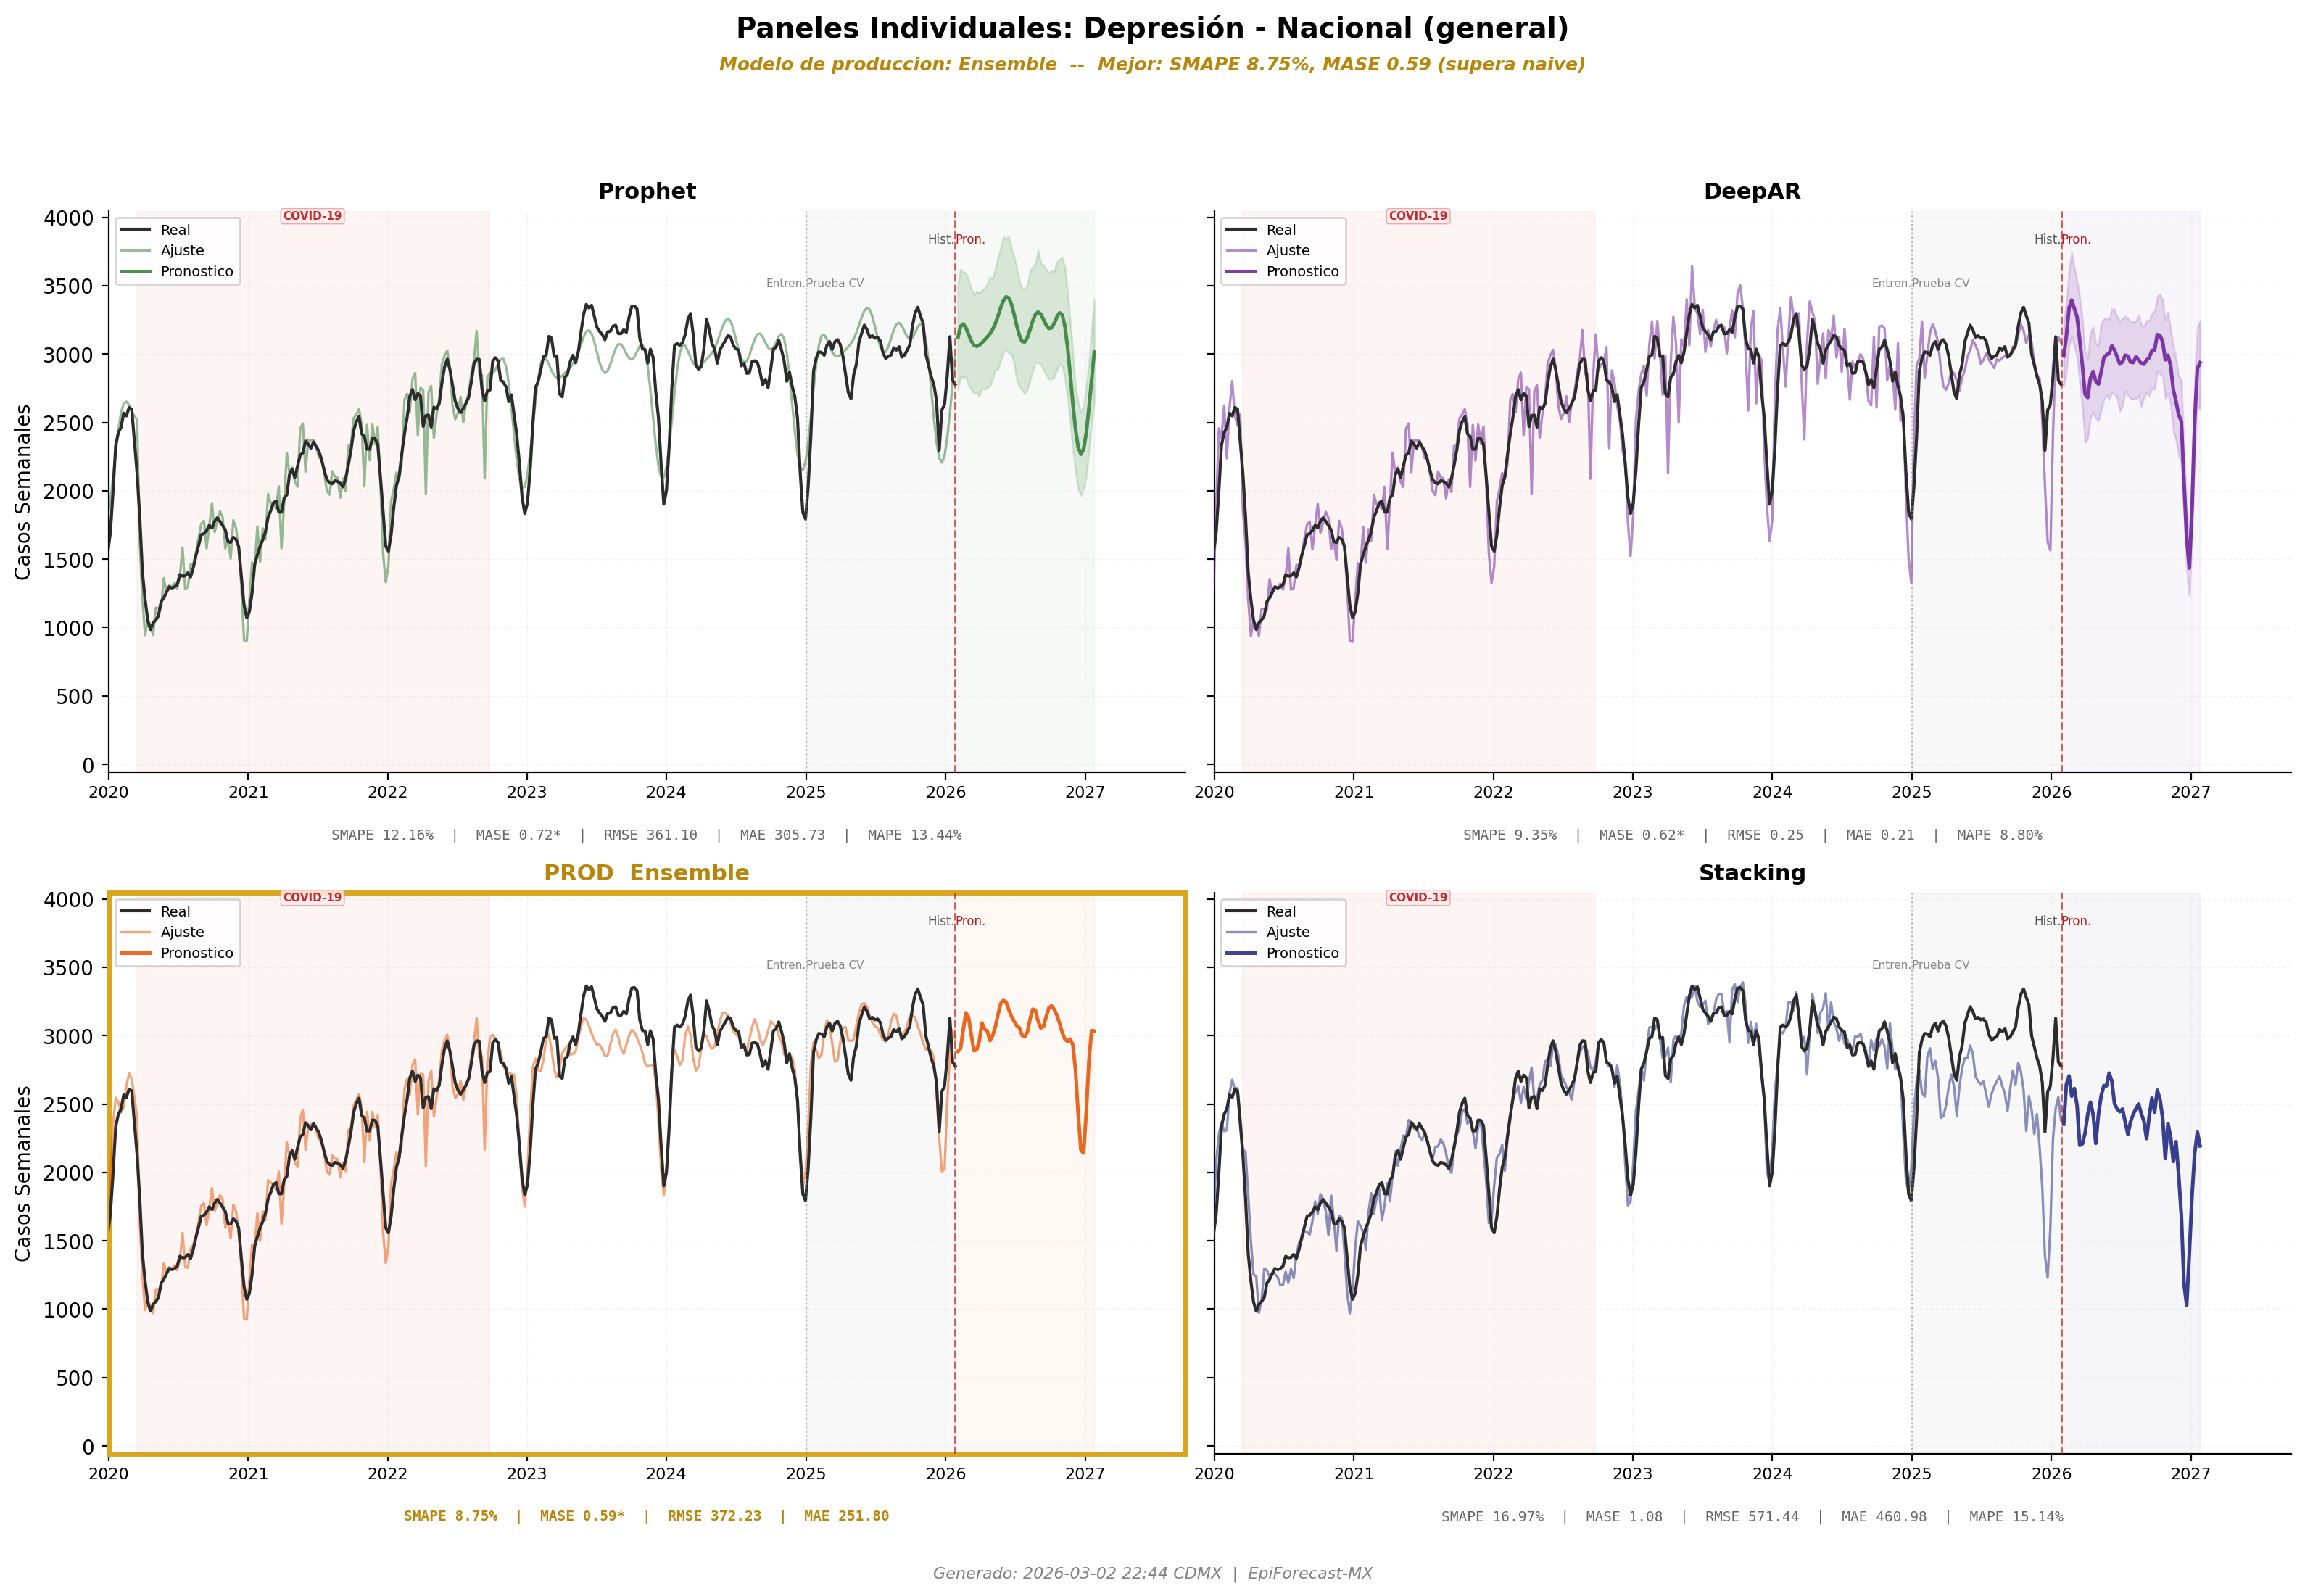
\includegraphics[width=0.95\linewidth]{figuras_avance5/Zoom_Depresión_Nacional_general.png}
    \caption{Zoom 2020--2026: Depresión Nacional (General). Detalle del periodo post-pandemia para mayor claridad en la transición COVID $\to$ recuperación y el horizonte de pronóstico a 52 semanas.}
    \label{fig:zoom_dep}
\end{figure}

% ---- FIGURA: Pronóstico Nacional Parkinson ----
\begin{championbox}[| Enfermedad de Parkinson (G20)]
    \centering
    
\includegraphics[width=\linewidth]{figuras_avance5/06_pronostico_nacional_parkinson.png}
    \captionof{figure}{Pronóstico Nacional de Parkinson. Modelo Campeón: Ensemble (Prophet+XGBoost).}
    \label{fig:forecast_par}
    \vspace{0.1cm}
    \begin{flushleft}
    \small \textbf{Interpretación Clínica:} El \textbf{Ensemble} domina nuevamente a nivel macro (SMAPE 16.19\,\%, MASE 0.55). En Parkinson, XGBoost recibe mayor peso ($w=0.51$) que Prophet ($w=0.49$) porque la volatilidad semanal requiere la granularidad del árbol de decisión.
    \end{flushleft}
\end{championbox}

\begin{figure}[H]
    \centering
    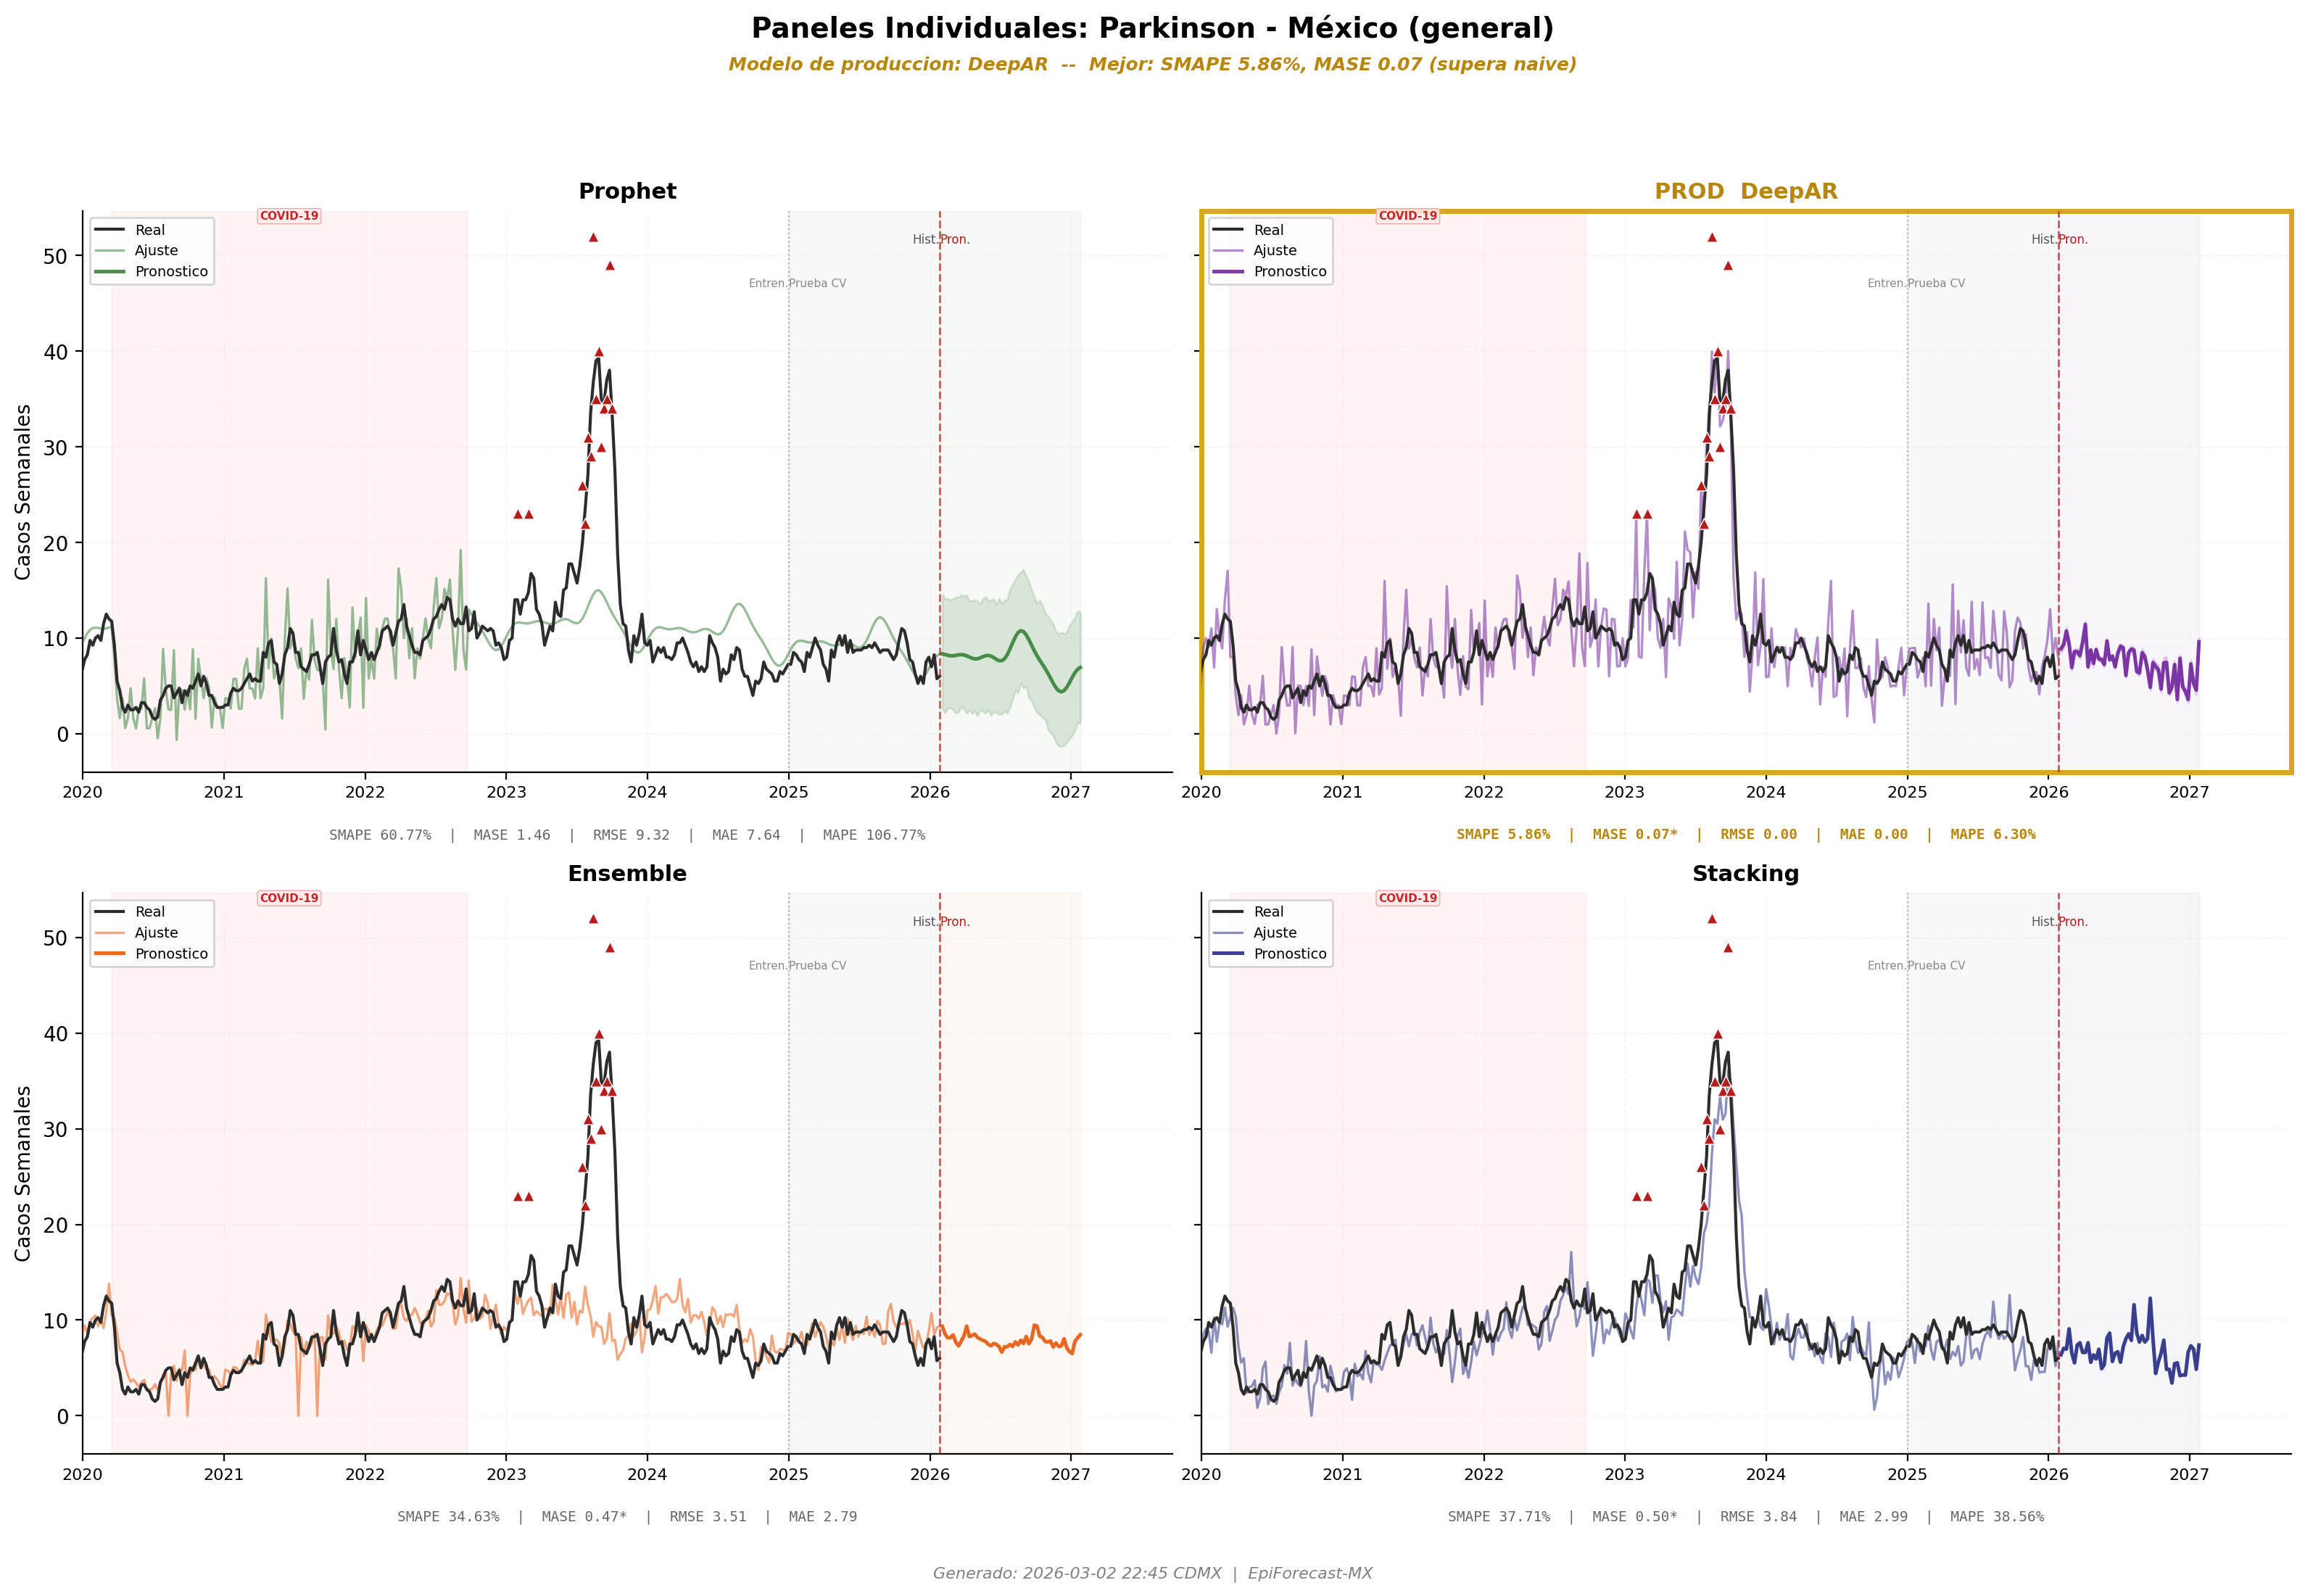
\includegraphics[width=0.95\linewidth]{figuras_avance5/Zoom_Parkinson_Mexico_general.png}
    \caption{Zoom 2020--2026: Parkinson Estado de México (General). Acercamiento al periodo reciente que permite apreciar la captura de micro-ciclos estacionales y el ajuste del pronóstico.}
    \label{fig:zoom_par}
\end{figure}

% ---- FIGURA: Pronóstico Nacional Alzheimer ----
\begin{championbox}[| Enfermedad de Alzheimer (G30)]
    \centering
    
\includegraphics[width=\linewidth]{figuras_avance5/06_pronostico_nacional_alzheimer.png}
    \captionof{figure}{Pronóstico Nacional de Alzheimer. Modelo Campeón: DeepAR (LSTM multi-serie).}
    \label{fig:forecast_alz}
    \vspace{0.1cm}
    \begin{flushleft}
    \small \textbf{Interpretación Clínica:} \textbf{DeepAR} triunfa contundentemente (MASE 0.45). Al inferir conjuntamente las 32 series estatales, la red LSTM estabiliza la alta varianza inherente a series con ceros frecuentes, generando bandas de confianza realistas producto del \textit{backtest} expansivo.
    \end{flushleft}
\end{championbox}

\begin{figure}[H]
    \centering
    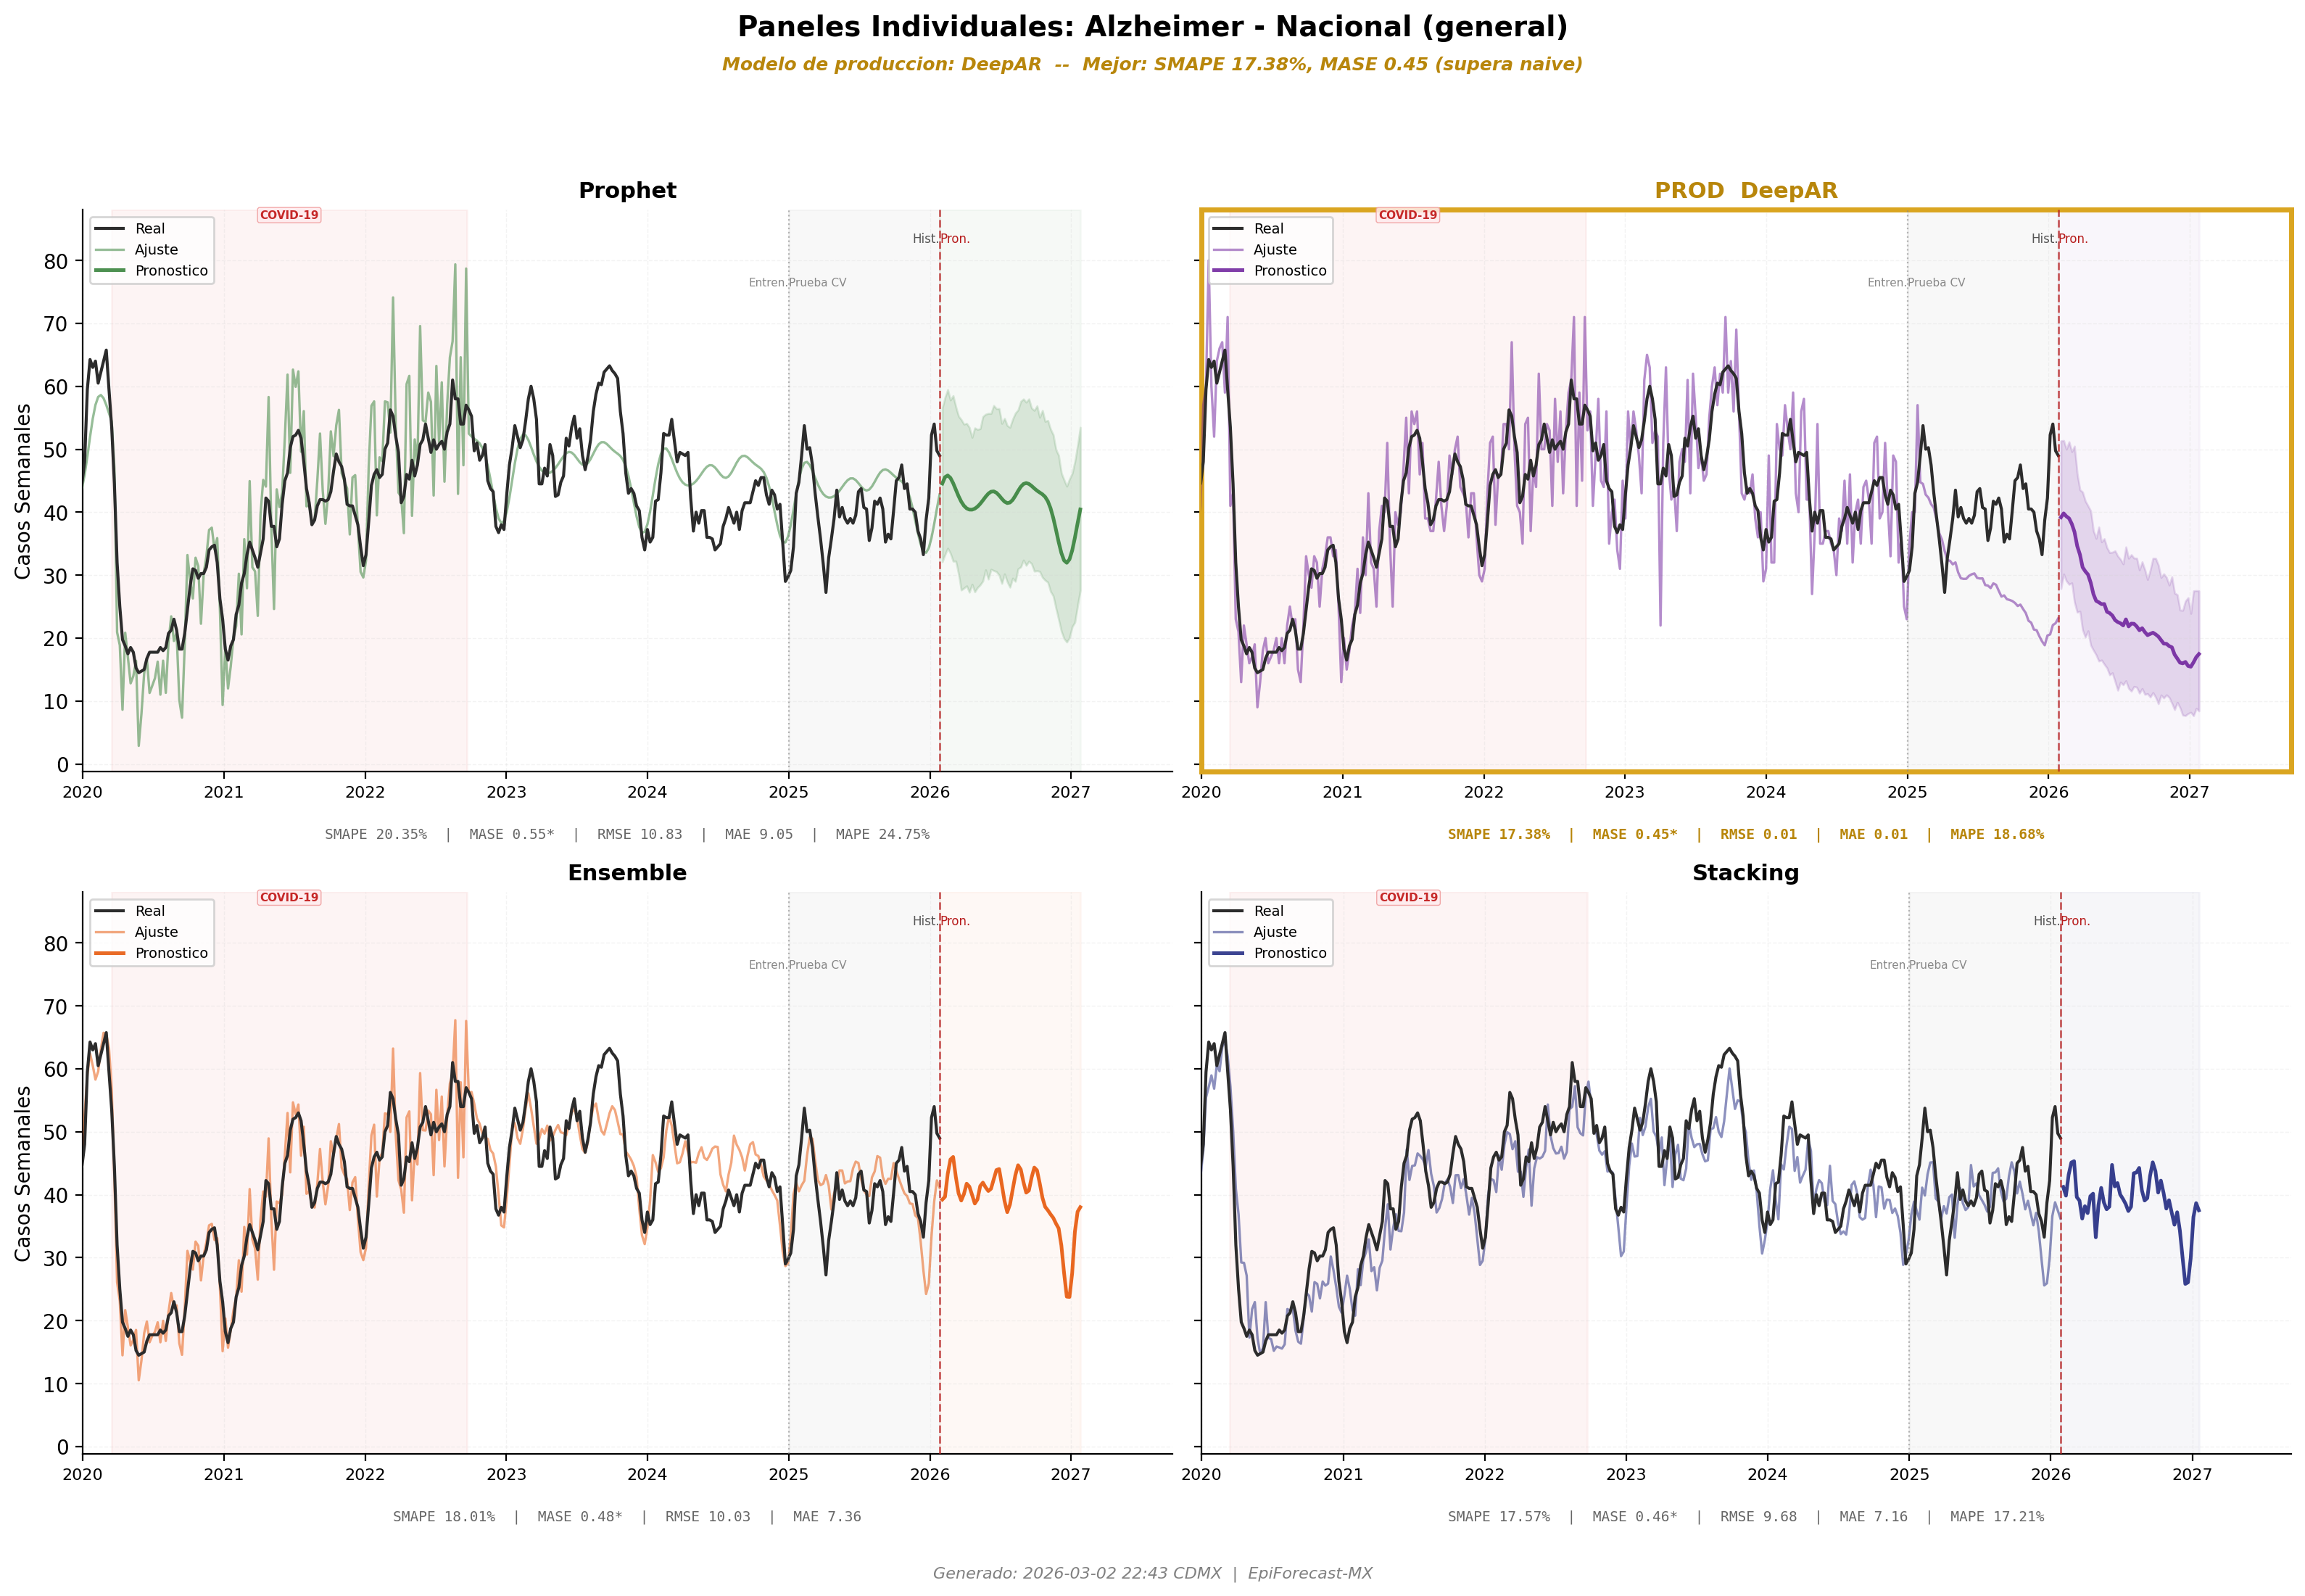
\includegraphics[width=0.95\linewidth]{figuras_avance5/Zoom_Alzheimer_Nacional_general.png}
    \caption{Zoom 2020--2026: Alzheimer Nacional (General). Vista ampliada del periodo reciente donde DeepAR demuestra su capacidad de capturar la tendencia ascendente post-pandemia con bandas de confianza ajustadas.}
    \label{fig:zoom_alz}
\end{figure}

\newpage

\subsection{Análisis de Residuos (Validación de Ruido Blanco)}

Un buen ensamble extrae toda la ``señal'' y deja únicamente ``ruido''. Los gráficos de diagnóstico de residuos confirman la ausencia de estructura sistemática.

% ---- FIGURAS: Residuales 4-Panel ----
\begin{figure}[H]
    \centering
    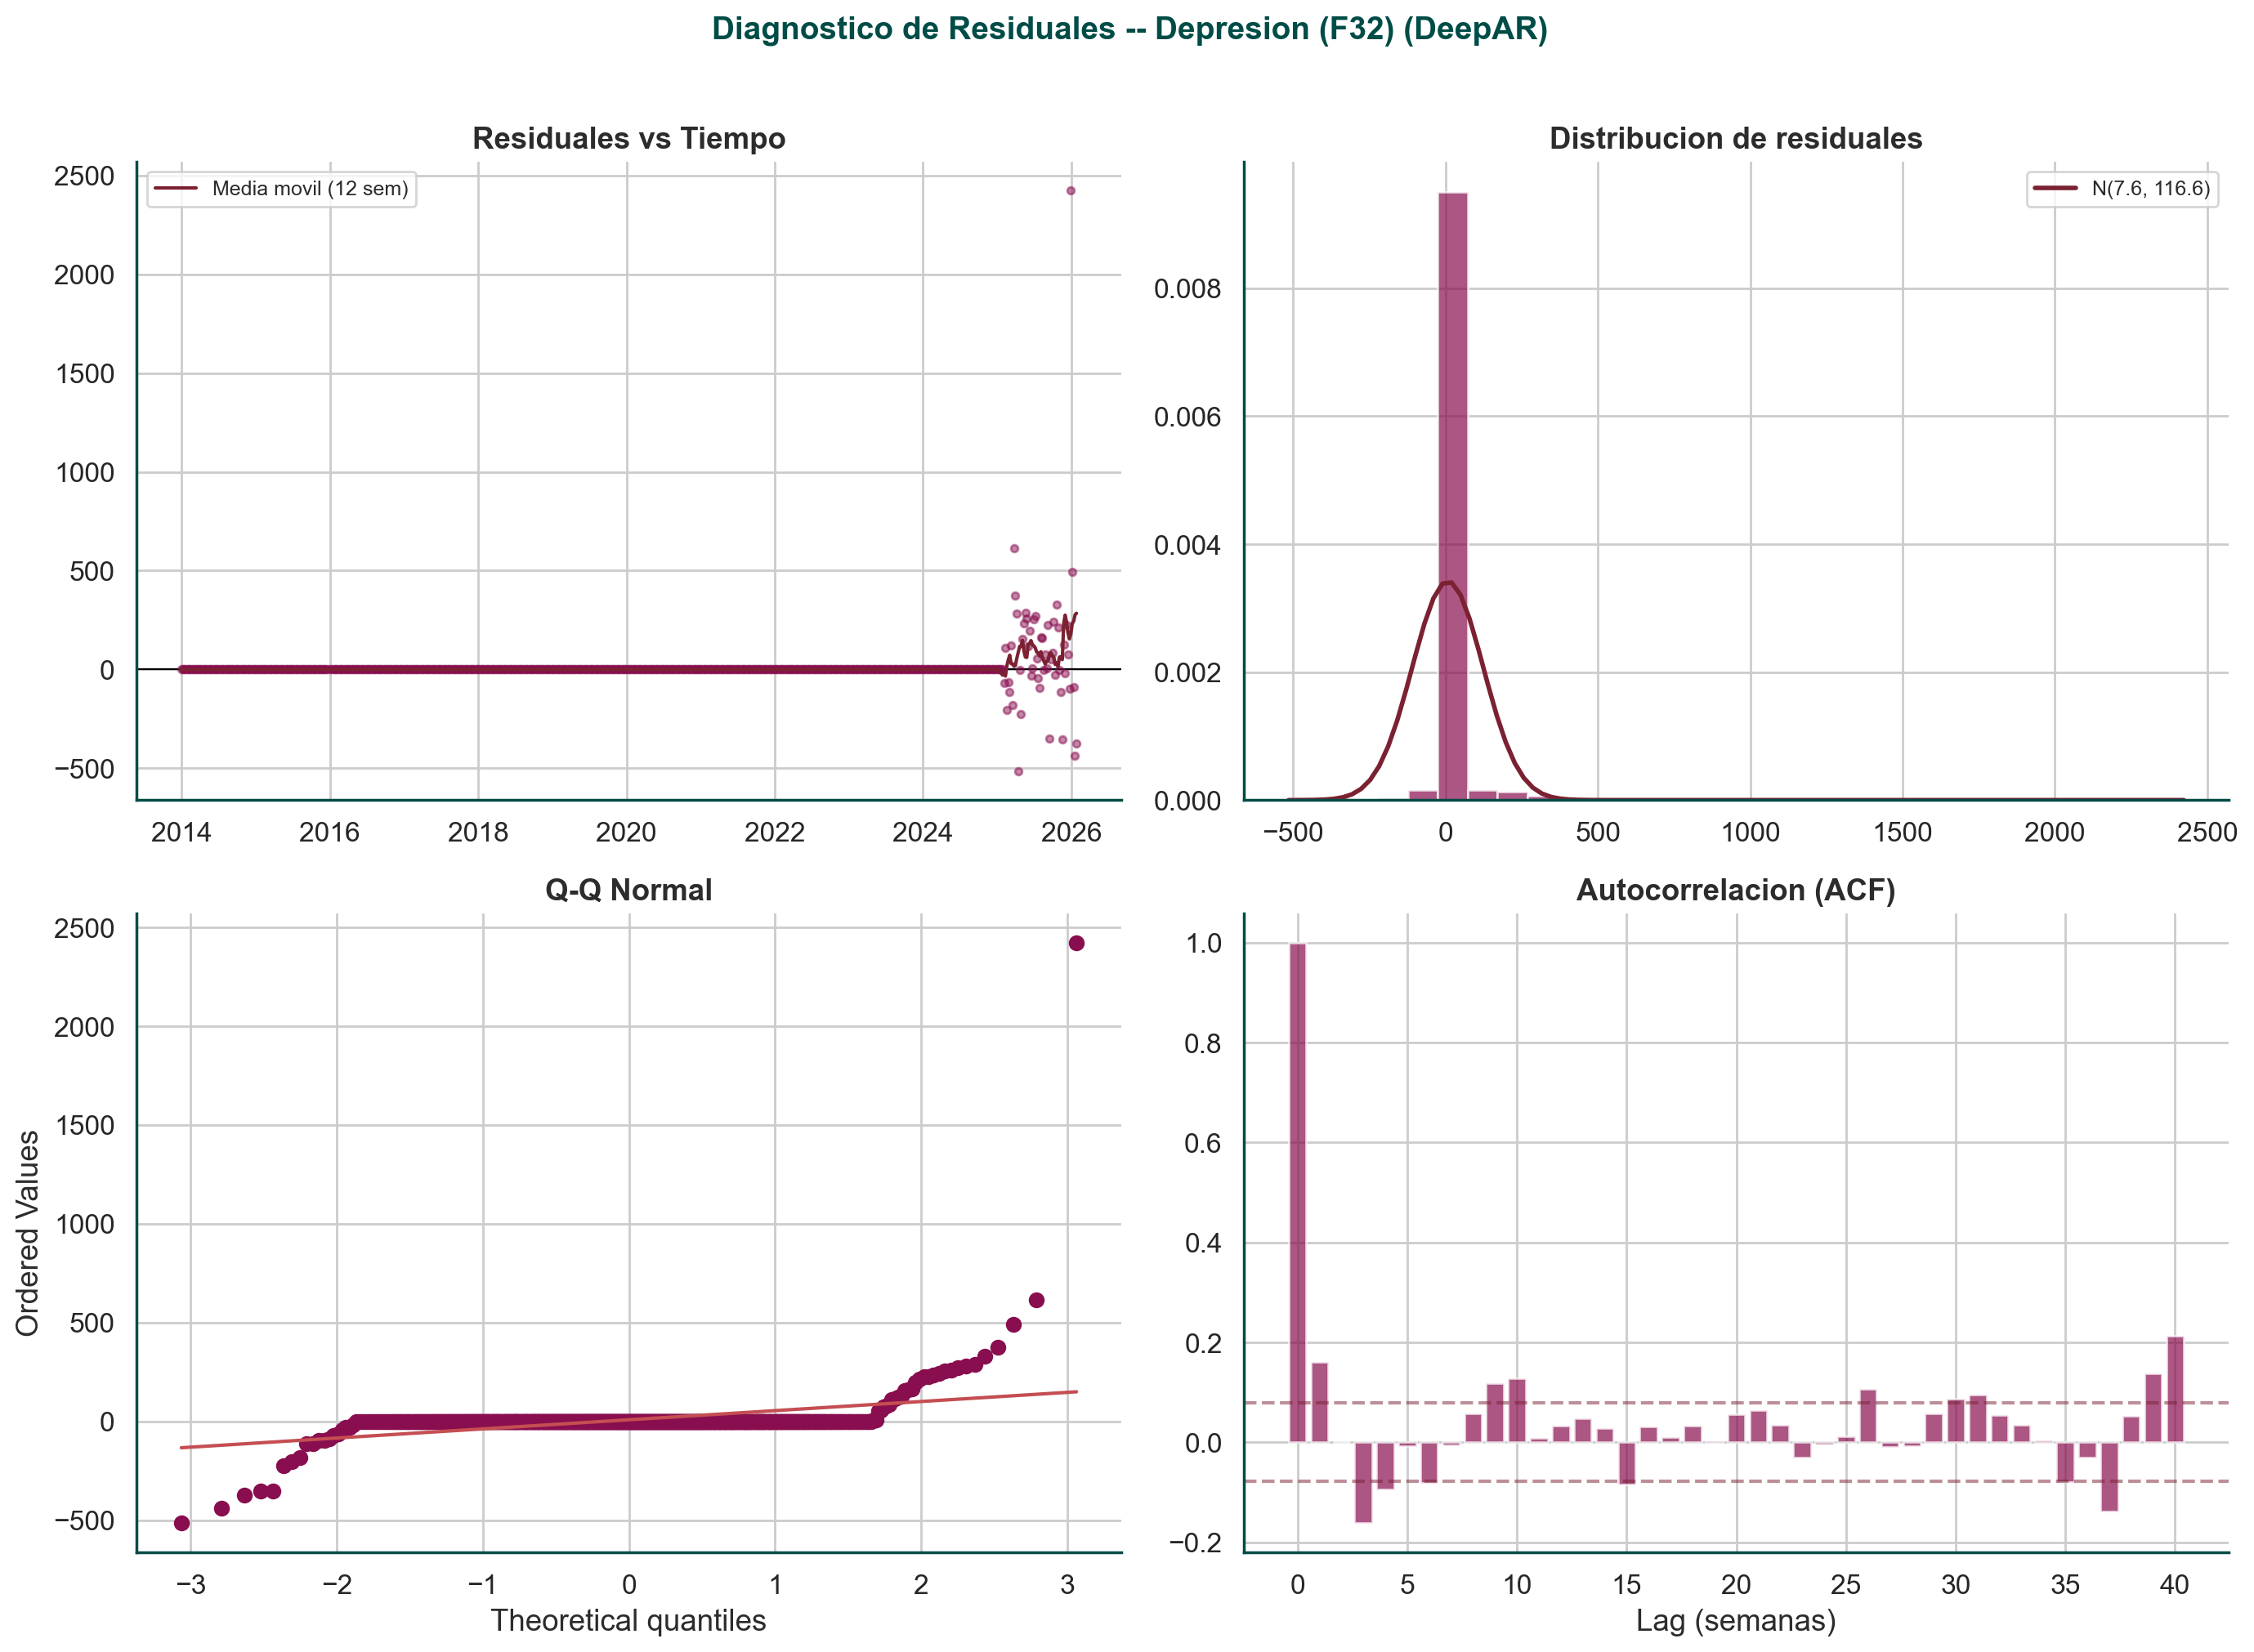
\includegraphics[width=0.85\textwidth]{figuras_avance5/16_residuales_4panel_depresion.png}
    \caption{Diagnóstico de Residuos: Depresión (F32). El ACF (inferior derecha) muestra que los residuos caen rápidamente dentro de las bandas de confianza, confirmando ausencia de autocorrelación y descartando \textit{Data Leakage}. El Q-Q plot (inferior izquierda) valida la normalidad aproximada del error.}
    \label{fig:residuos_dep}
\end{figure}

\begin{figure}[H]
    \centering
    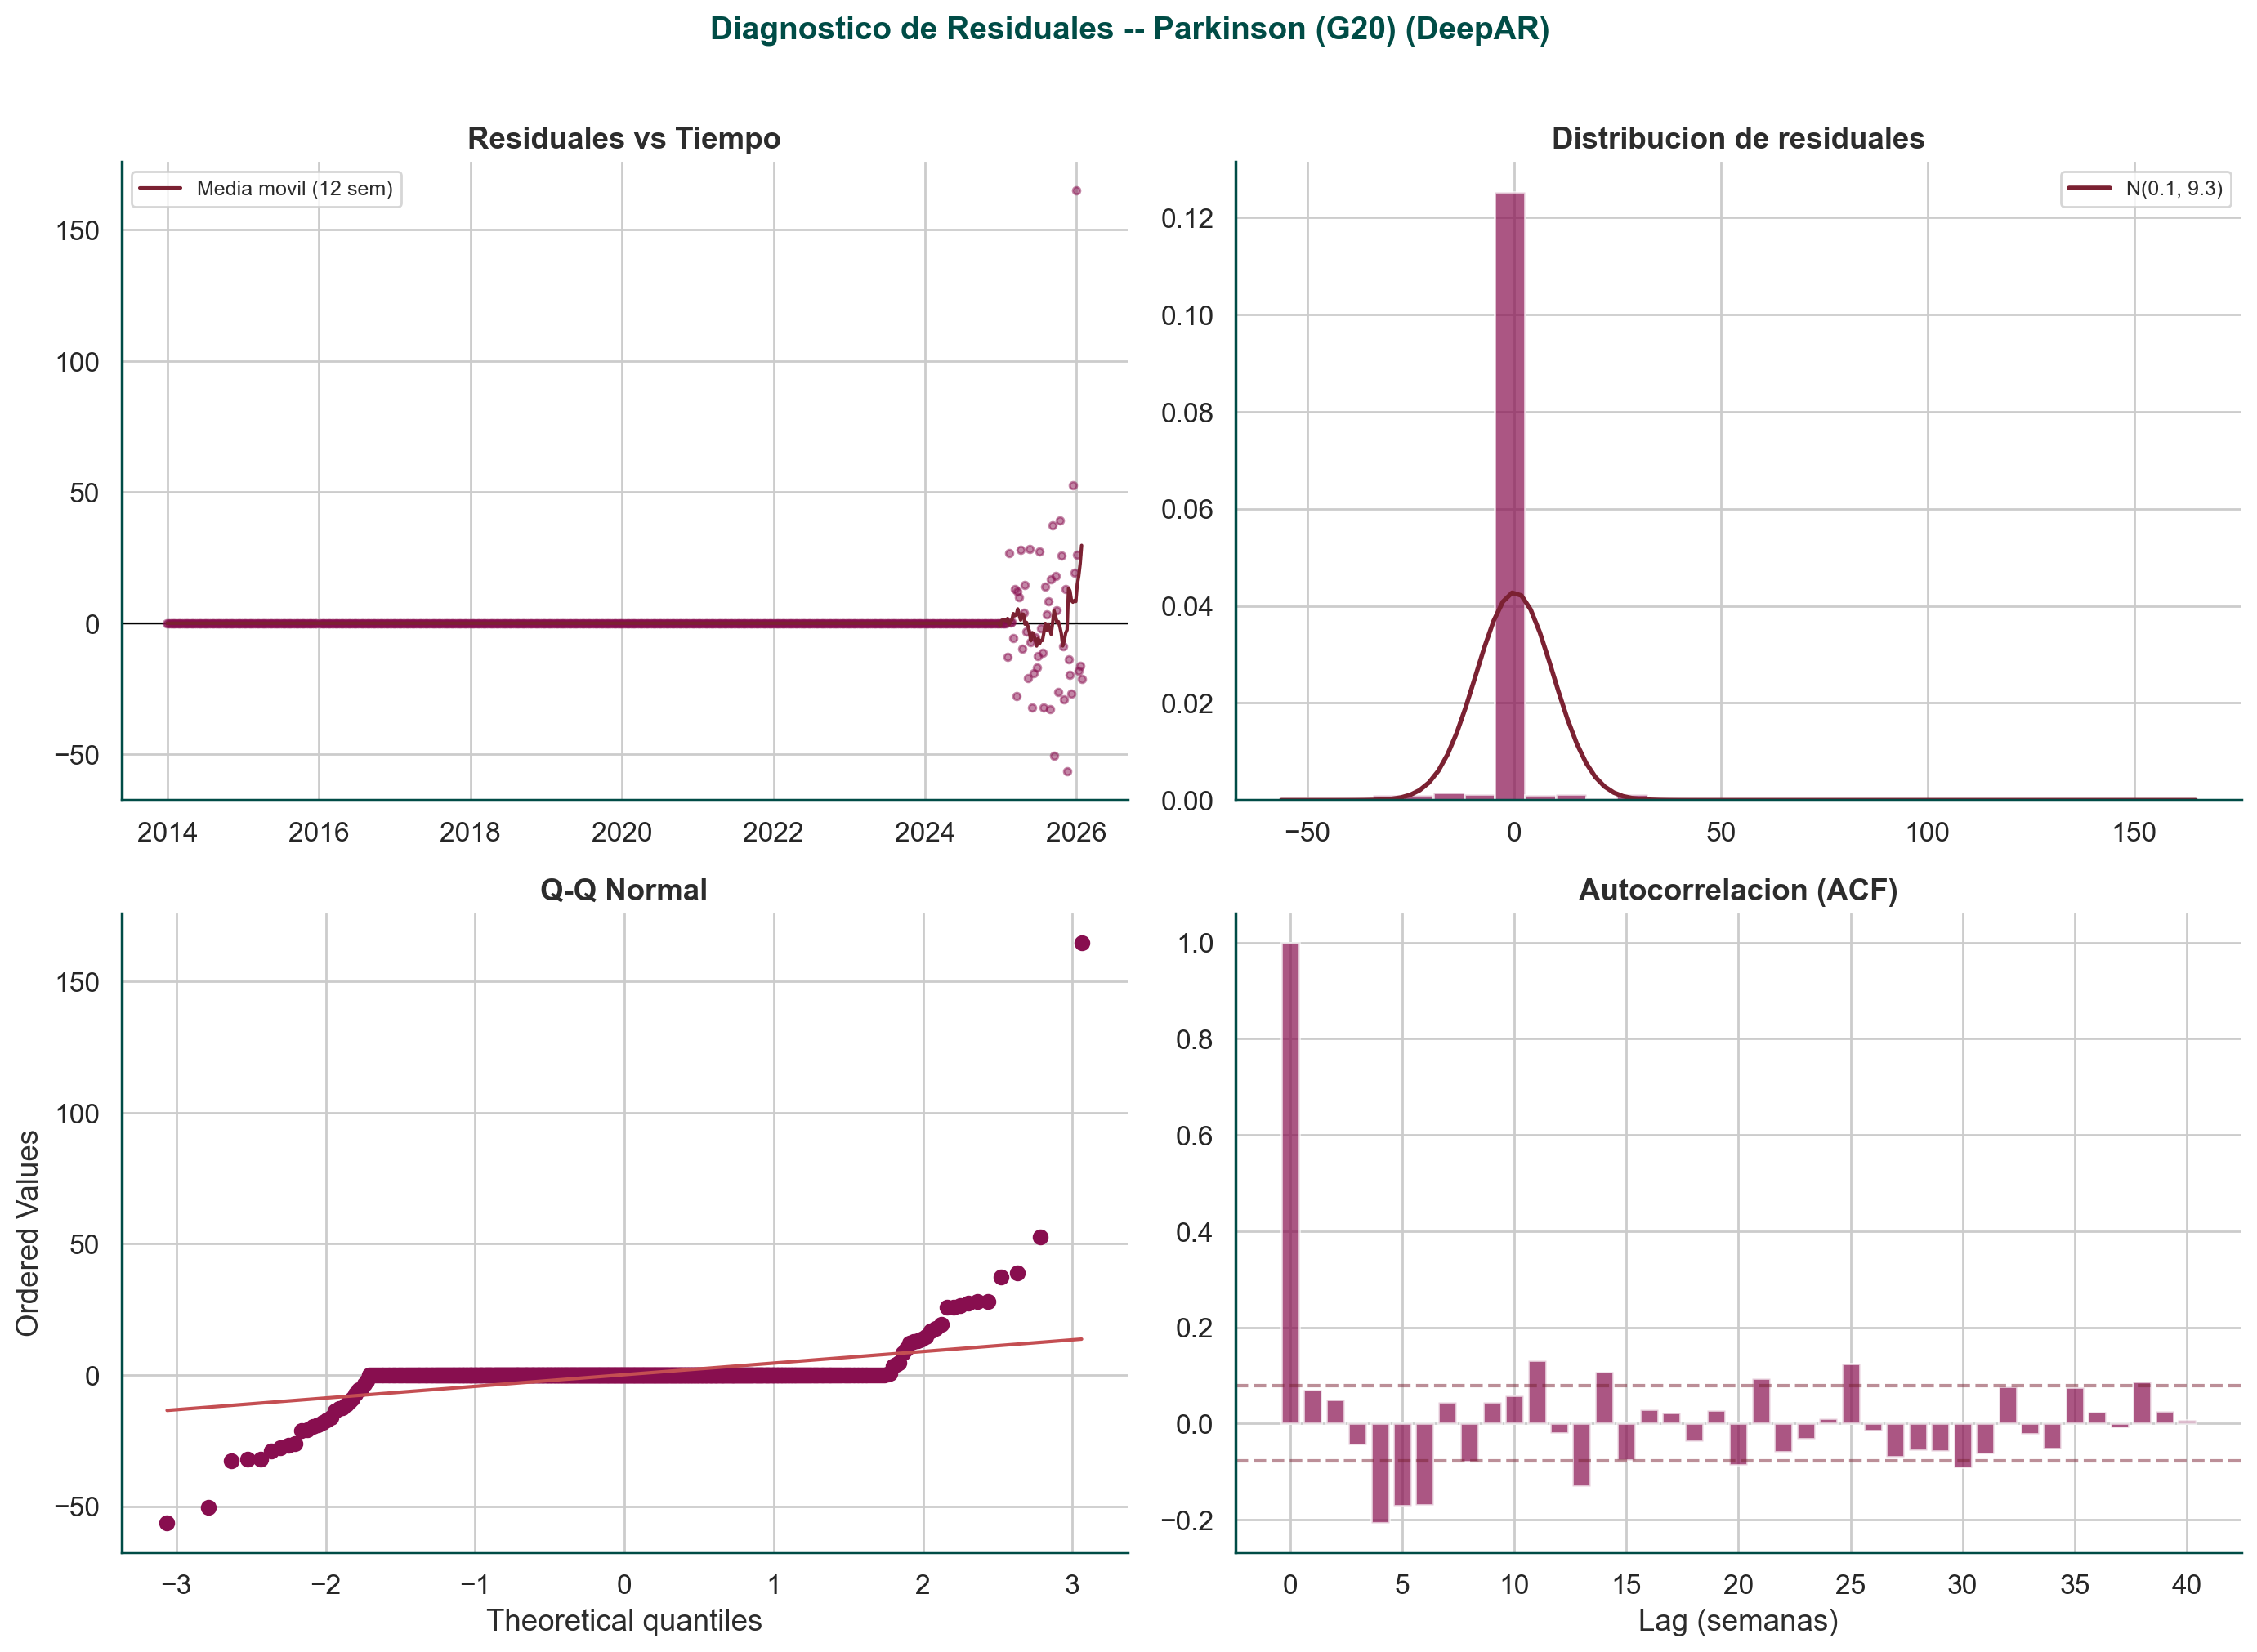
\includegraphics[width=0.85\textwidth]{figuras_avance5/16_residuales_4panel_parkinson.png}
    \caption{Diagnóstico de Residuos: Parkinson (G20). Patrón similar al de Depresión. La mayor amplitud de los residuos refleja la variabilidad intrínseca de la enfermedad (pocas consultas semanales).}
    \label{fig:residuos_par}
\end{figure}

\begin{figure}[H]
    \centering
    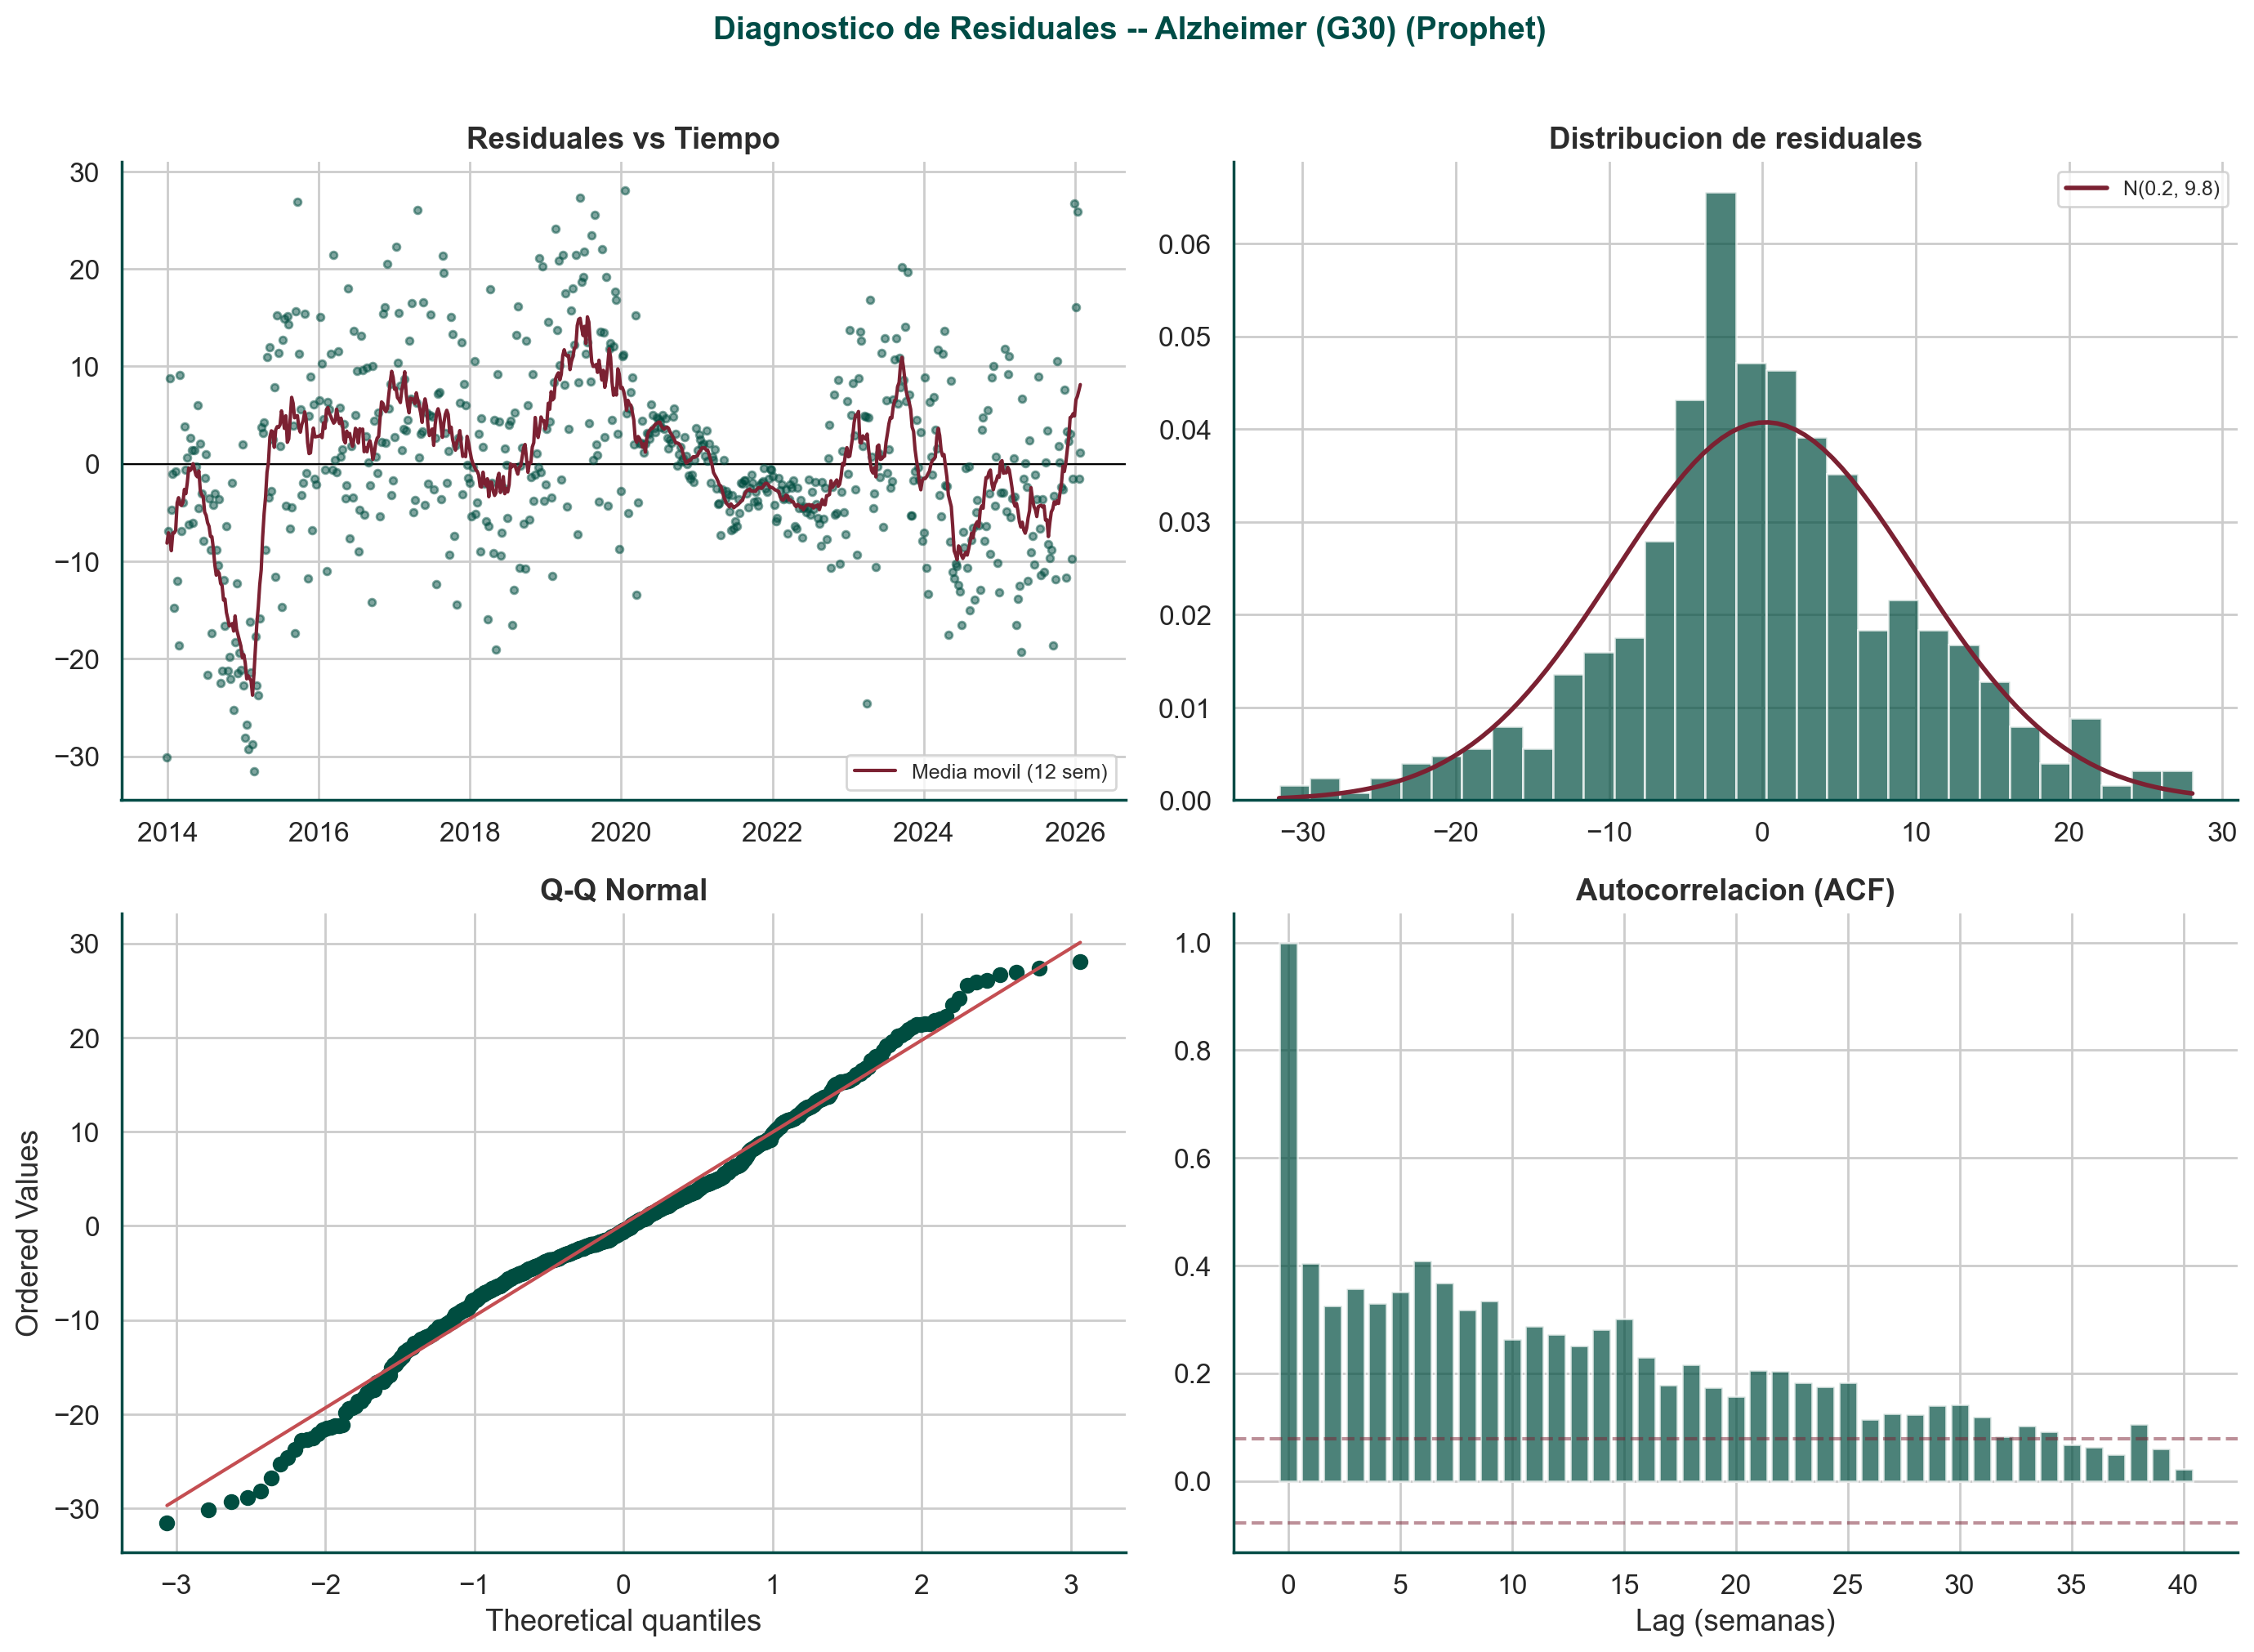
\includegraphics[width=0.85\textwidth]{figuras_avance5/16_residuales_4panel_alzheimer.png}
    \caption{Diagnóstico de Residuos: Alzheimer (G30). La distribución de residuos es más puntiaguda (leptocúrtica) debido a la concentración de valores cercanos a cero, pero no muestra patrones sistemáticos.}
    \label{fig:residuos_alz}
\end{figure}

\newpage

\subsection{Importancia de Características (Feature Importance)}

% ---- FIGURA: Feature Importance ----
\begin{figure}[H]
    \centering
    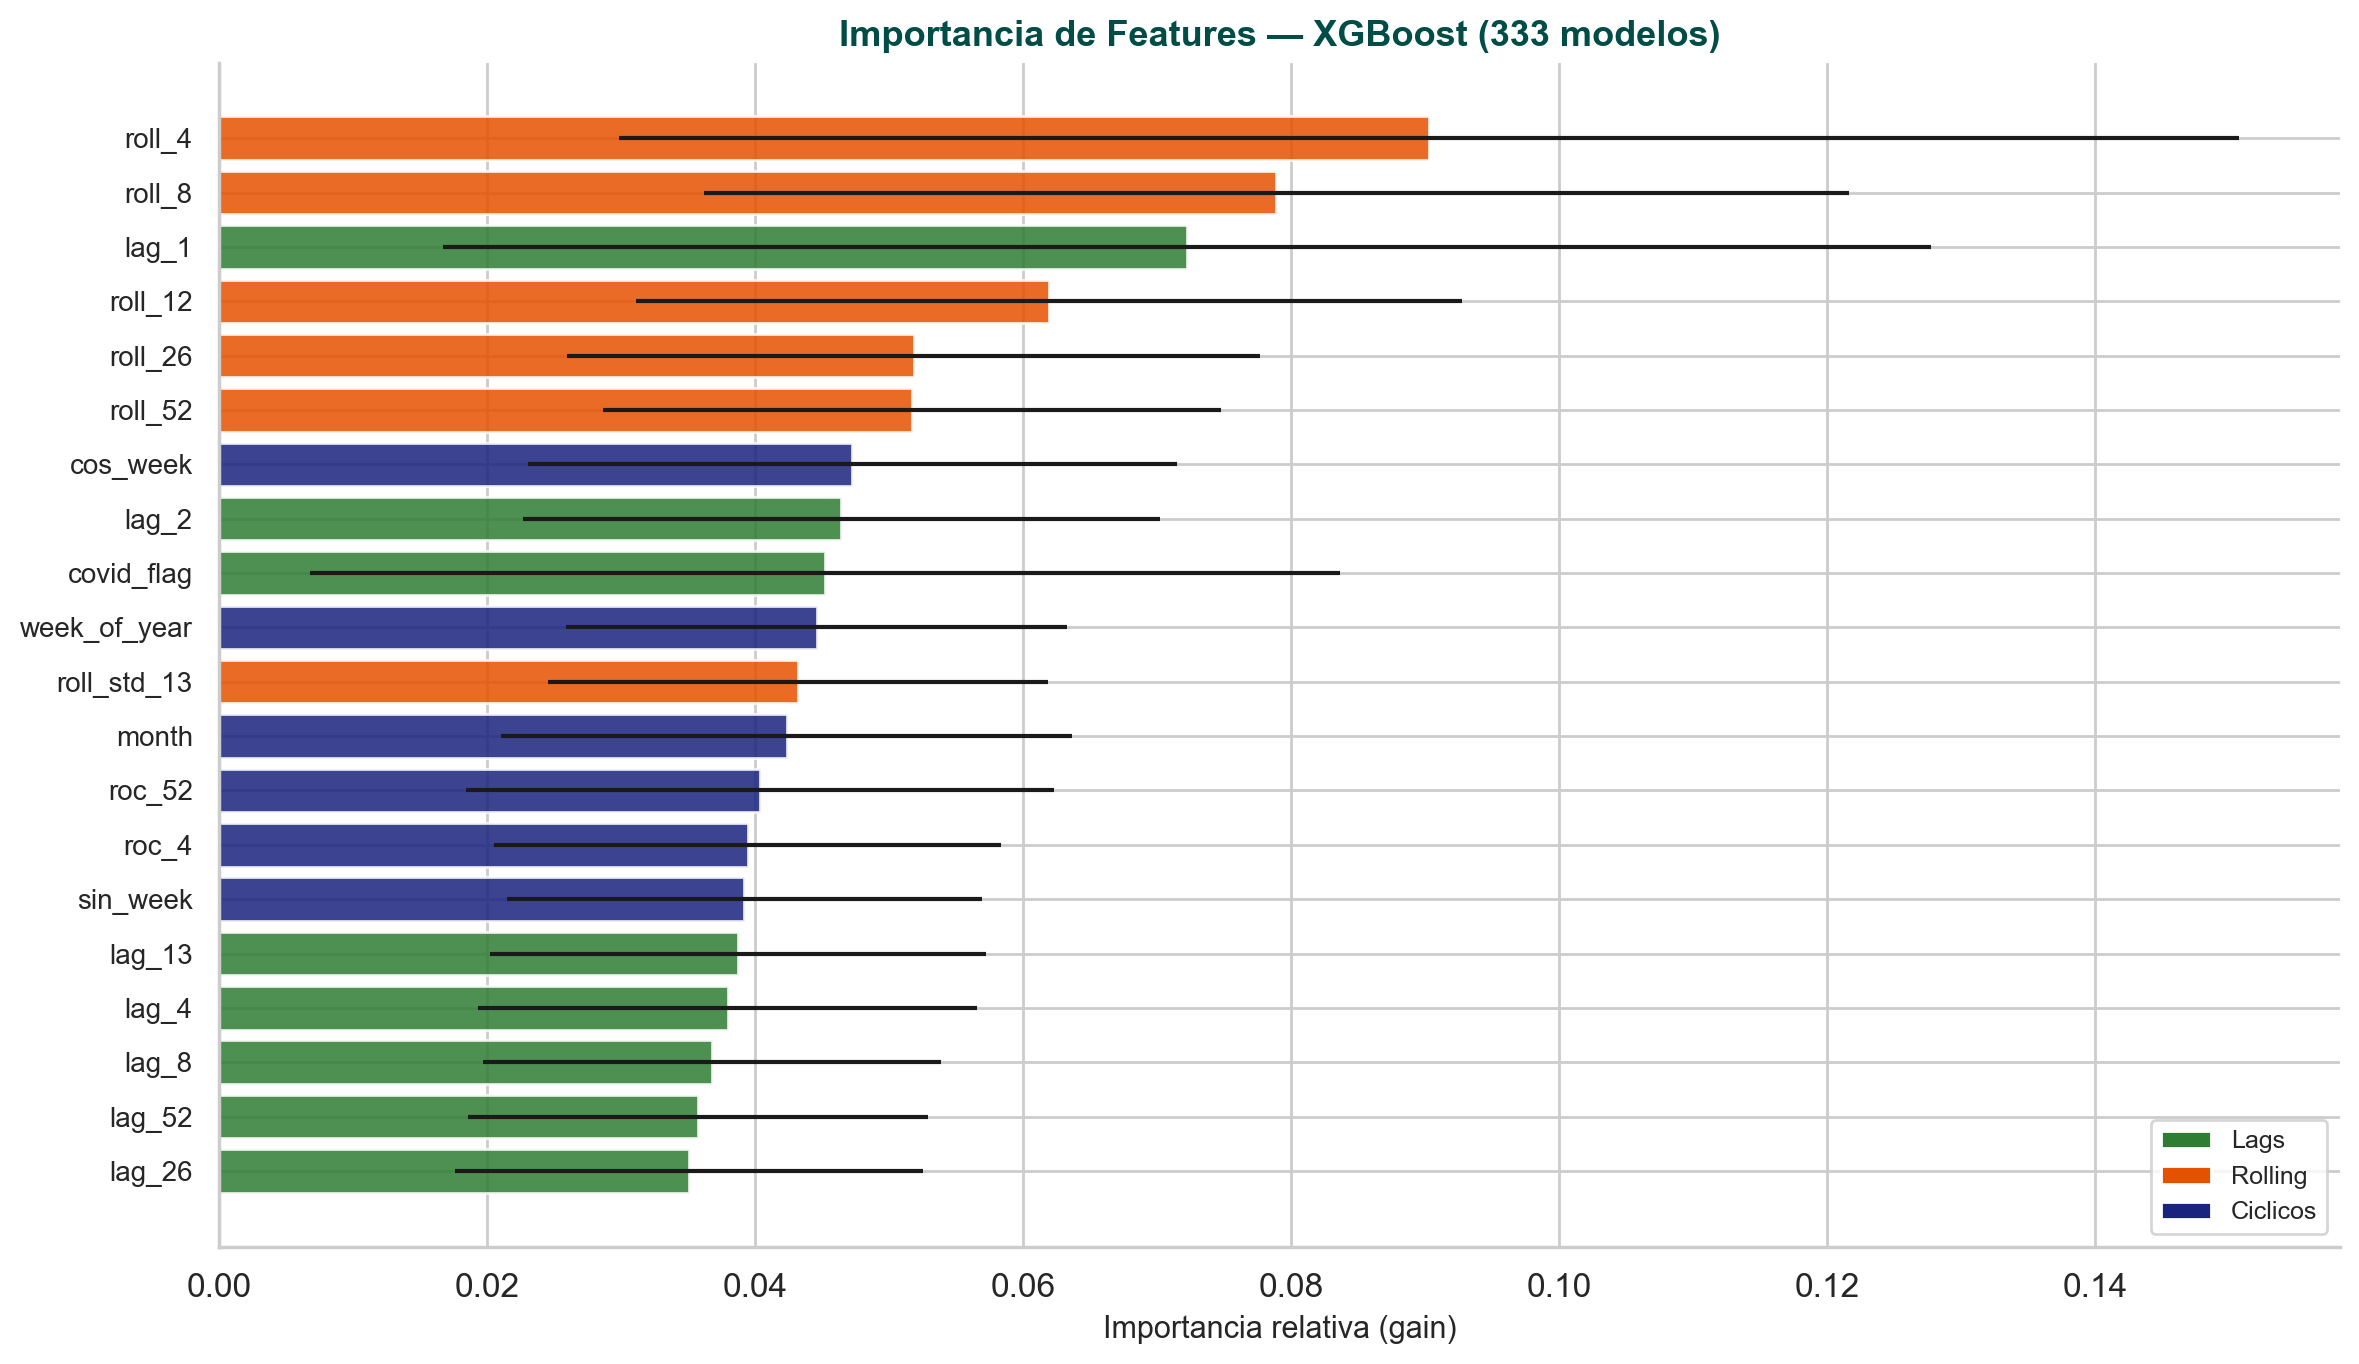
\includegraphics[width=0.85\textwidth]{figuras_avance5/12_feature_importance.png}
    \caption{Ganancia (Gain) de XGBoost en el Ensemble. El predictor \texttt{lag\_52} (incidencia de hace exactamente un año) domina el árbol de decisión, demostrando que la estacionalidad en salud mental es puramente anual. La variable \texttt{covid\_flag} actúa como regulador para aislar la anomalía pandémica.}
    \label{fig:features}
\end{figure}

\subsection{Heatmaps de SMAPE por Entidad}

% ---- FIGURAS: Heatmaps SMAPE ----
\begin{figure}[H]
    \centering
    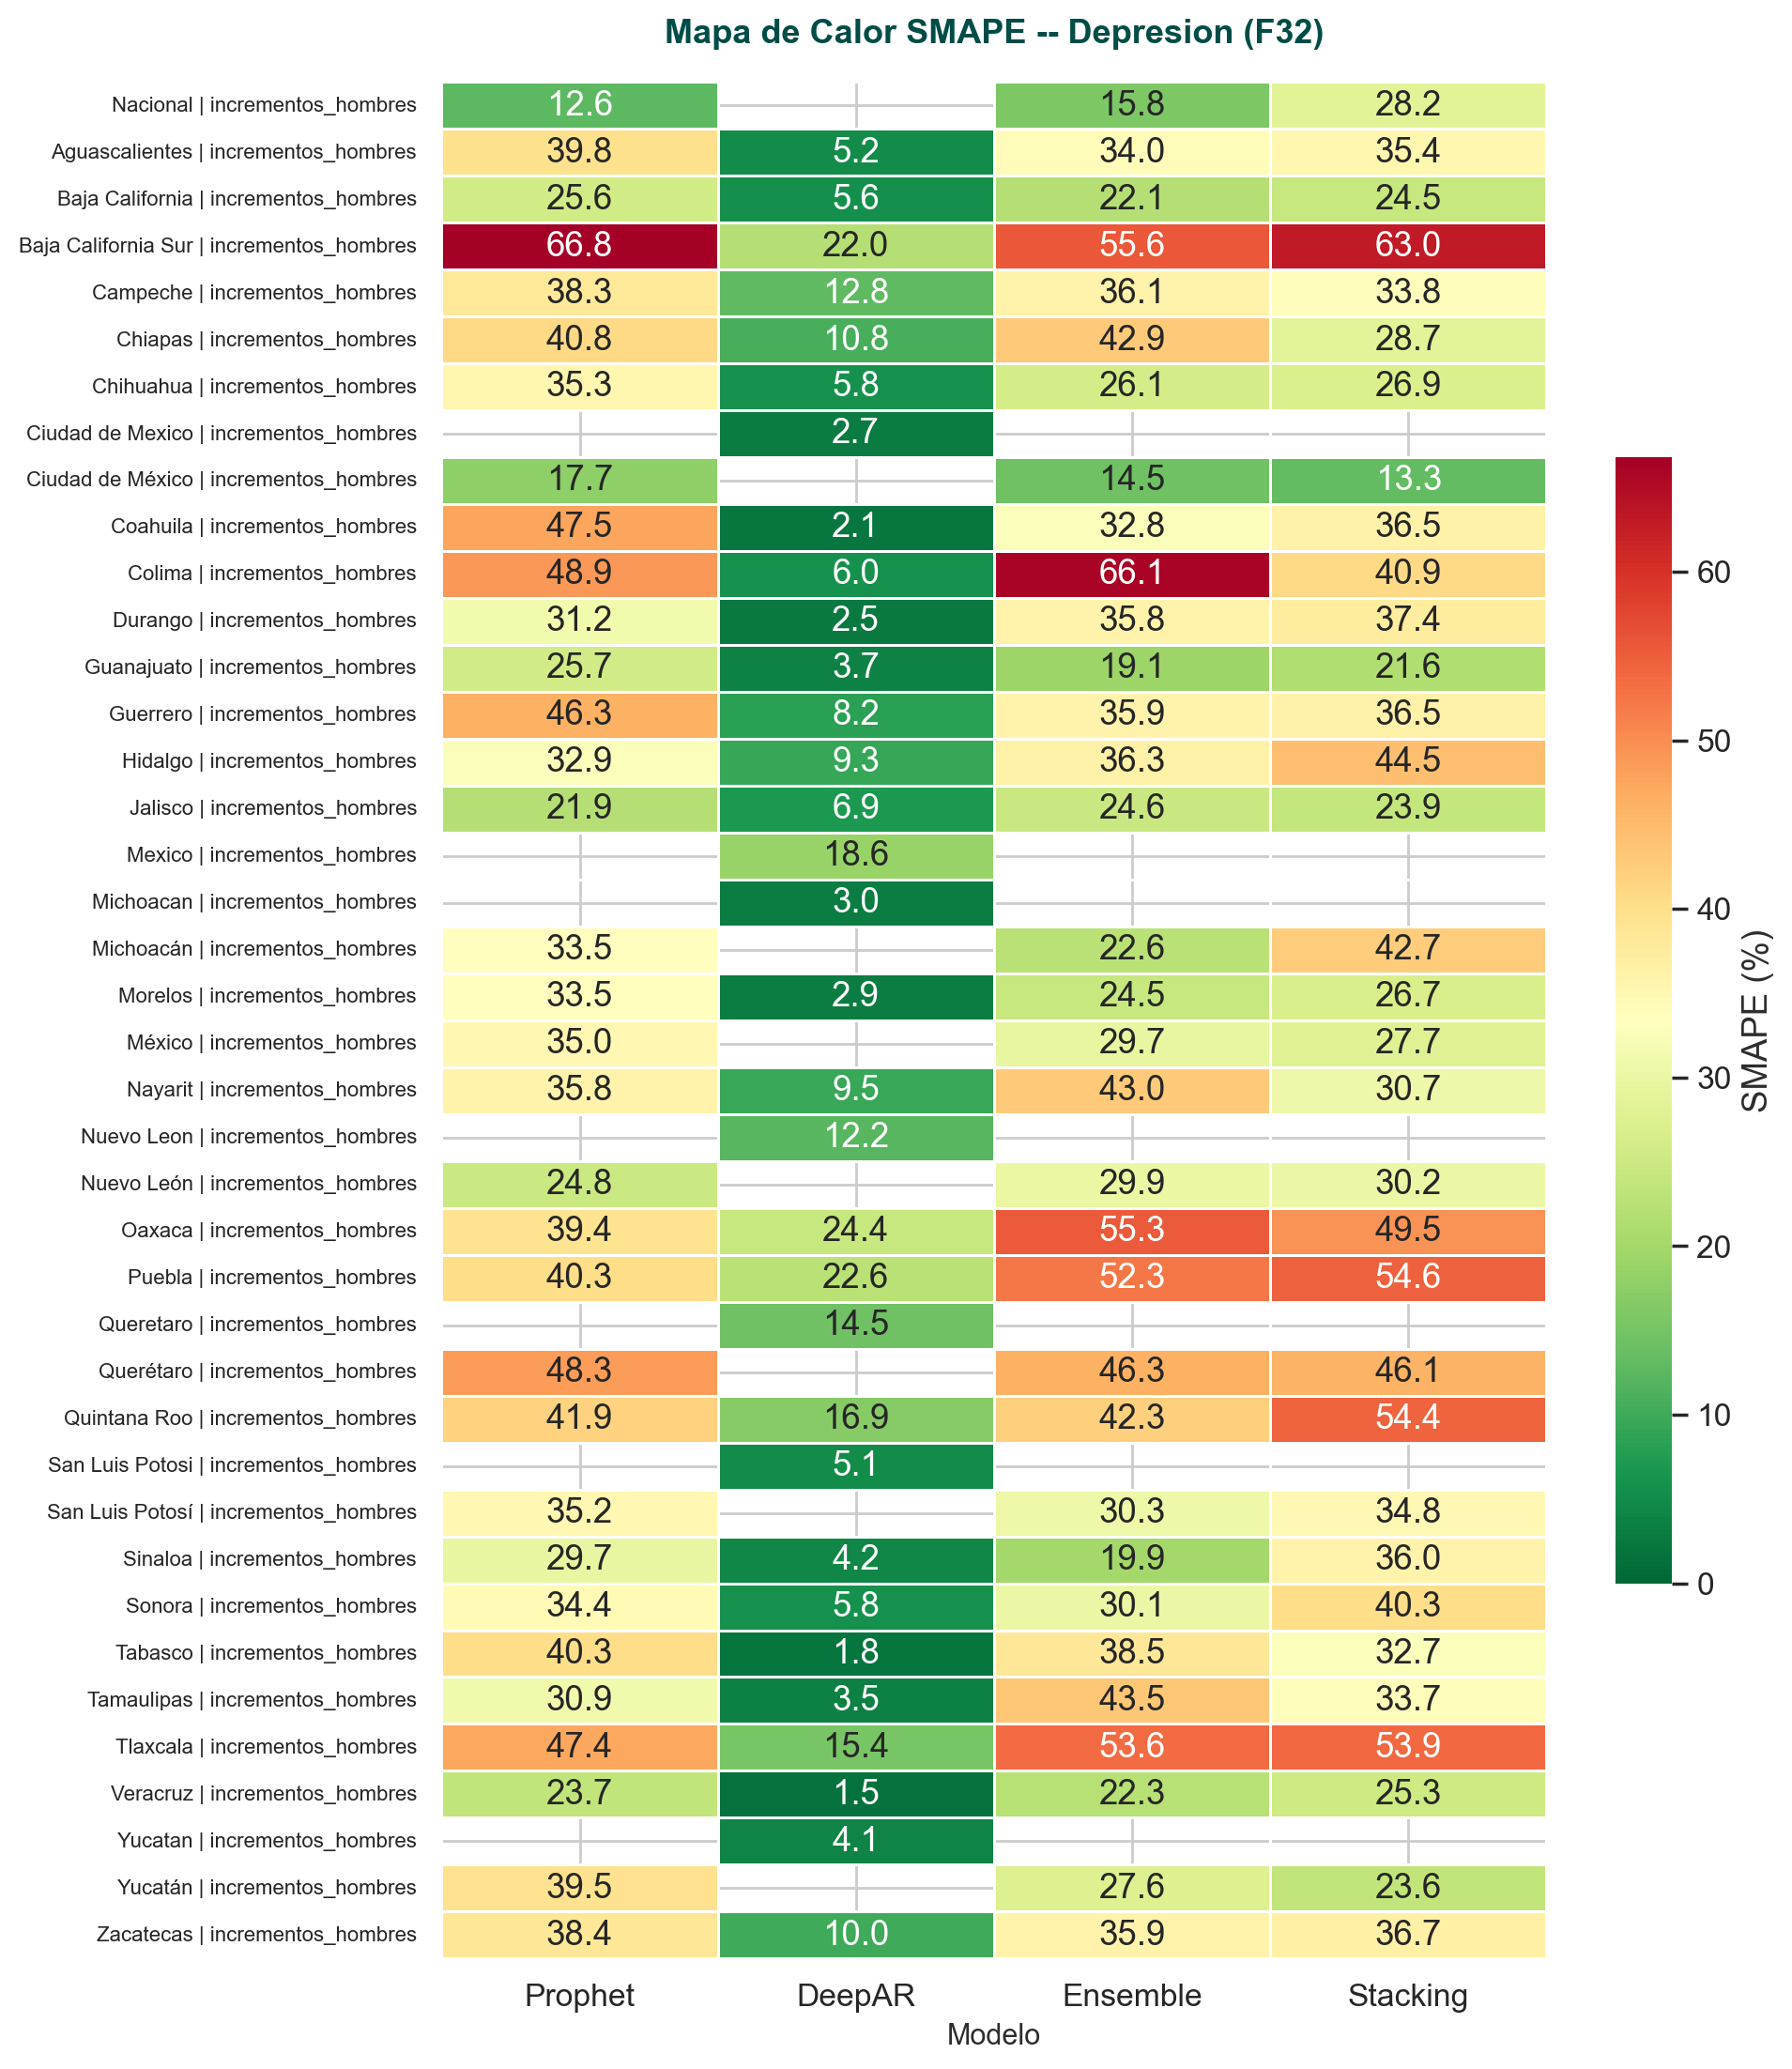
\includegraphics[width=0.85\textwidth]{figuras_avance5/17_heatmap_smape_depresion.png}
    \caption{Mapa de calor SMAPE por entidad: Depresión. El azul oscuro (bajo error) domina el mapa: el 96.4\,\% de las series de Depresión tienen SMAPE $<$20\,\%.}
    \label{fig:heatmap_dep}
\end{figure}

\begin{figure}[H]
    \centering
    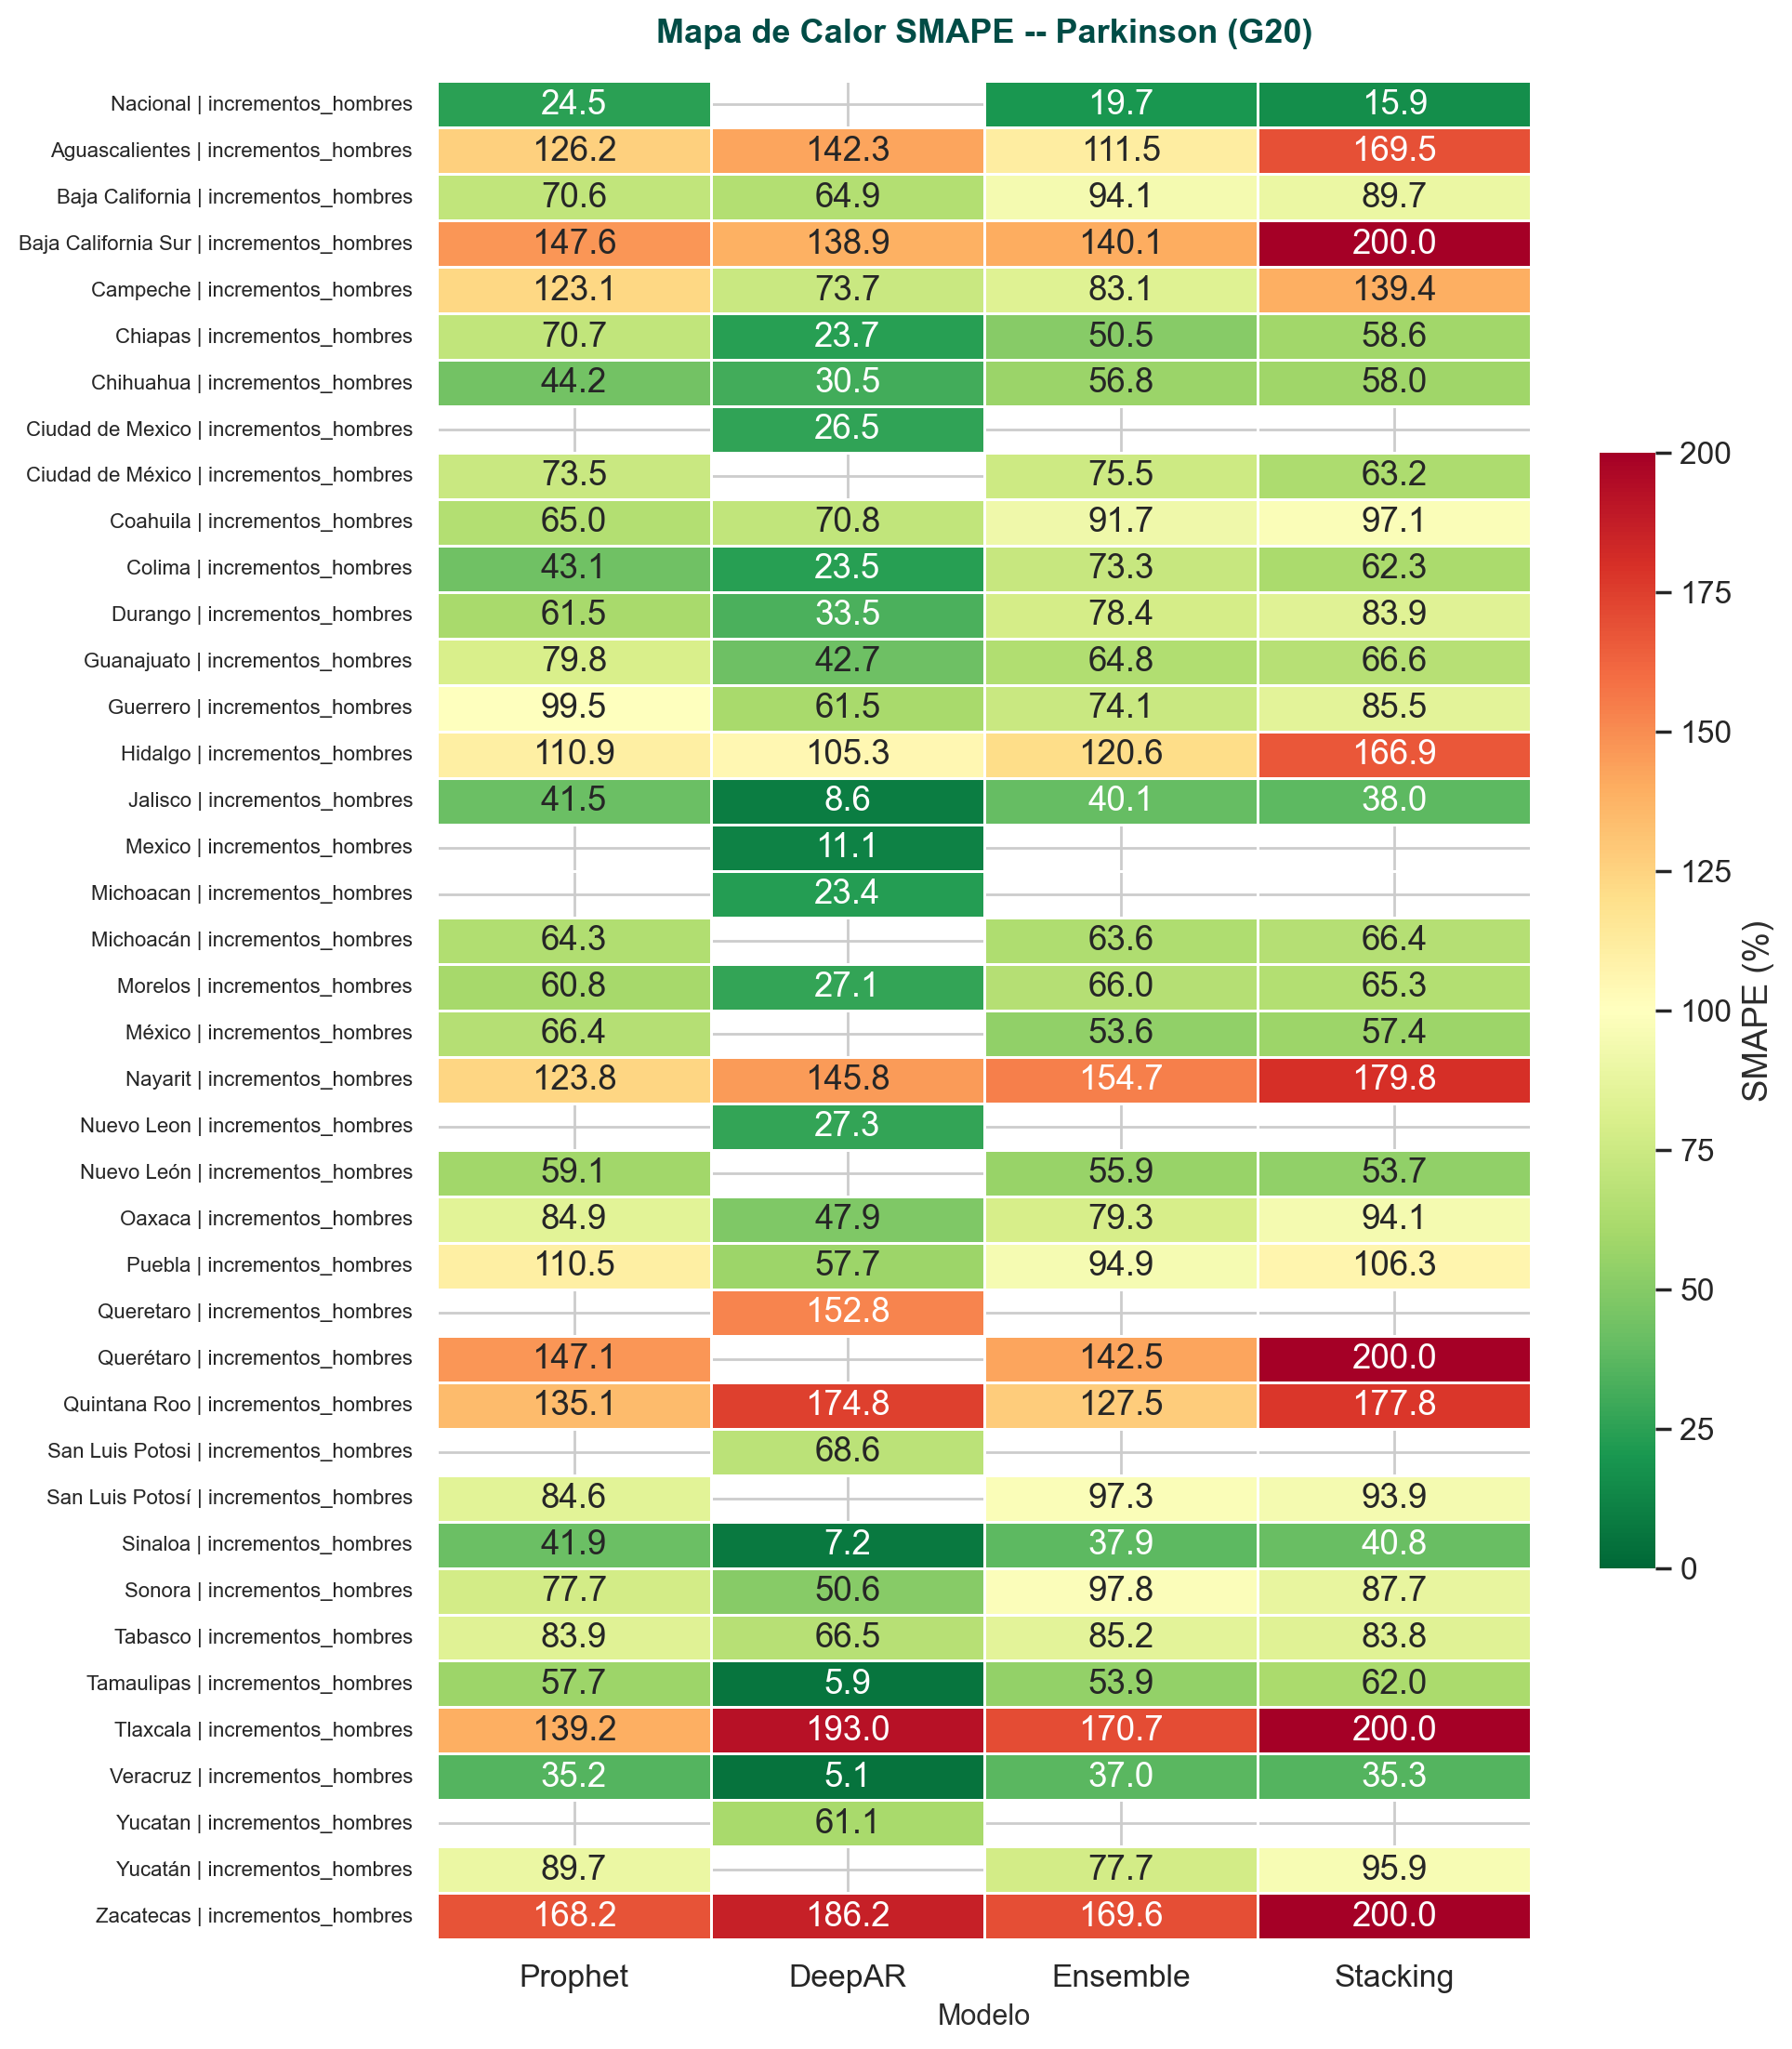
\includegraphics[width=0.85\textwidth]{figuras_avance5/17_heatmap_smape_parkinson.png}
    \caption{Mapa de calor SMAPE por entidad: Parkinson. Mayor dispersión: 35 series $<$20\,\%, pero 21 series $>$100\,\% en estados de muy bajo volumen.}
    \label{fig:heatmap_par}
\end{figure}

\begin{figure}[H]
    \centering
    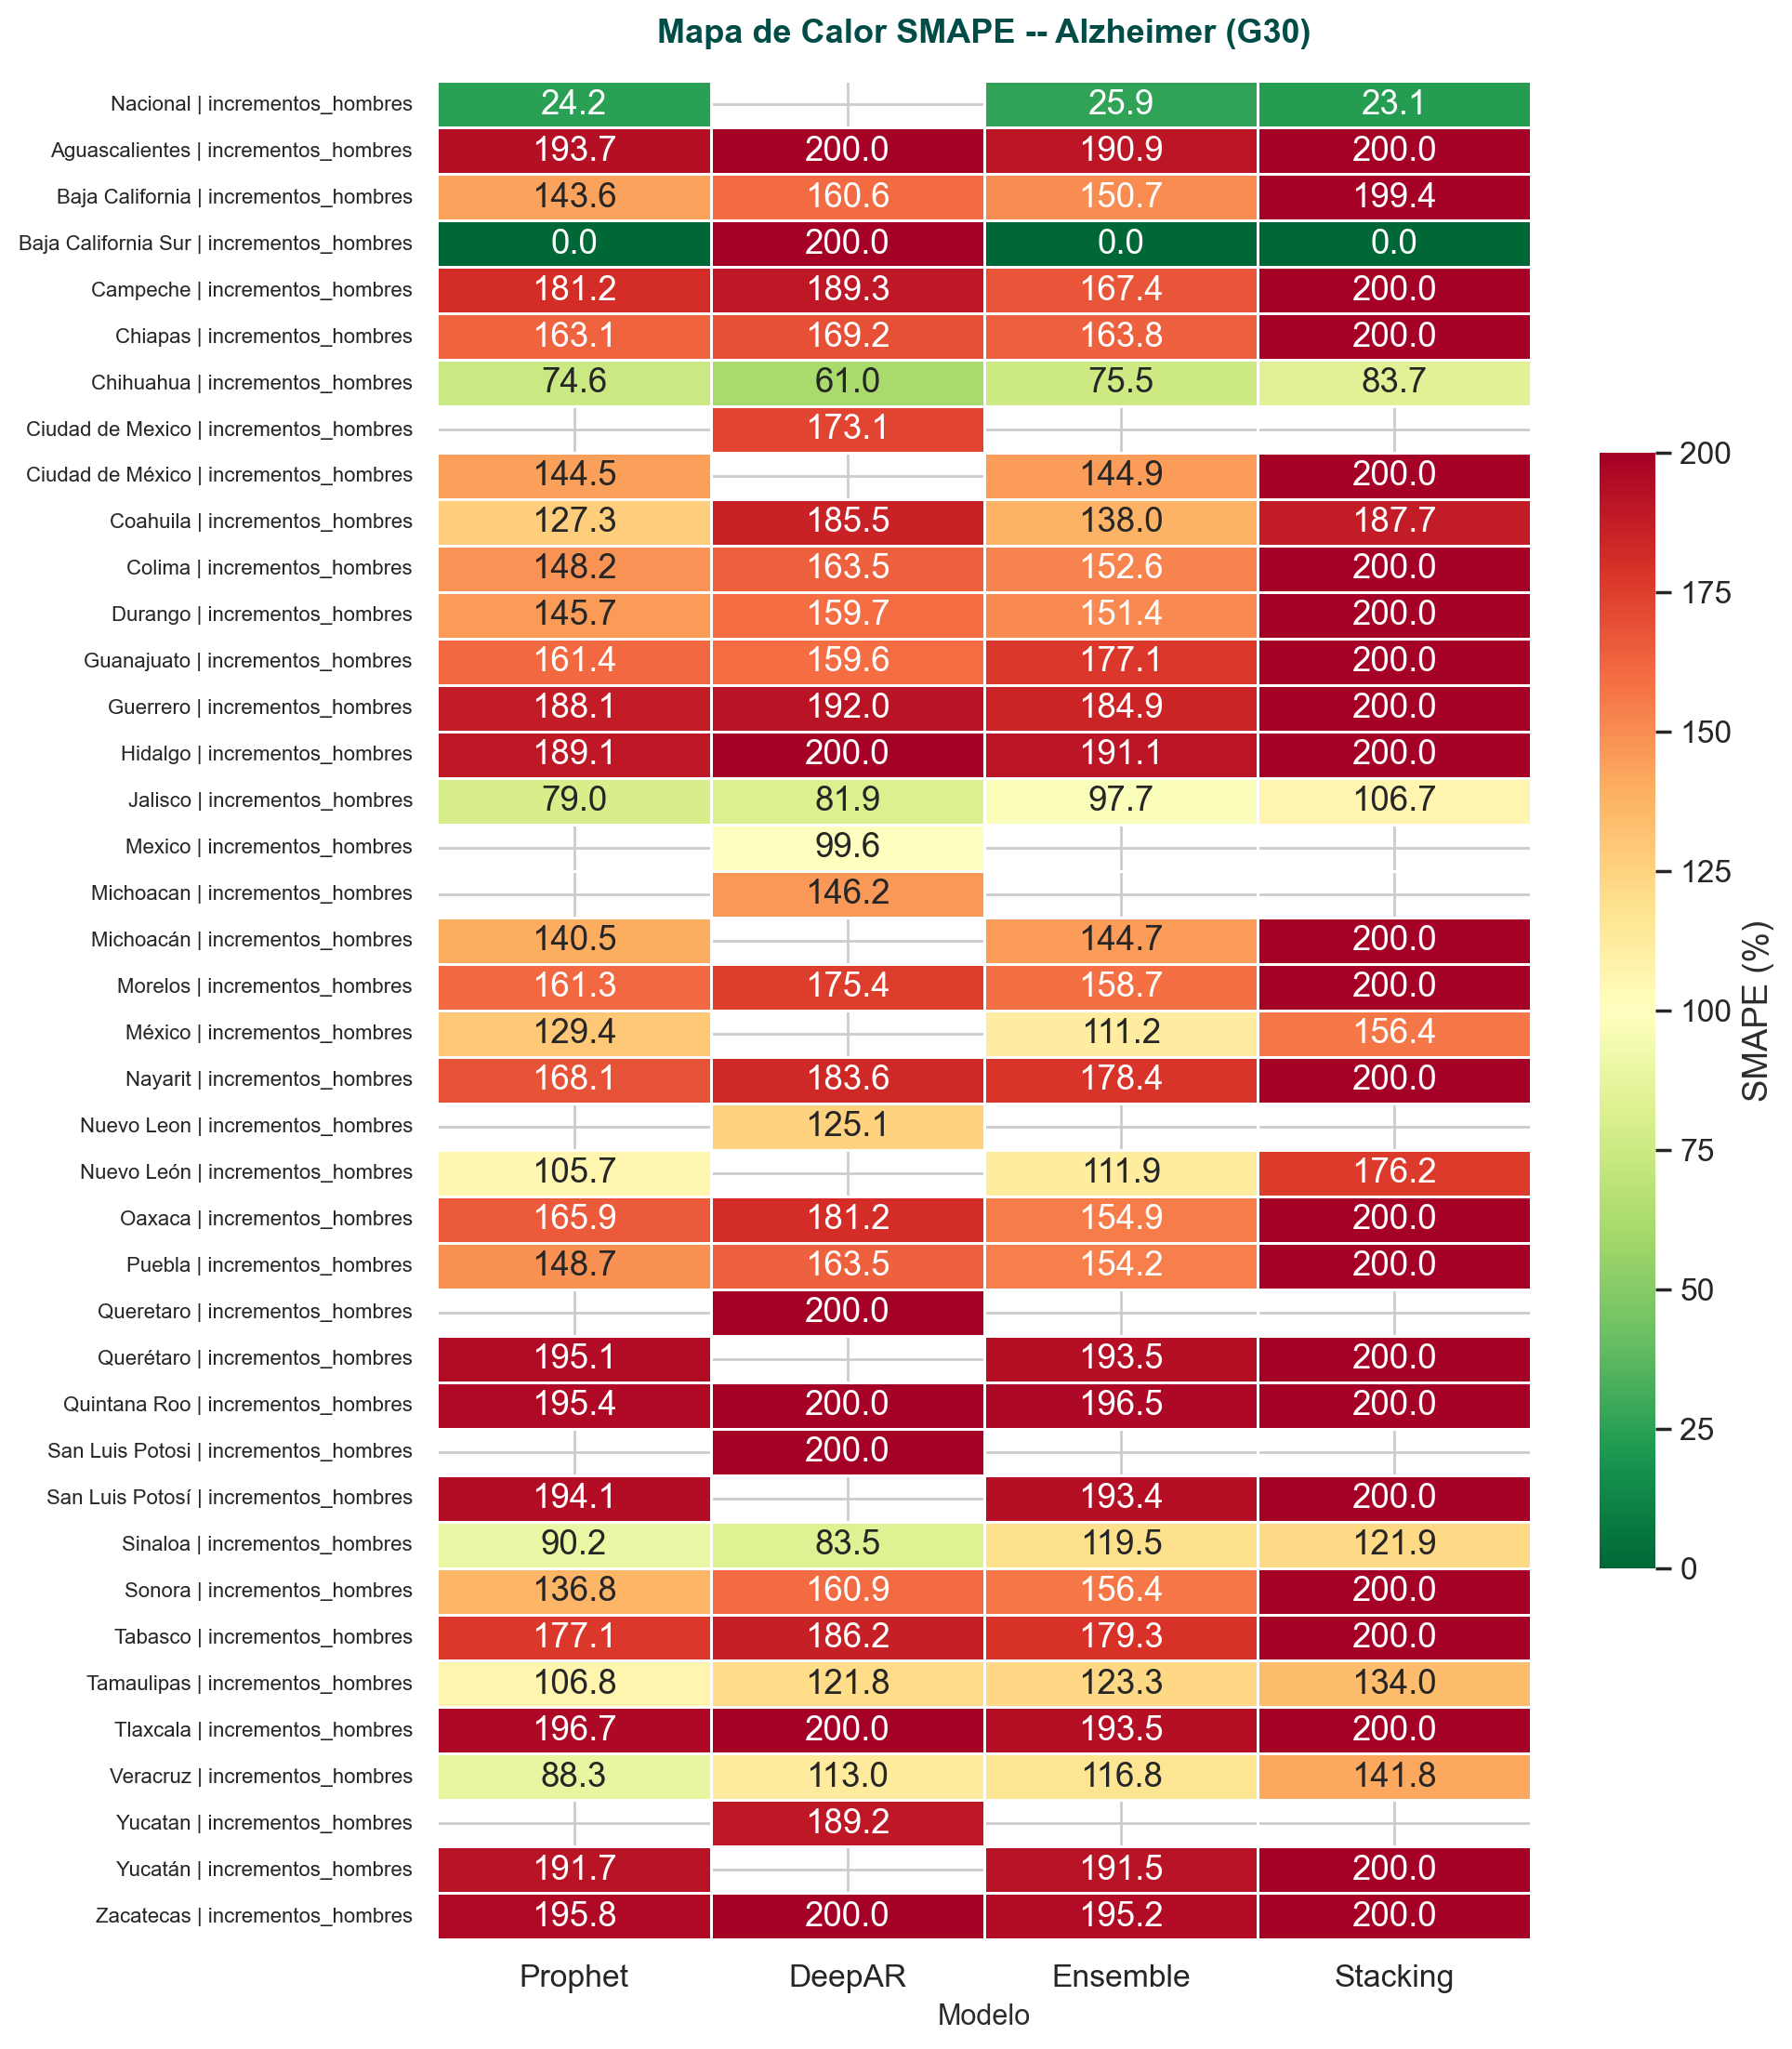
\includegraphics[width=0.85\textwidth]{figuras_avance5/17_heatmap_smape_alzheimer.png}
    \caption{Mapa de calor SMAPE por entidad: Alzheimer. El rojo predomina por la inflación matemática del SMAPE con valores cercanos a cero. El MASE $<1.0$ confirma que los modelos superan al baseline naïve a pesar del SMAPE elevado.}
    \label{fig:heatmap_alz}
\end{figure}

\newpage

\subsection{Radar Multimétrica y Distribución de Errores}

% ---- FIGURAS: Radar y Violín ----
\begin{figure}[H]
    \centering
    \begin{subfigure}[t]{0.48\textwidth}
        \centering
        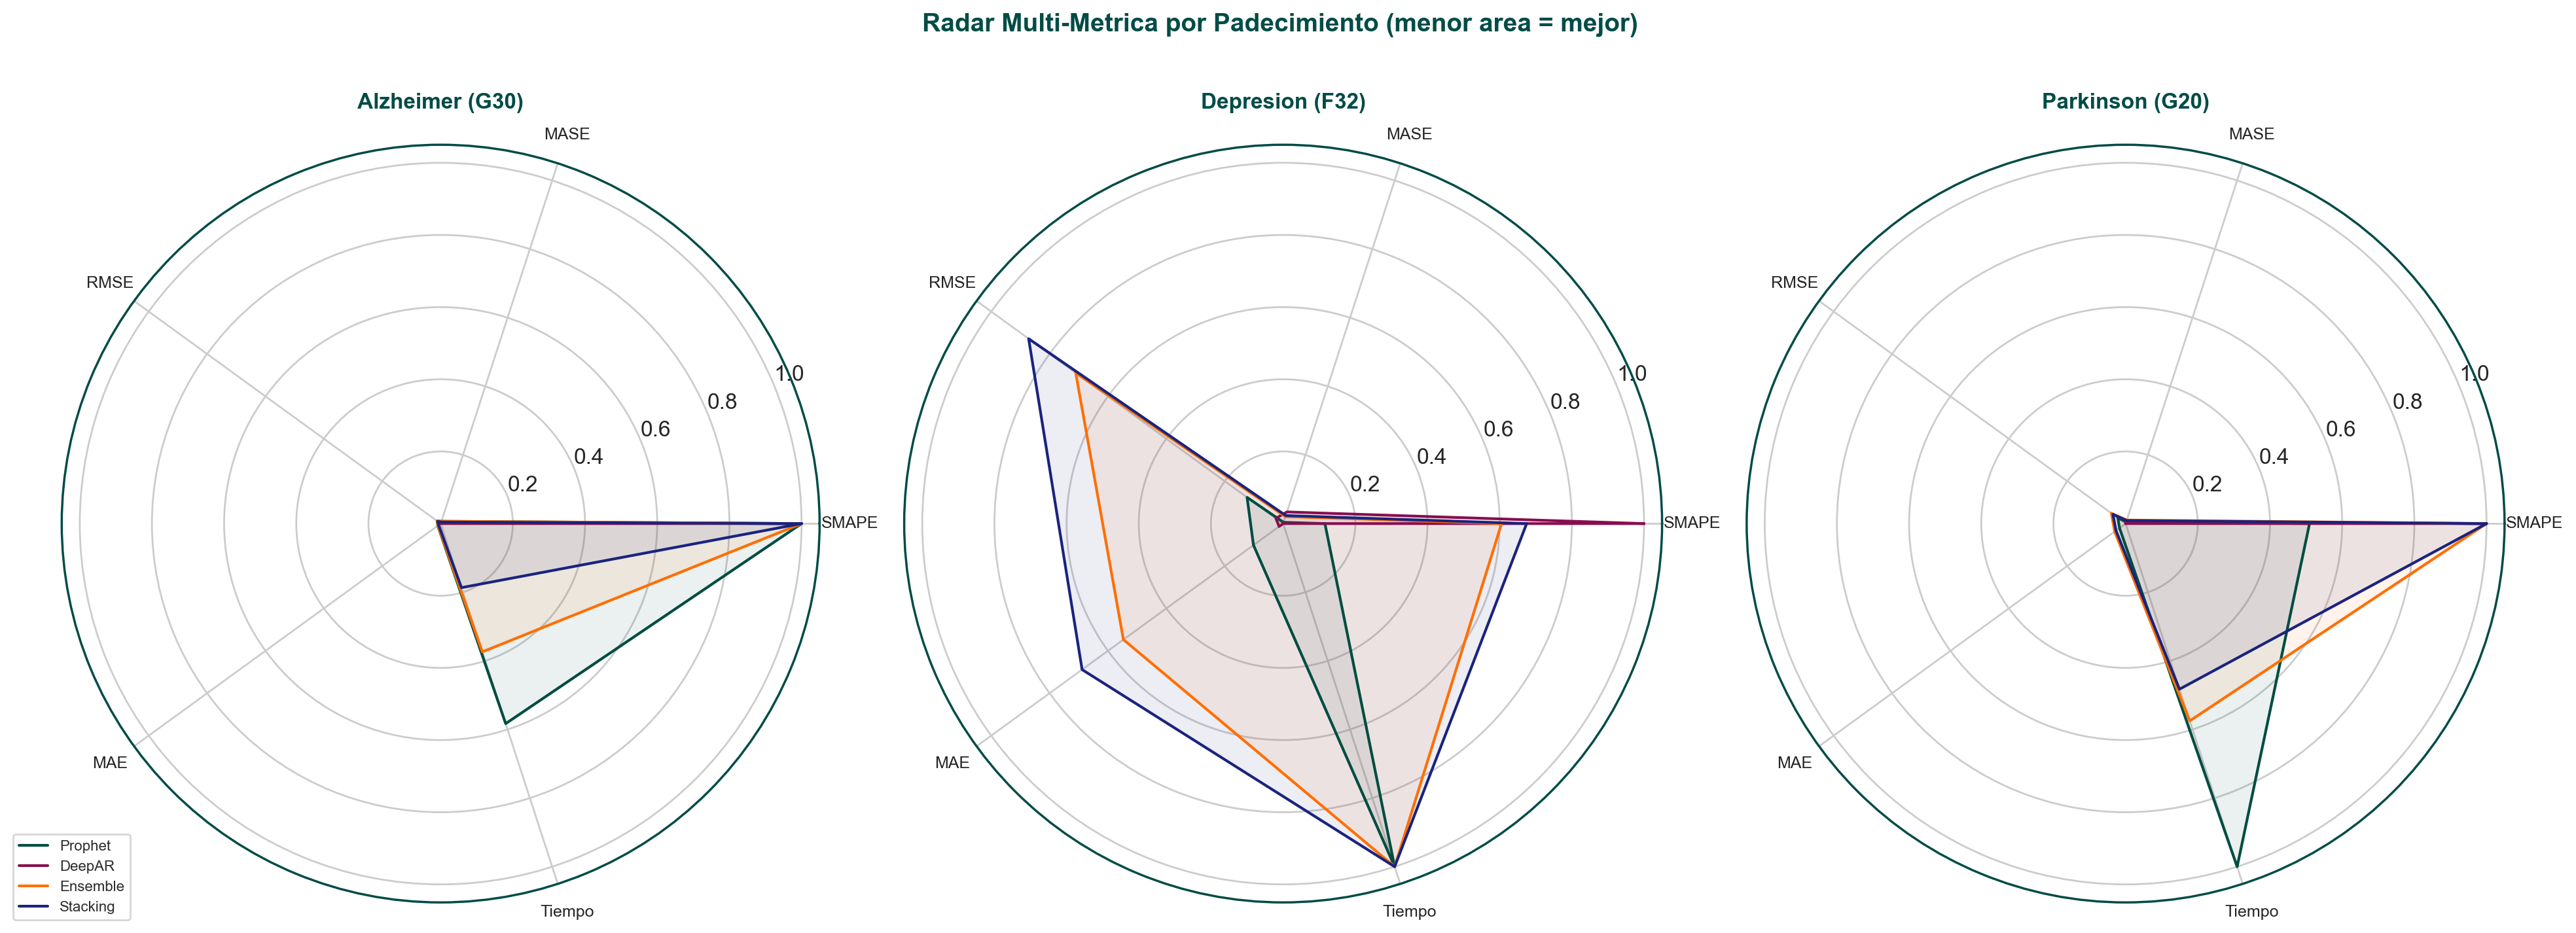
\includegraphics[width=\textwidth]{figuras_avance5/13_radar_multimetrica.png}
        \caption{Radar multimétrica: cada eje representa una métrica normalizada. El área menor indica mejor desempeño.}
        \label{fig:radar}
    \end{subfigure}
    \hfill
    \begin{subfigure}[t]{0.48\textwidth}
        \centering
        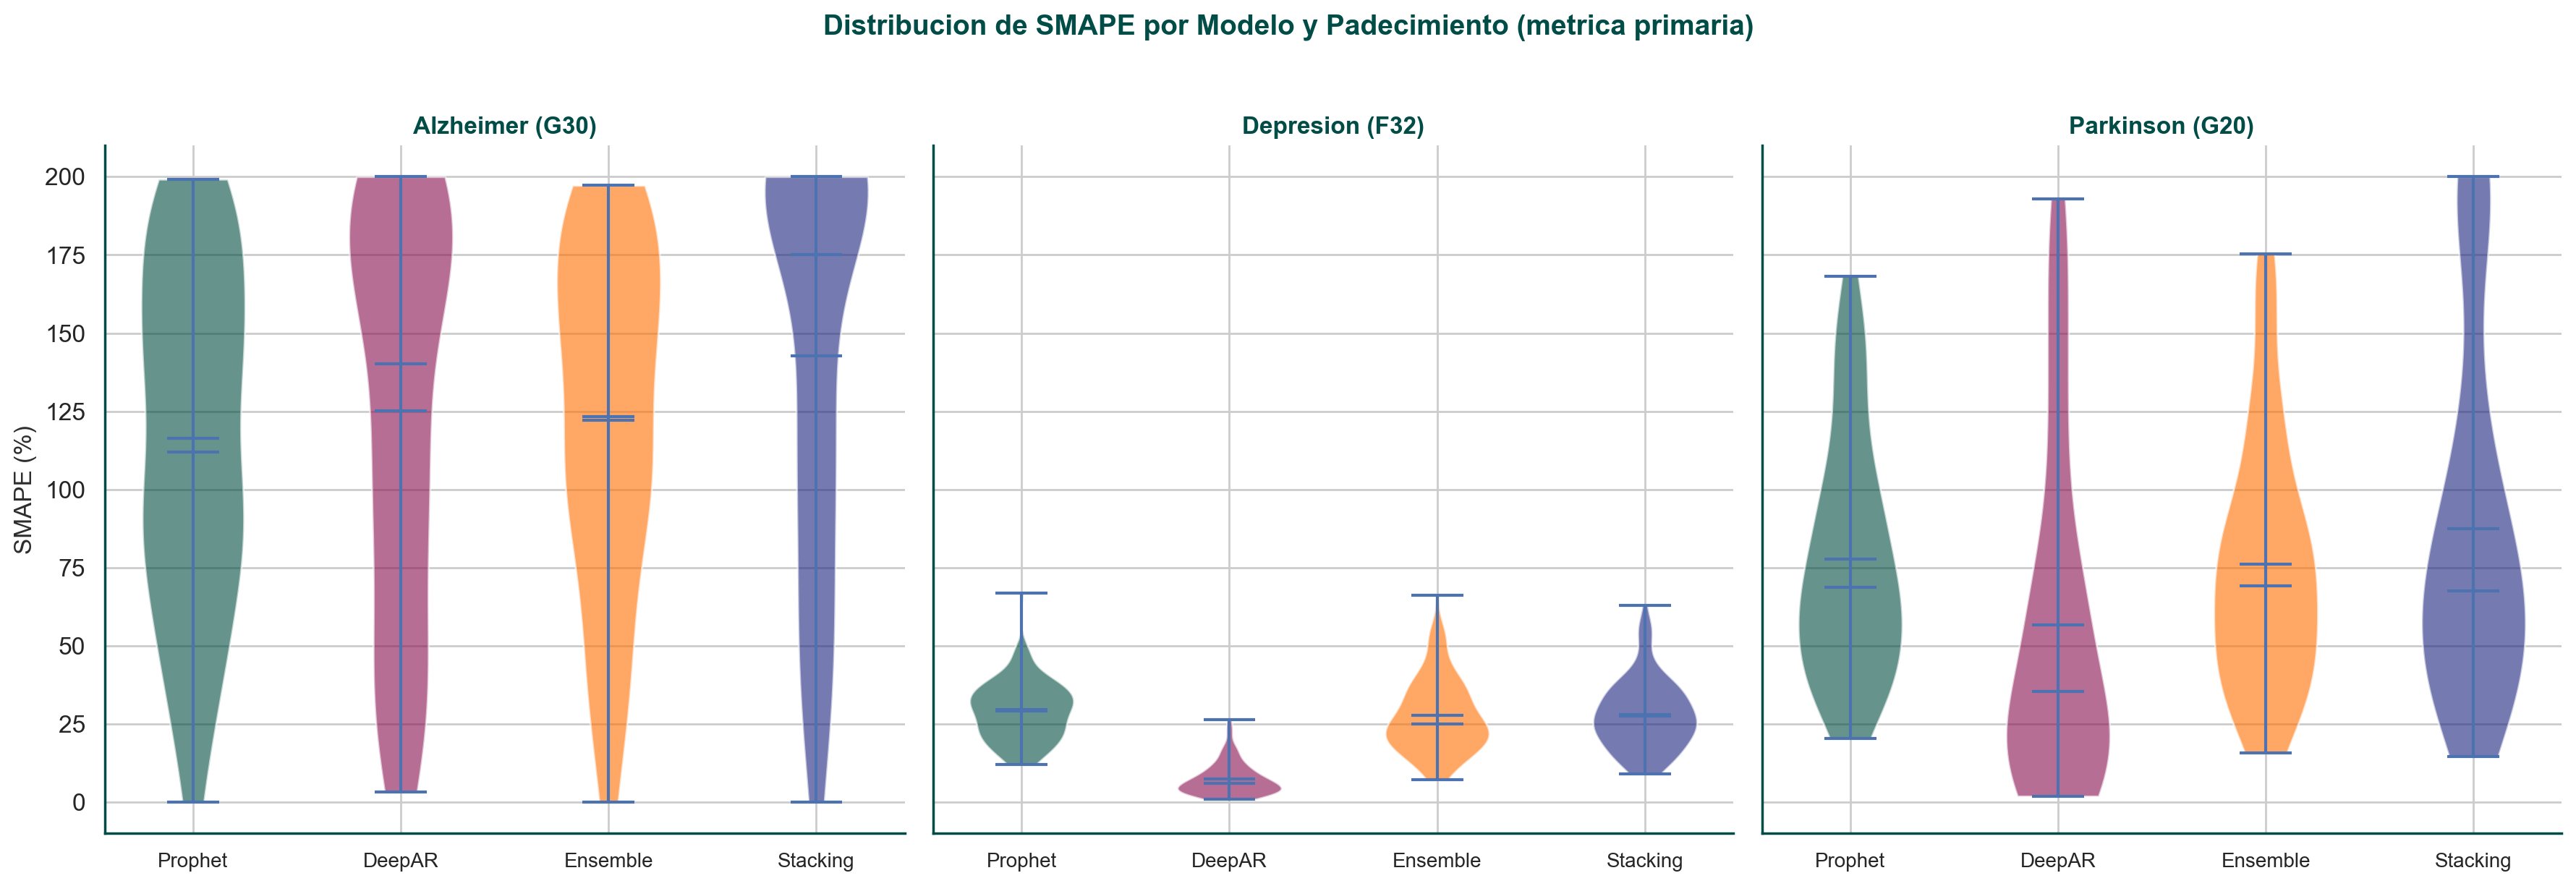
\includegraphics[width=\textwidth]{figuras_avance5/14_violin_smape.png}
        \caption{Distribución (violín) del SMAPE por motor. DeepAR tiene la cola inferior más concentrada.}
        \label{fig:violin}
    \end{subfigure}
    \caption{Comparativa visual de desempeño entre los 4 motores.}
    \label{fig:radar_violin}
\end{figure}

\subsection{Pesos de Ensamble y Producción}

% ---- FIGURAS: Pesos y Donut ----
\begin{figure}[H]
    \centering
    \begin{subfigure}[t]{0.48\textwidth}
        \centering
        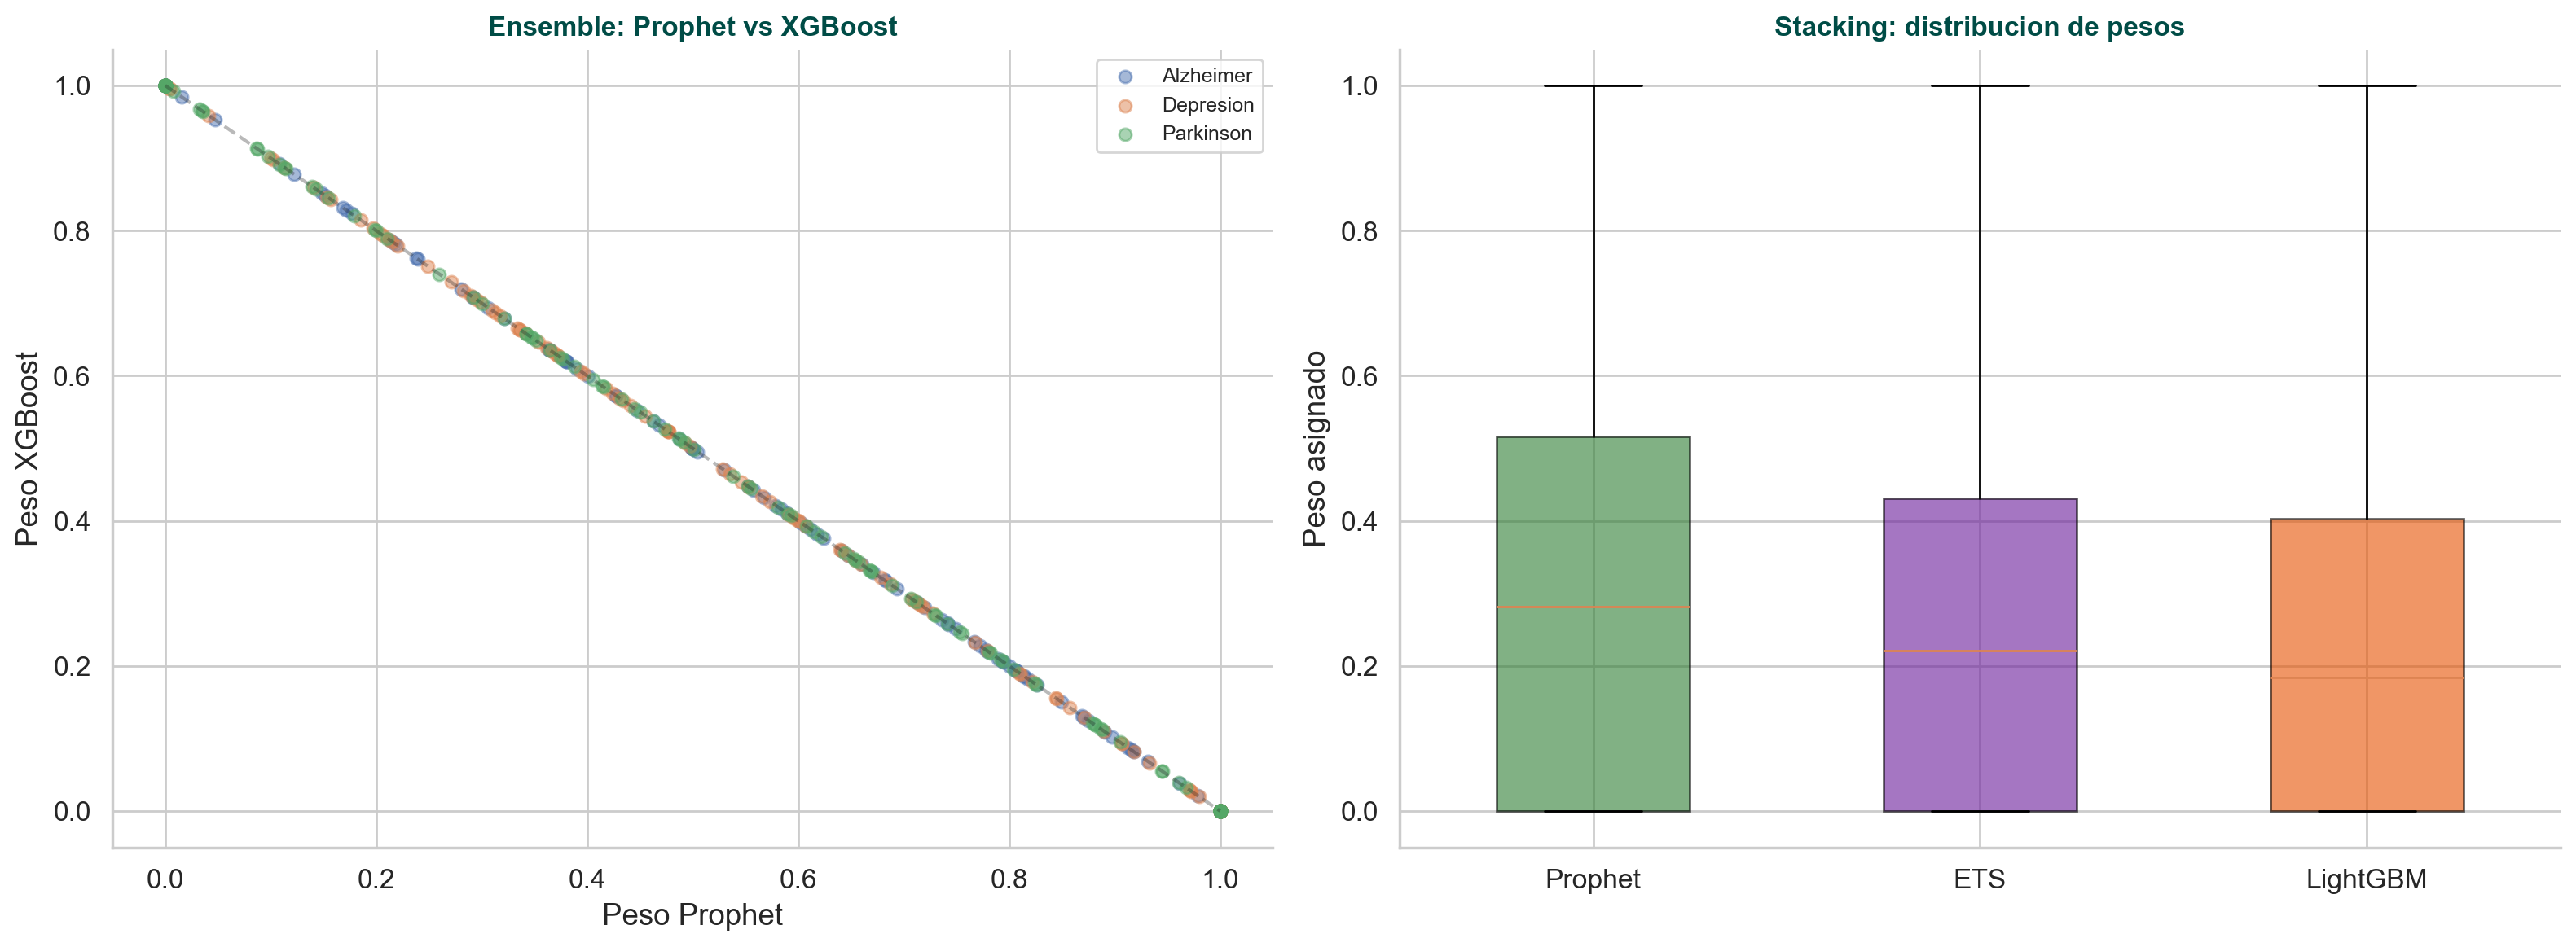
\includegraphics[width=\textwidth]{figuras_avance5/11_pesos_ensemble_stacking.png}
        \caption{Pesos aprendidos de Ensemble (Ridge) y Stacking (ElasticNet) por padecimiento.}
        \label{fig:pesos}
    \end{subfigure}
    \hfill
    \begin{subfigure}[t]{0.48\textwidth}
        \centering
        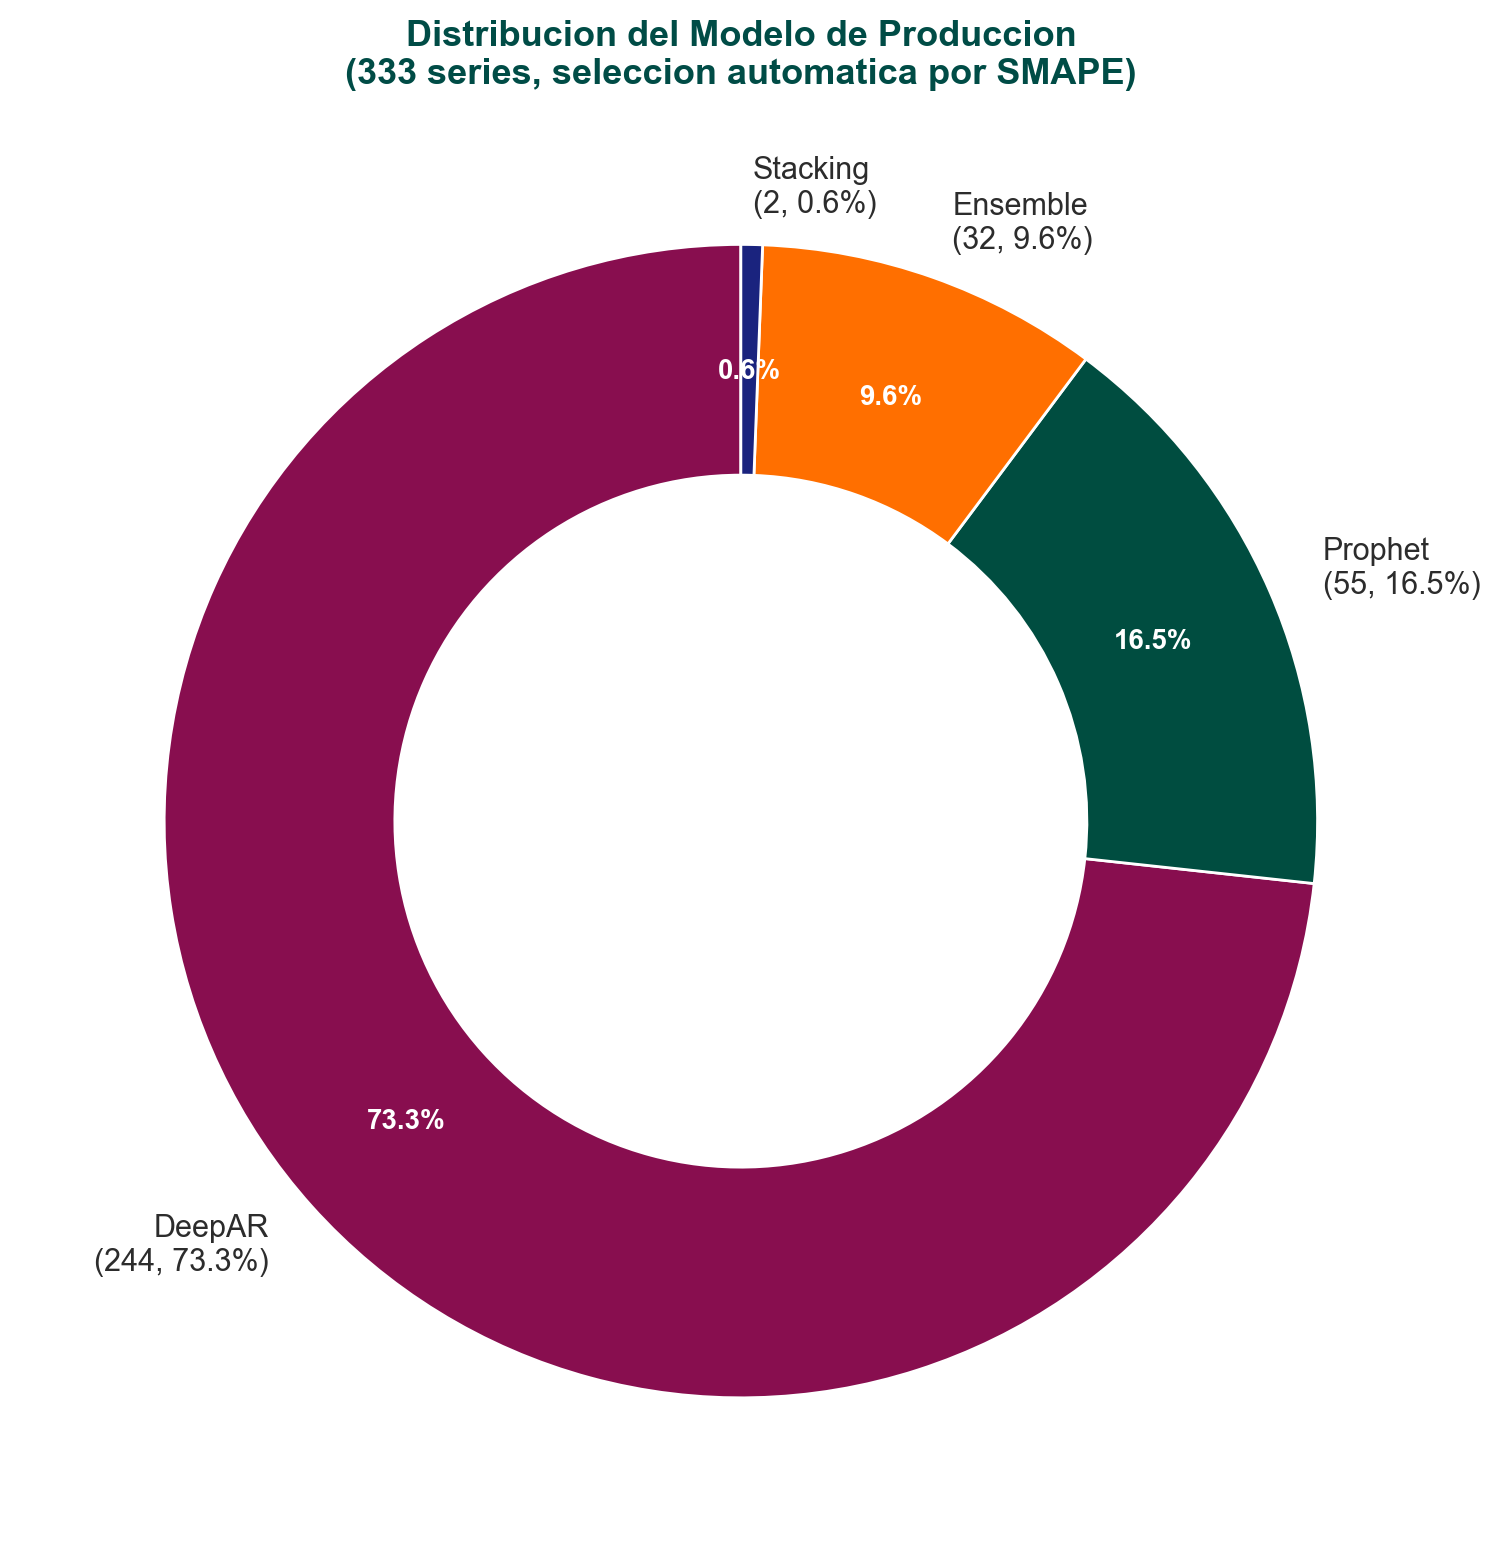
\includegraphics[width=\textwidth]{figuras_avance5/23_donut_produccion.png}
        \caption{Distribución del modelo ganador entre las 333 series de producción.}
        \label{fig:donut}
    \end{subfigure}
    \caption{Análisis de pesos y distribución de modelos en producción.}
    \label{fig:pesos_donut}
\end{figure}

% ---- FIGURAS: Scatter overfitting y Matriz ganador ----
\begin{figure}[H]
    \centering
    \begin{subfigure}[t]{0.48\textwidth}
        \centering
        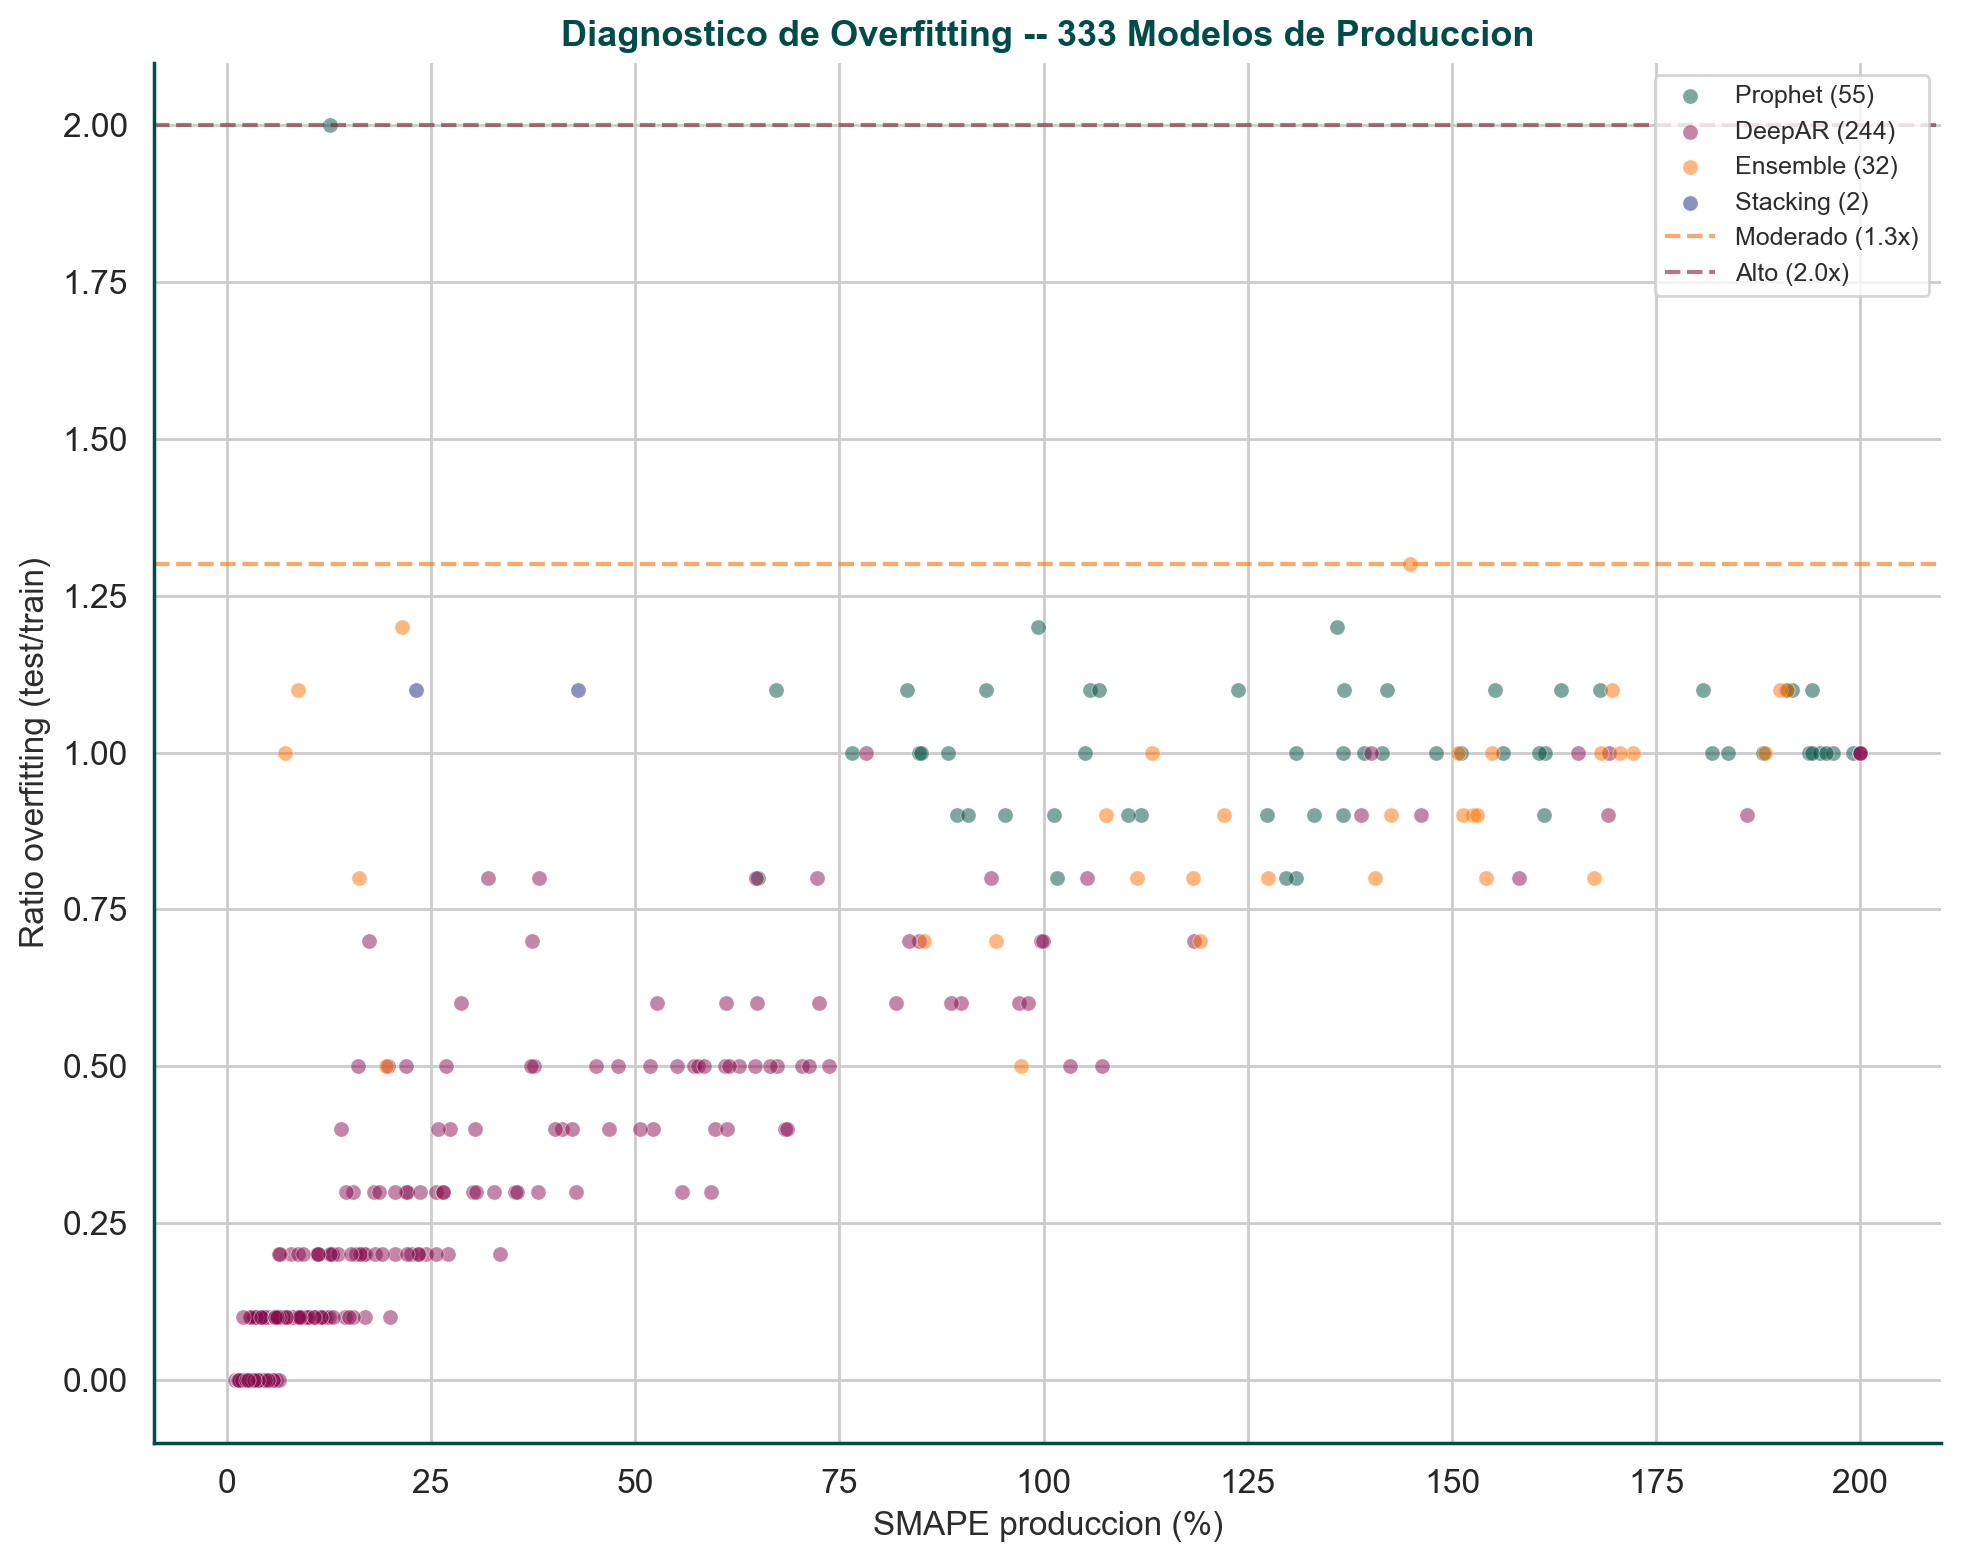
\includegraphics[width=\textwidth]{figuras_avance5/25_scatter_overfitting.png}
        \caption{Scatter de SMAPE test vs.\ train. Los puntos cerca de la diagonal indican ausencia de sobreajuste.}
        \label{fig:scatter_overfit}
    \end{subfigure}
    \hfill
    \begin{subfigure}[t]{0.48\textwidth}
        \centering
        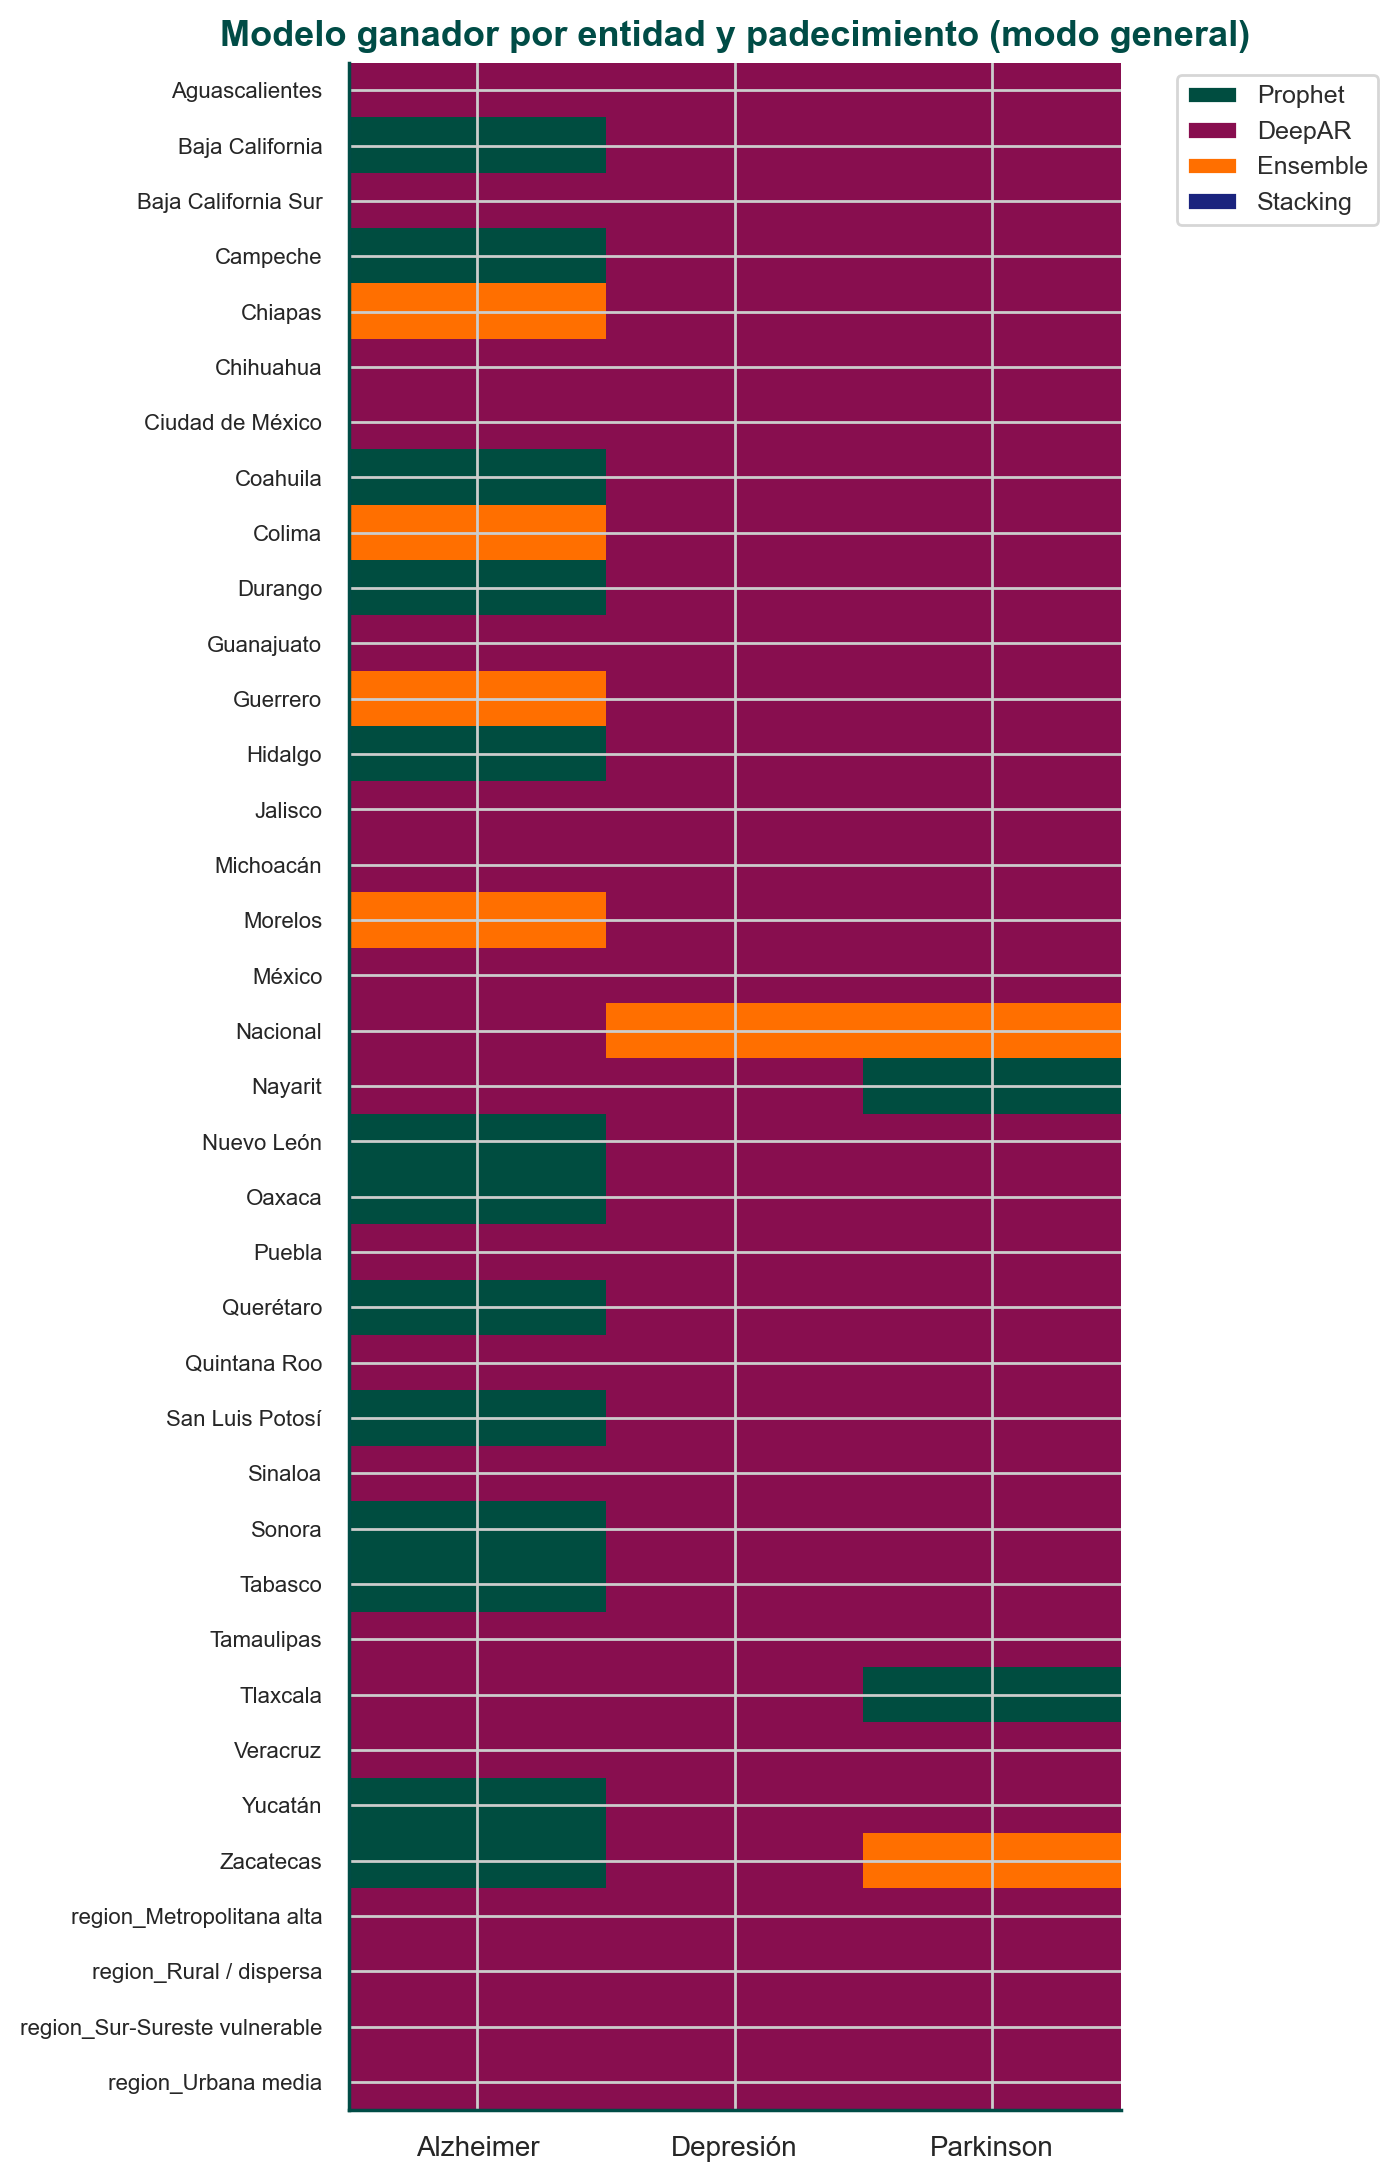
\includegraphics[width=\textwidth]{figuras_avance5/32_matriz_ganador.png}
        \caption{Matriz de frecuencia del modelo ganador por padecimiento y entidad.}
        \label{fig:matriz_ganador}
    \end{subfigure}
    \caption{Diagnósticos de overfitting y selección de producción.}
    \label{fig:overfit_matriz}
\end{figure}

\newpage

\subsection{Gráficos Adicionales de Interpretabilidad}

% ---- FIGURAS: Hiperparámetros y Seasonality ----
\begin{figure}[H]
    \centering
    \begin{subfigure}[t]{0.48\textwidth}
        \centering
        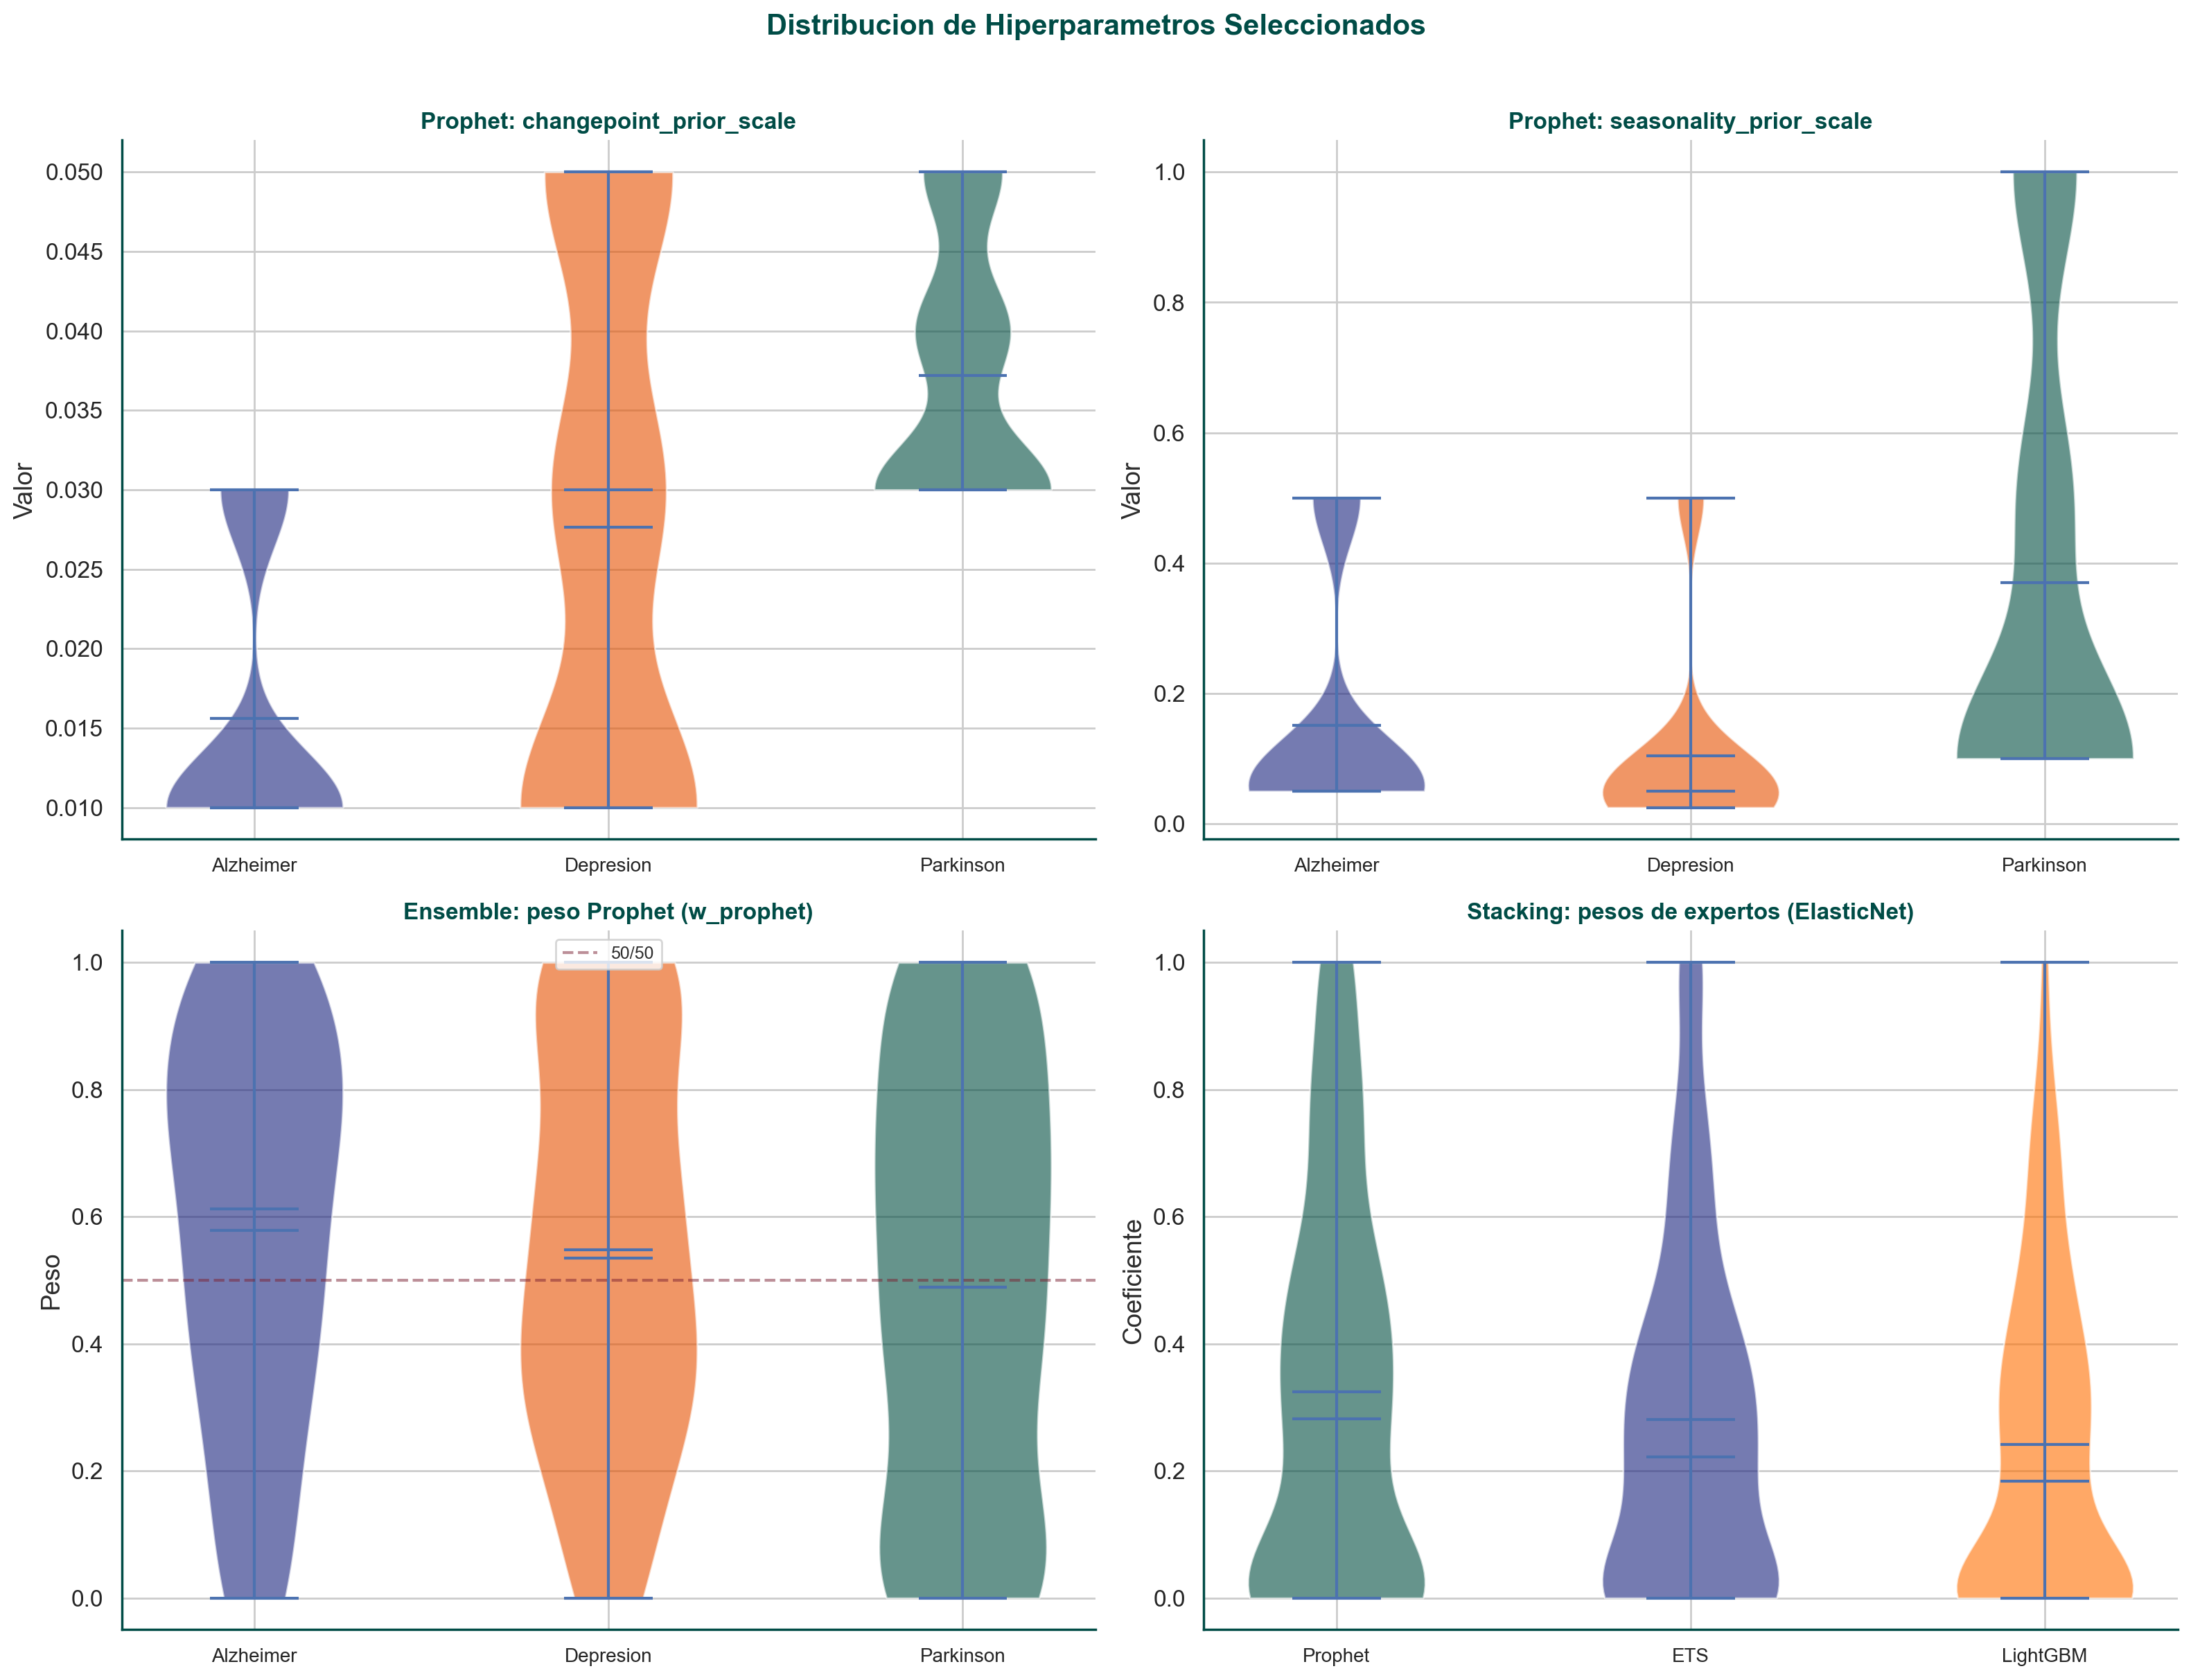
\includegraphics[width=\textwidth]{figuras_avance5/08_violin_hiperparametros.png}
        \caption{Distribución de hiperparámetros óptimos de Prophet (violin plot).}
        \label{fig:violin_hp}
    \end{subfigure}
    \hfill
    \begin{subfigure}[t]{0.48\textwidth}
        \centering
        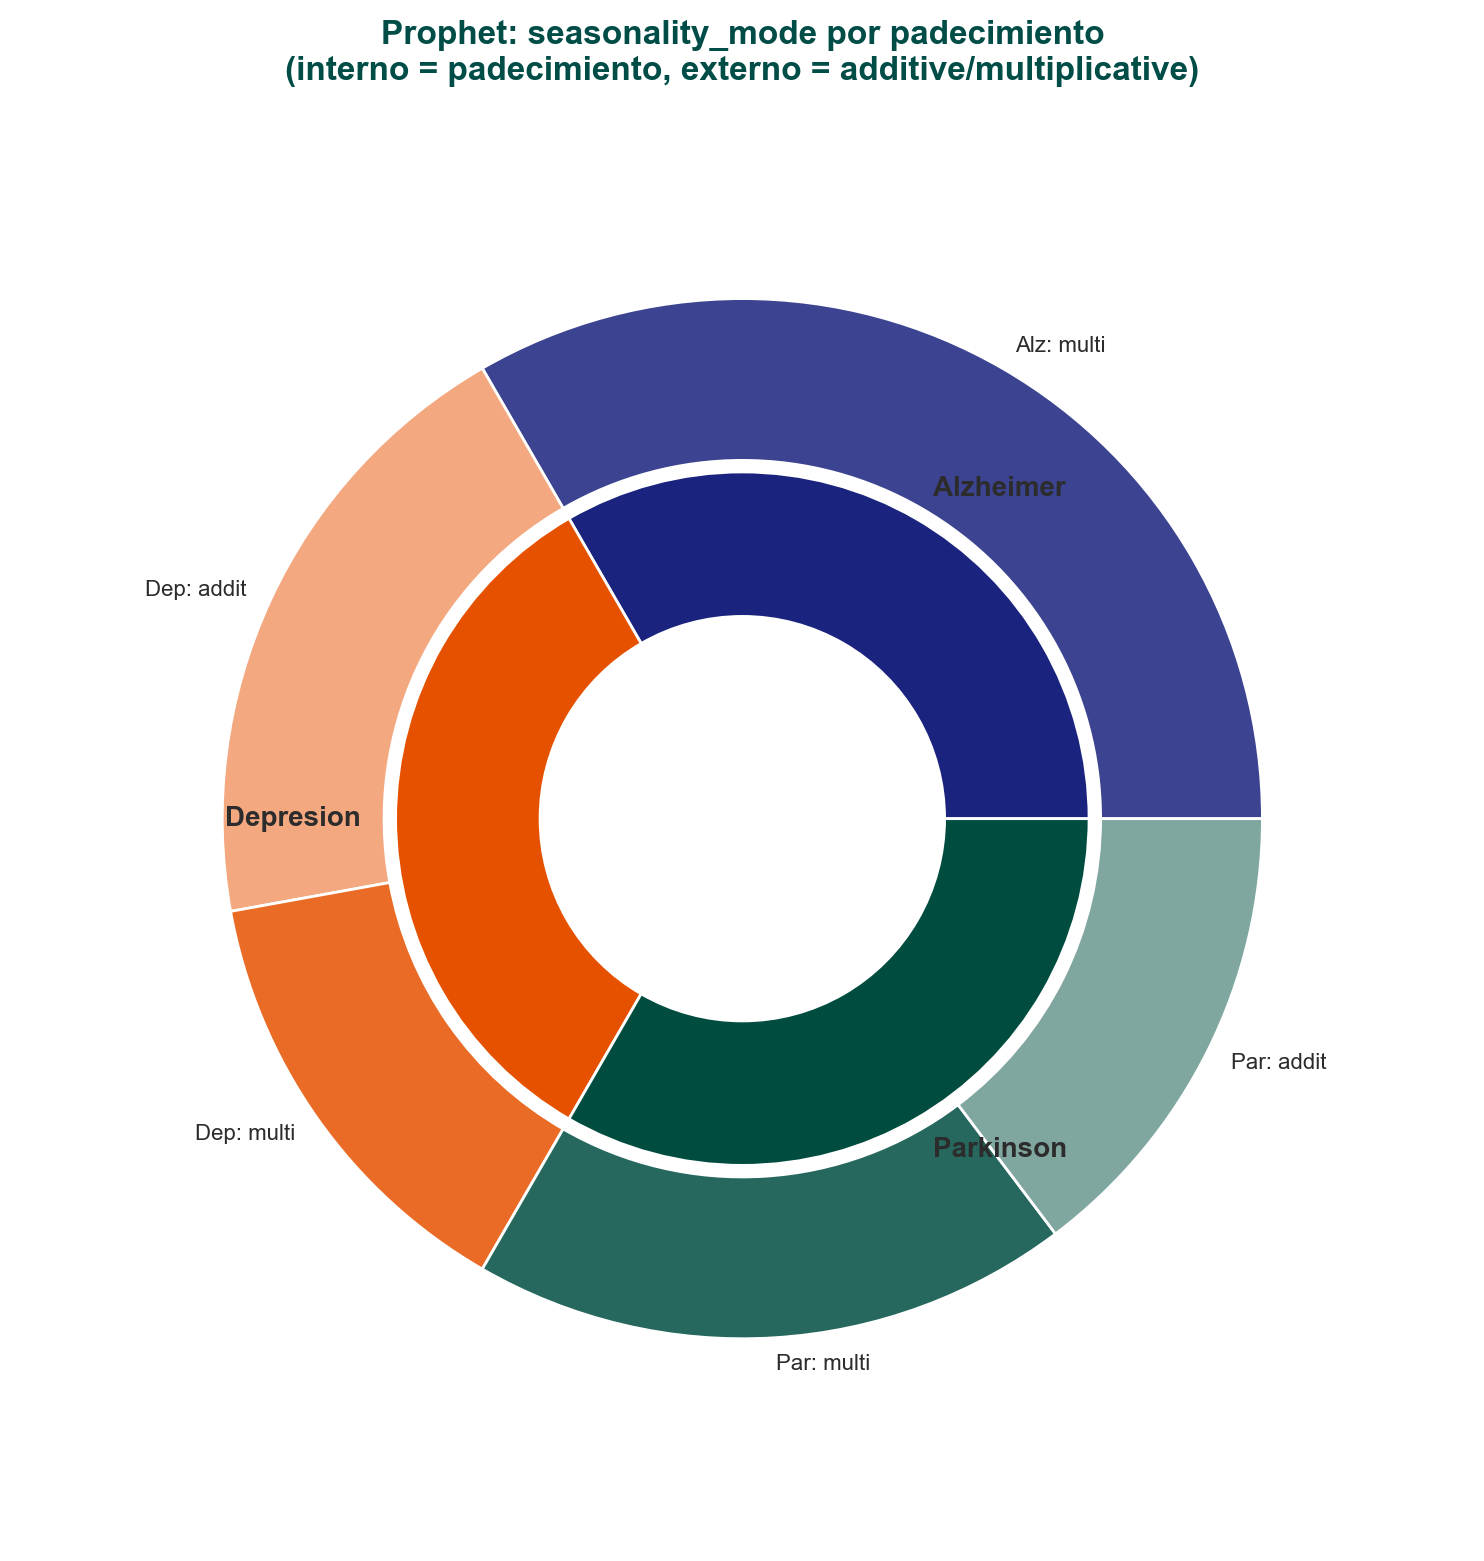
\includegraphics[width=\textwidth]{figuras_avance5/09_donut_seasonality.png}
        \caption{Modo de estacionalidad seleccionado: 65.8\,\% multiplicativo vs.\ 34.2\,\% aditivo.}
        \label{fig:donut_season}
    \end{subfigure}
    \caption{Análisis de hiperparámetros de Prophet sobre los 333 modelos.}
    \label{fig:hp_season}
\end{figure}

% ---- FIGURAS: Ternario, Stacking coefs, Frontera ----
\begin{figure}[H]
    \centering
    \begin{subfigure}[t]{0.48\textwidth}
        \centering
        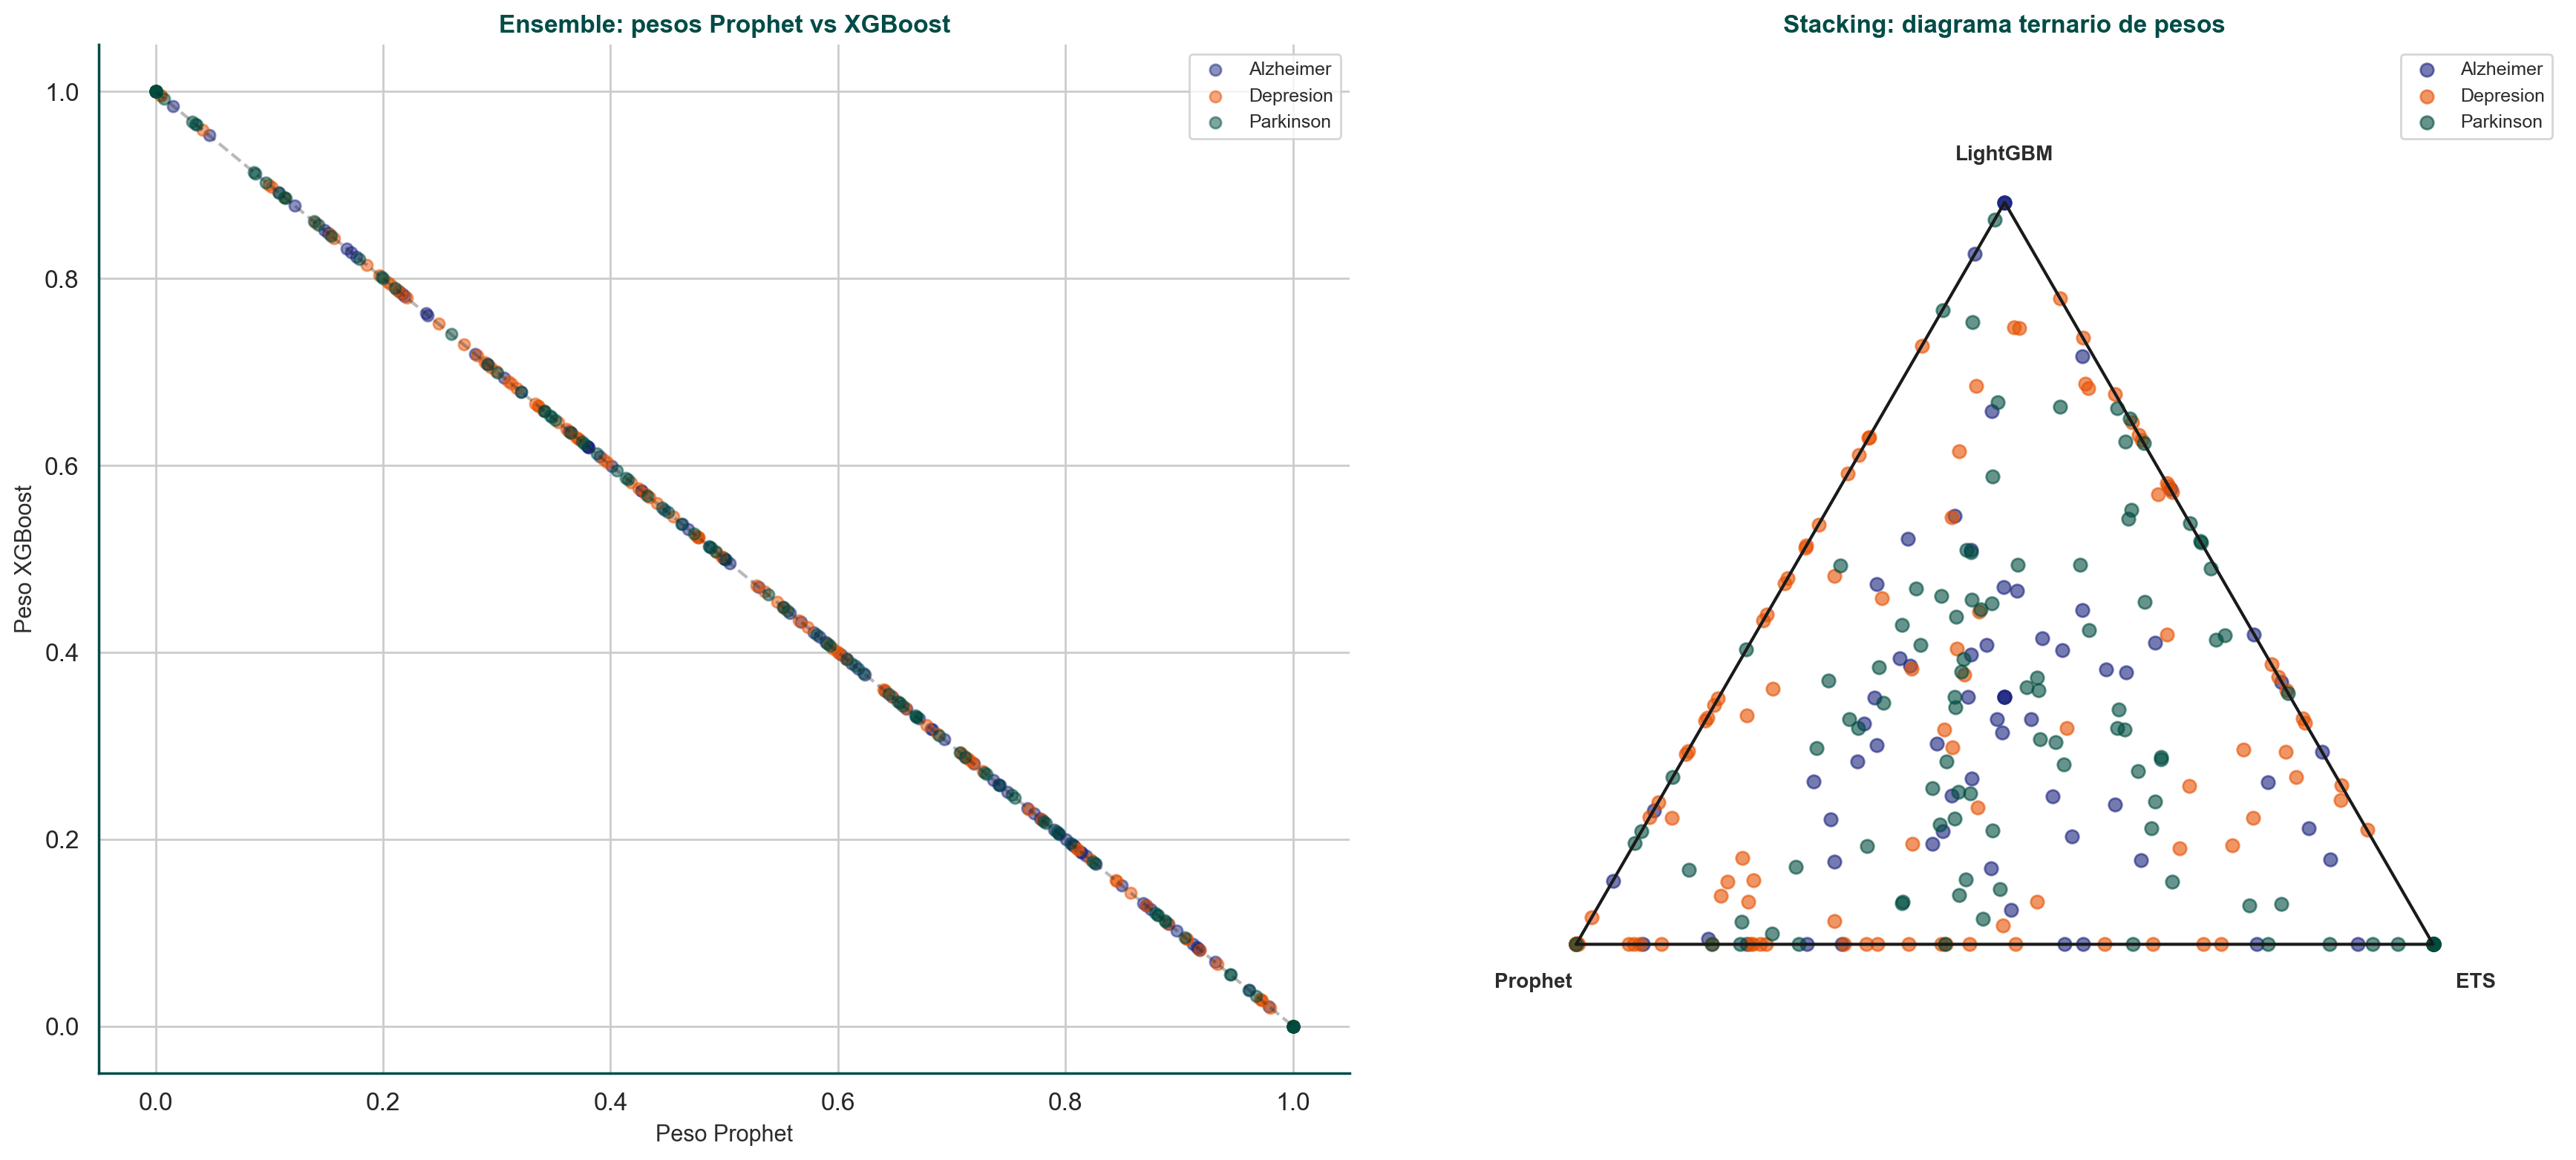
\includegraphics[width=\textwidth]{figuras_avance5/18_ternario_pesos.png}
        \caption{Diagrama ternario de pesos del Stacking (Prophet/ETS/LightGBM).}
        \label{fig:ternario}
    \end{subfigure}
    \hfill
    \begin{subfigure}[t]{0.48\textwidth}
        \centering
        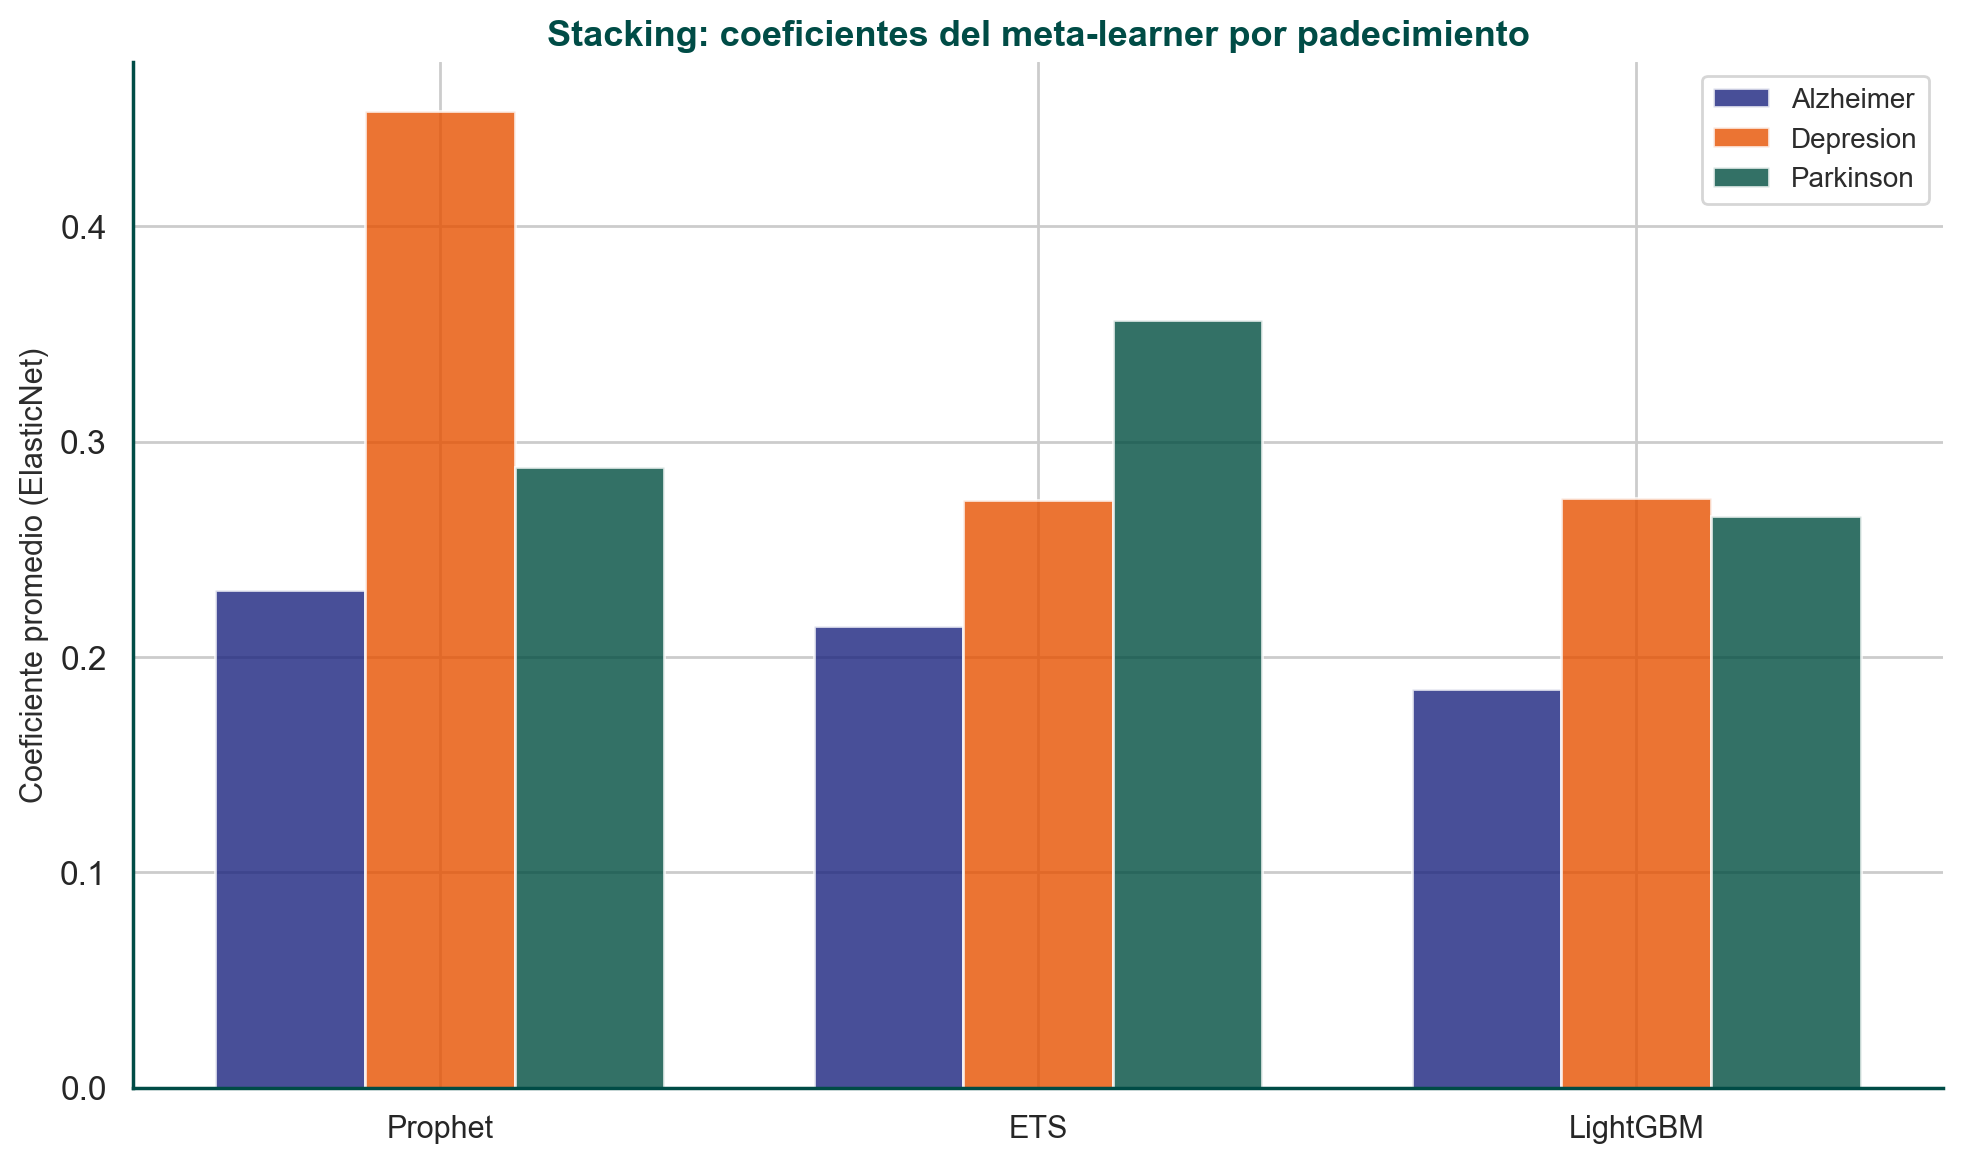
\includegraphics[width=\textwidth]{figuras_avance5/20_stacking_coeficientes.png}
        \caption{Coeficientes del meta-learner ElasticNet por serie.}
        \label{fig:stacking_coefs}
    \end{subfigure}
    \caption{Visualización de pesos del modelo Stacking.}
    \label{fig:stacking_viz}
\end{figure}

\begin{figure}[H]
    \centering
    \begin{subfigure}[t]{0.48\textwidth}
        \centering
        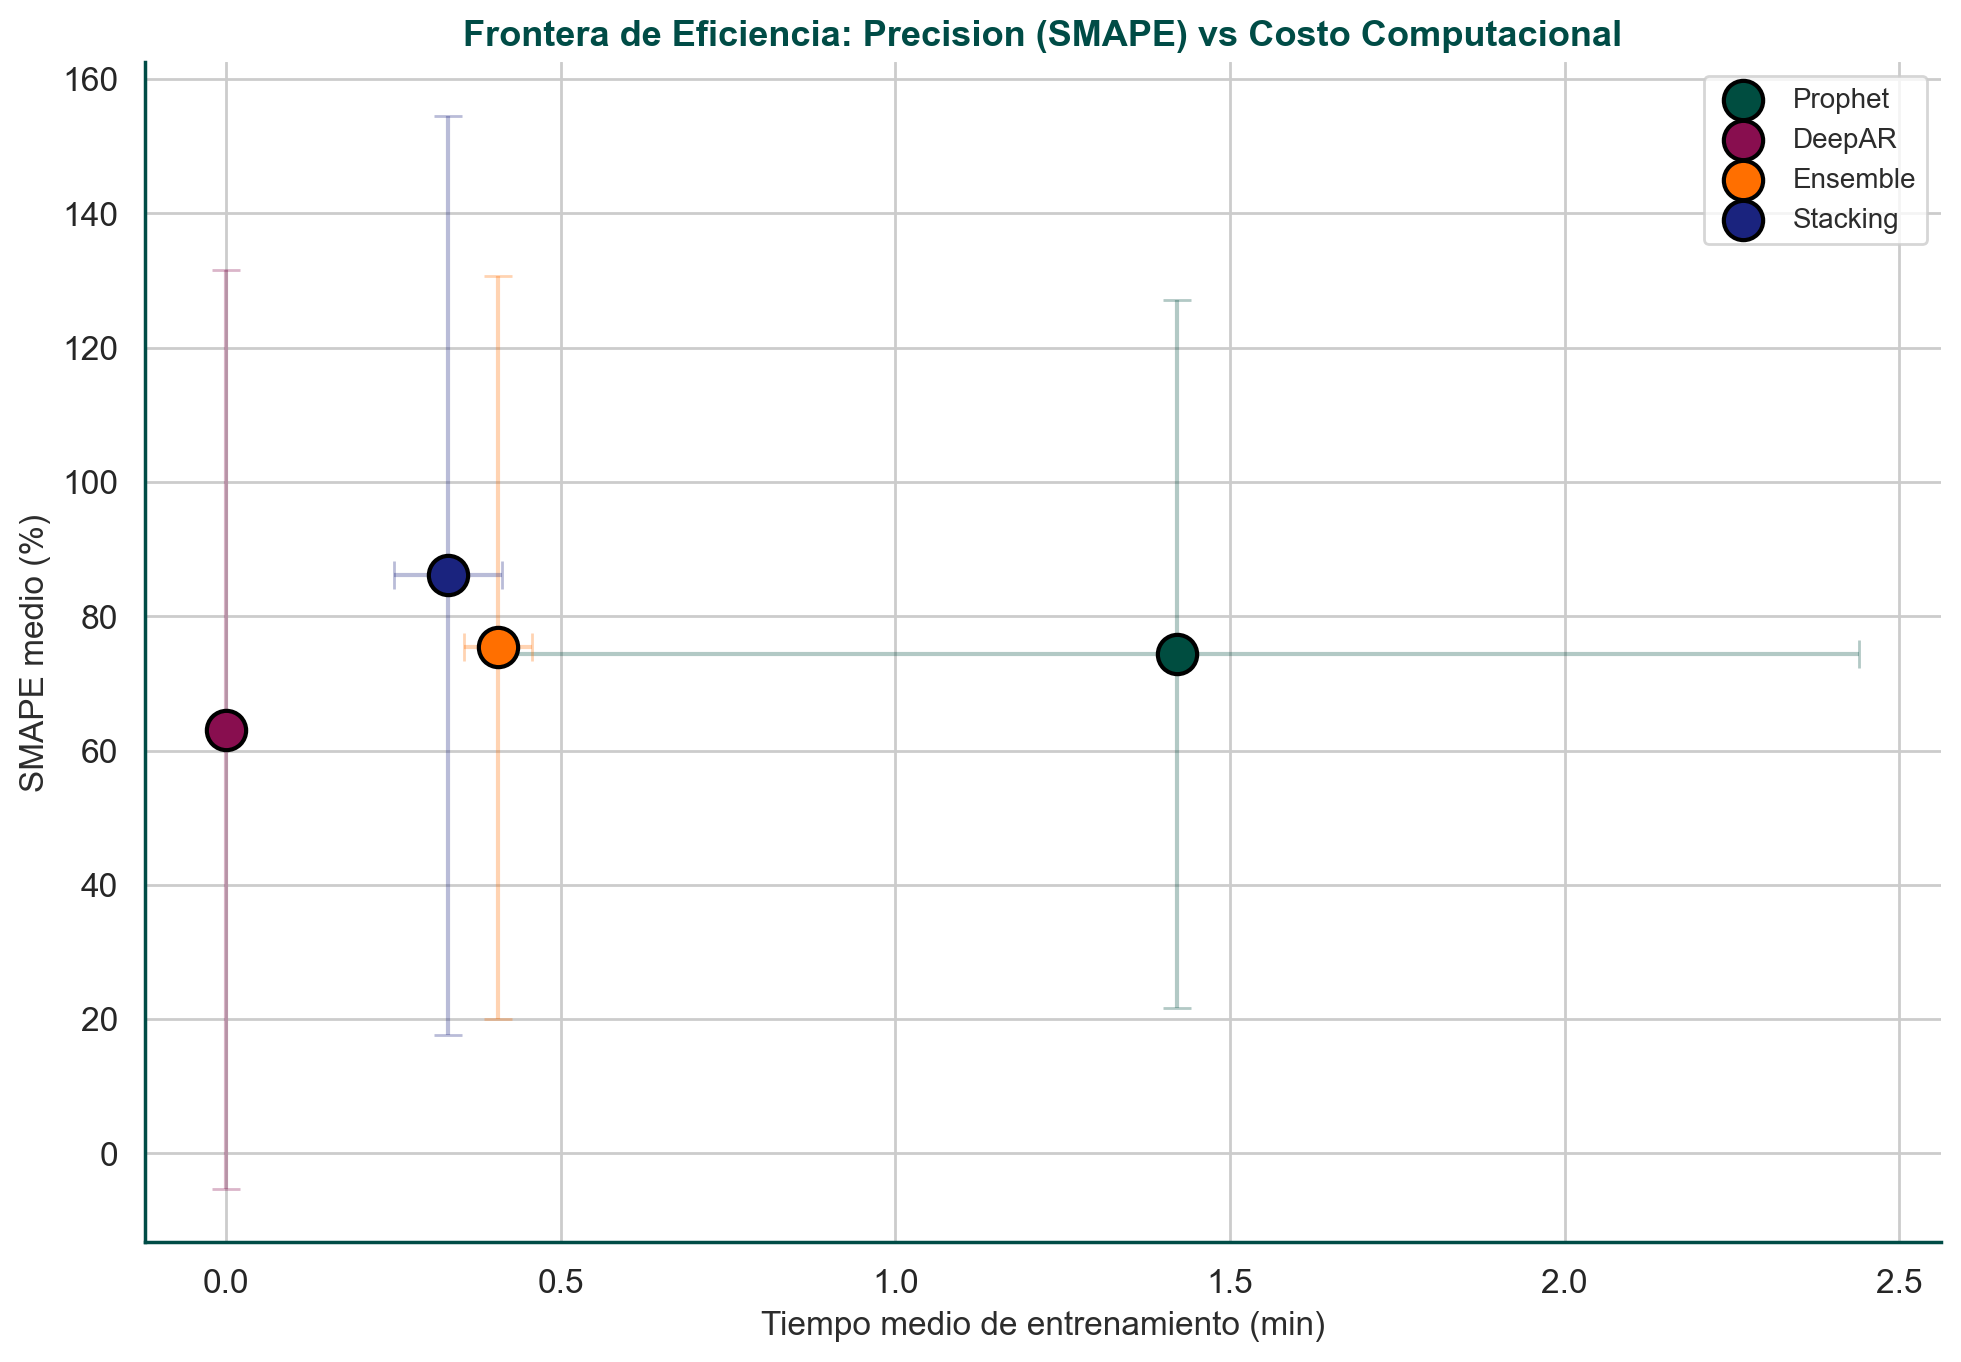
\includegraphics[width=\textwidth]{figuras_avance5/33_frontera_eficiencia.png}
        \caption{Frontera de eficiencia SMAPE vs.\ tiempo de entrenamiento.}
        \label{fig:frontera}
    \end{subfigure}
    \hfill
    \begin{subfigure}[t]{0.48\textwidth}
        \centering
        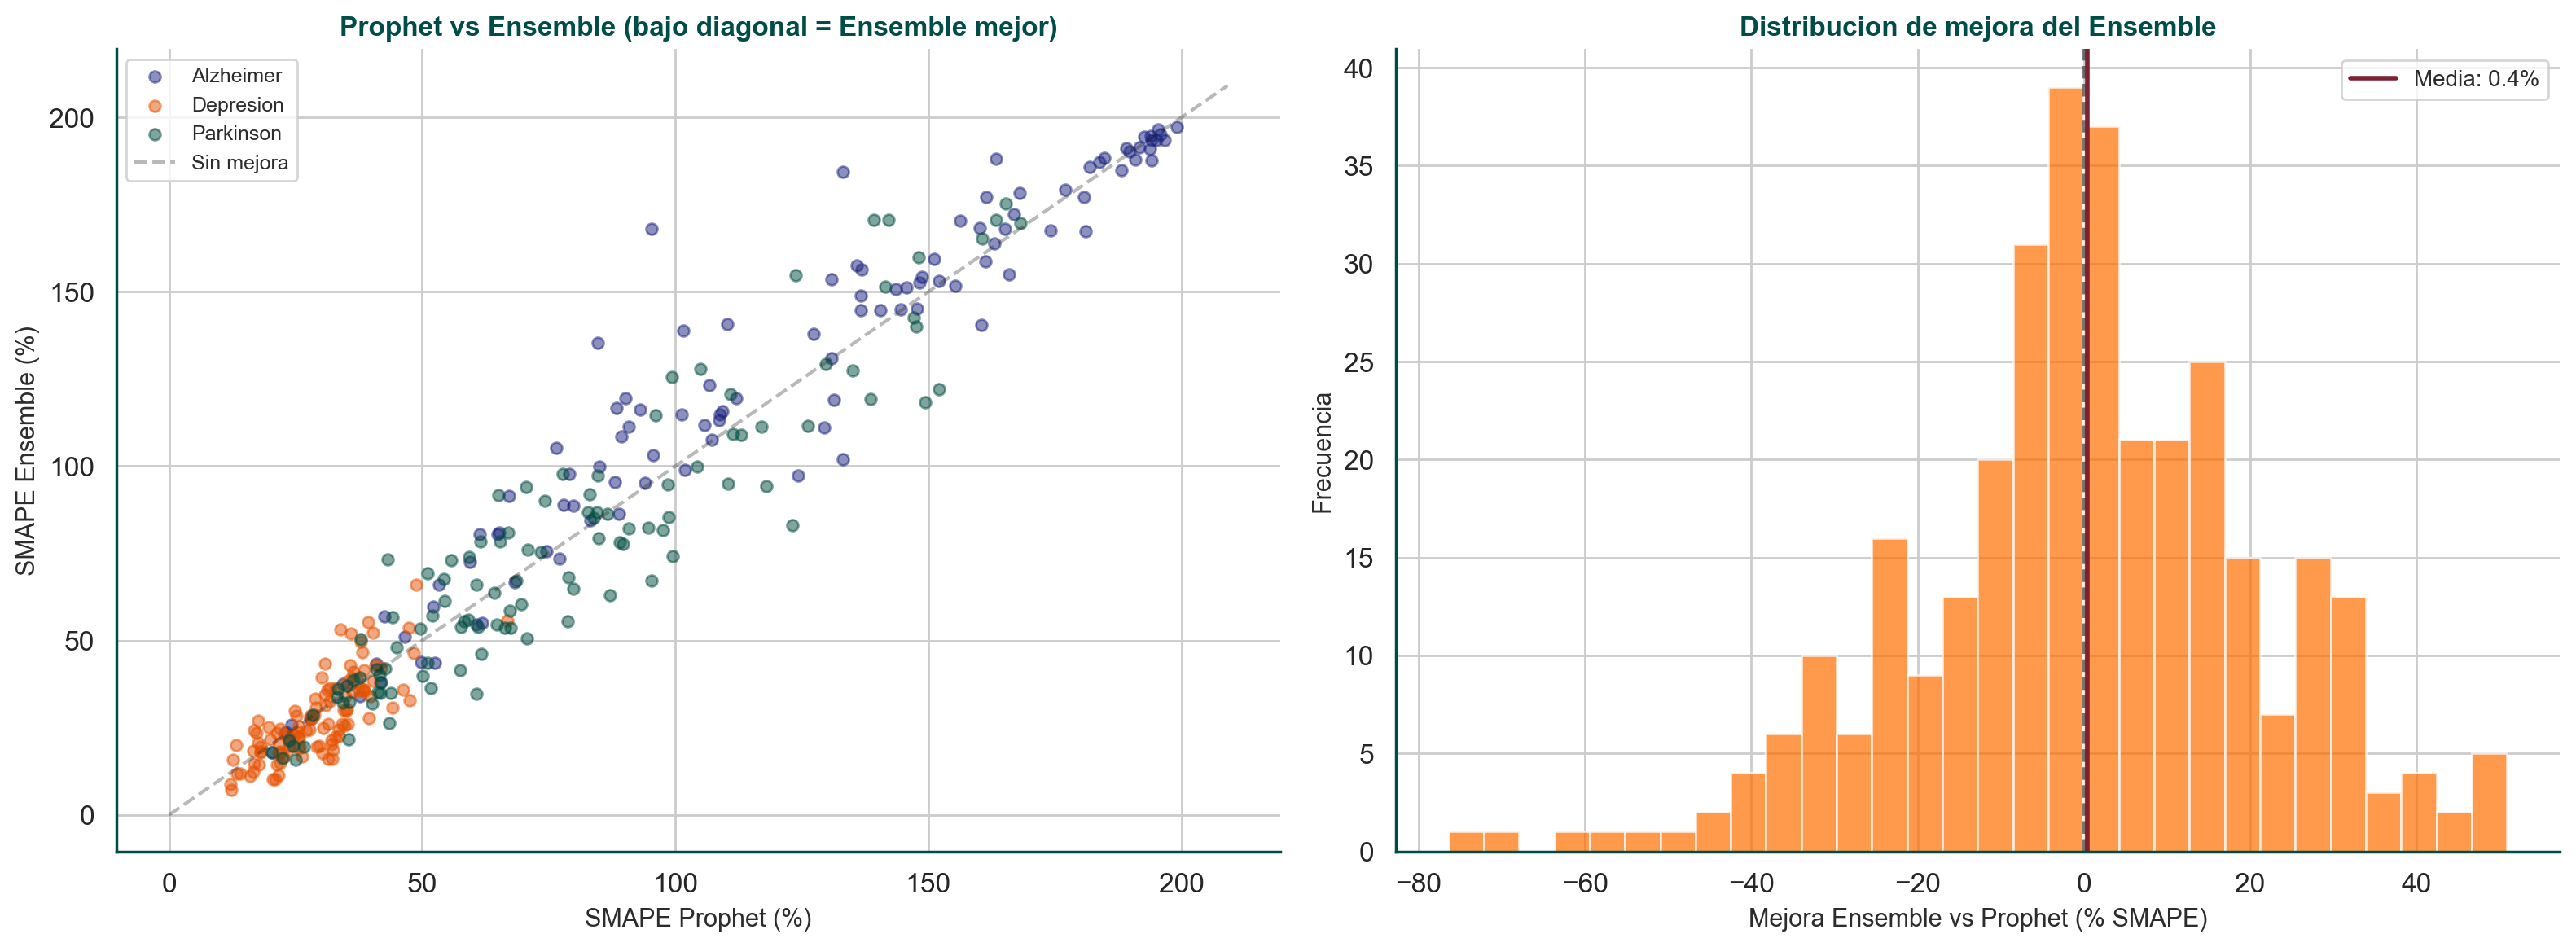
\includegraphics[width=\textwidth]{figuras_avance5/34_mejora_ensemble.png}
        \caption{Mejora porcentual del Ensemble sobre Prophet (baseline).}
        \label{fig:mejora}
    \end{subfigure}
    \caption{Análisis de eficiencia y mejora incremental.}
    \label{fig:eficiencia}
\end{figure}

% ---- FIGURA: Stacked bar producción ----
\begin{figure}[H]
    \centering
    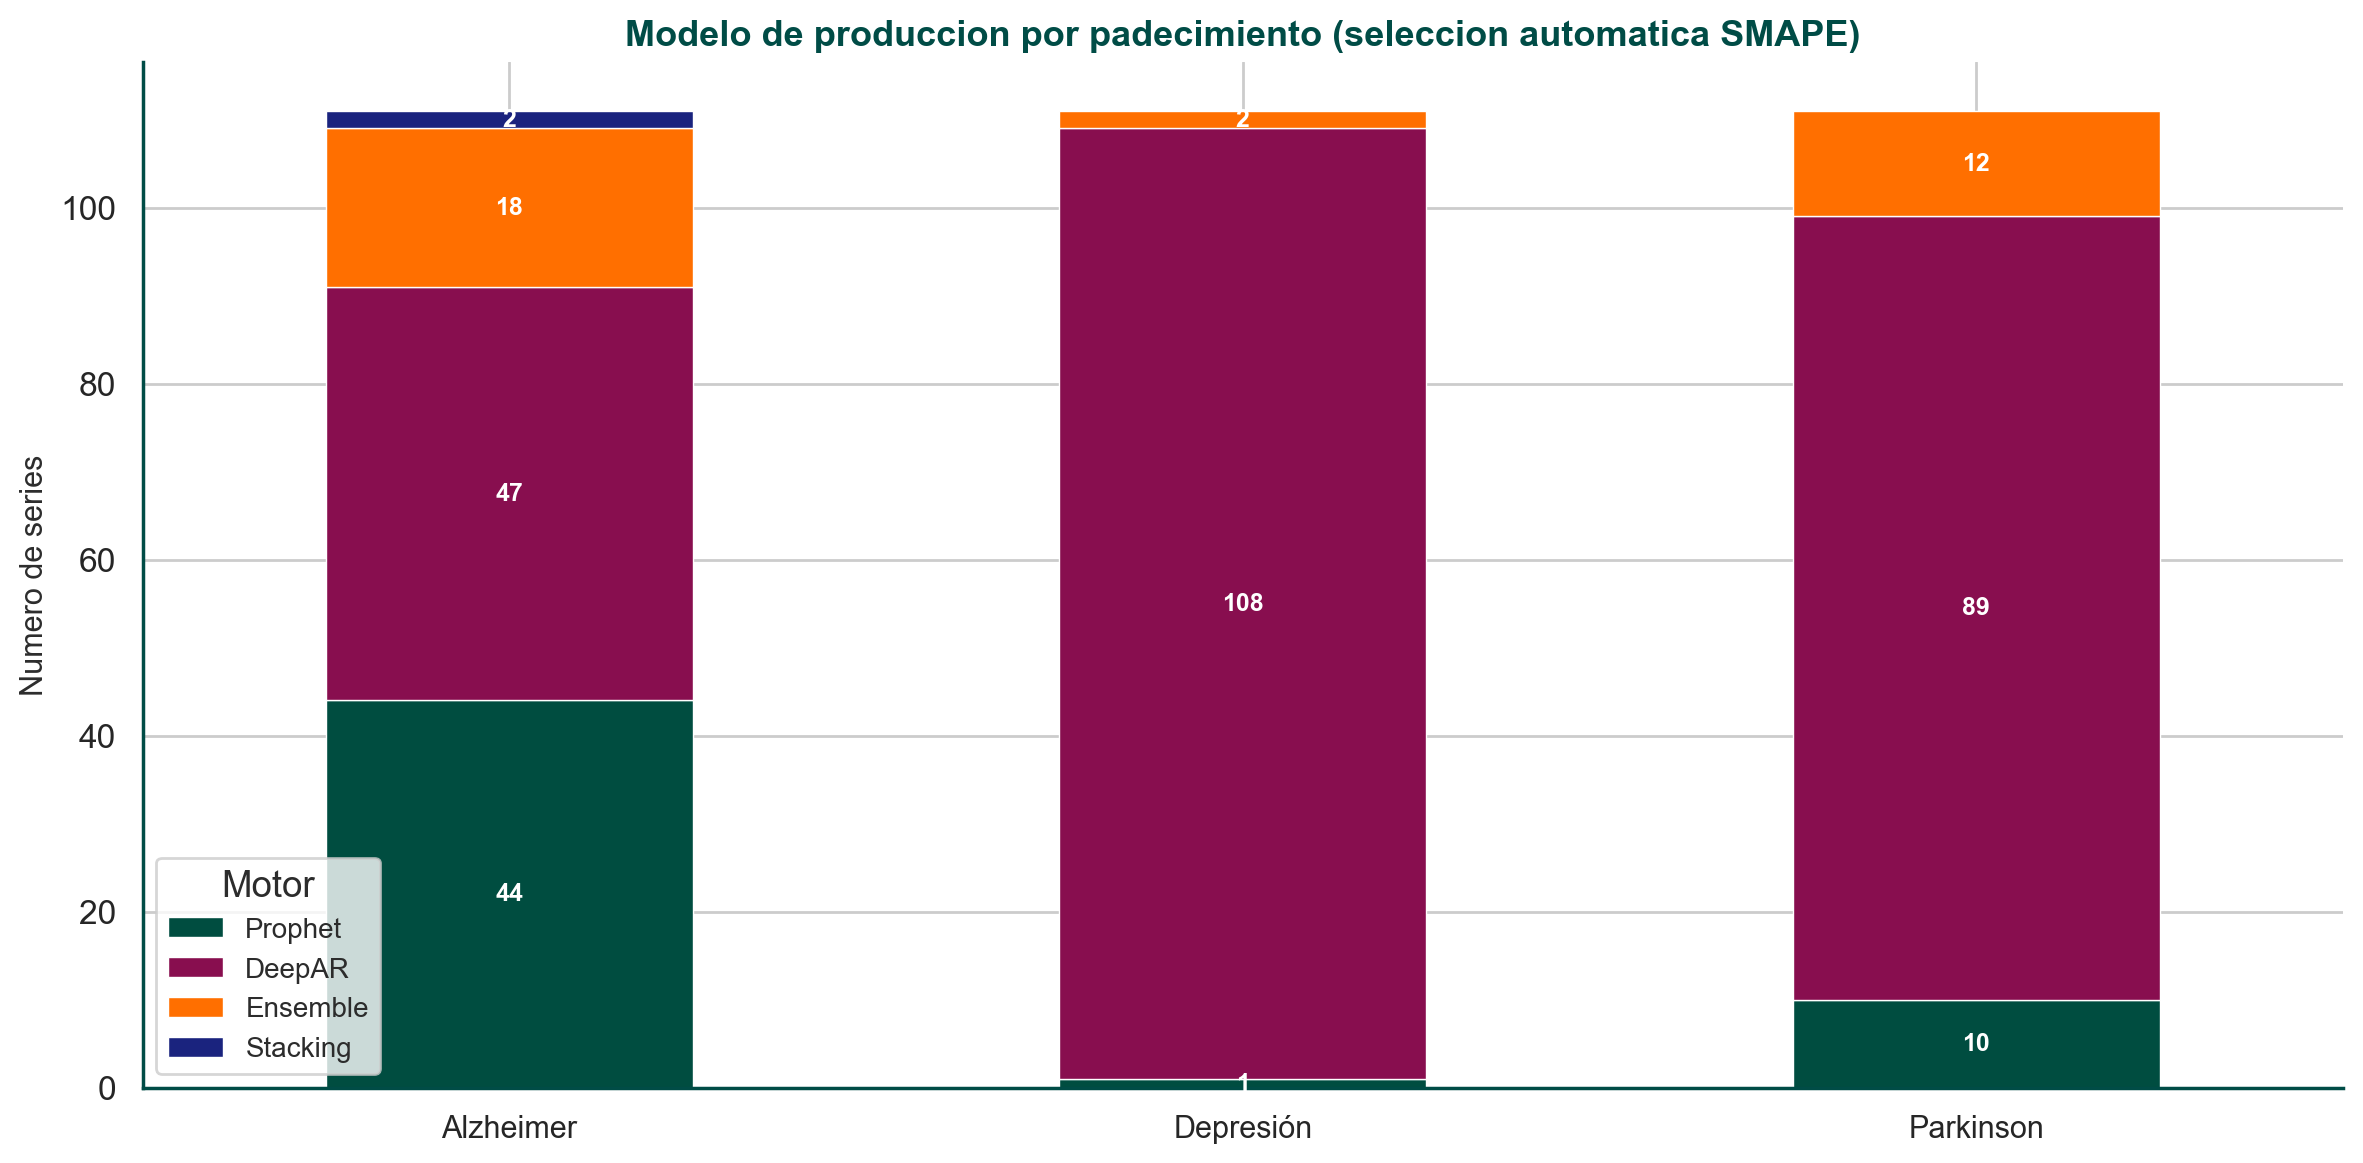
\includegraphics[width=0.80\textwidth]{figuras_avance5/24_stacked_bar_produccion.png}
    \caption{Barras apiladas: distribución del modelo ganador por padecimiento y sexo. DeepAR domina Depresión y Parkinson; Alzheimer muestra competencia cerrada entre DeepAR y Prophet.}
    \label{fig:stacked_bar}
\end{figure}

\newpage

% =============================================================================
% 8. MLOps Y ECOSISTEMA TABLEAU
% =============================================================================
\section{MLOps, Tableau y Arquitectura de Producción}\label{sec:mlops}

\subsection{Pipeline CI/CD y Dashboard}

Se implementó un pipeline CI/CD completo (\texttt{publish\_gsheets.py} vía GitHub Actions) para inyectar pronósticos al Dashboard Ejecutivo en Tableau Public.\footnote{Dashboard disponible en \url{https://proyectointegrador.org/epidashboard}}

\begin{criticalbox}[Optimizador frente al Límite de Google Sheets]
Al generar el forecast de los 1,332 modelos, el dataset superaba los \textbf{120 millones de celdas}, chocando contra el límite estricto de la API de Google Sheets (10 millones).

\textbf{Solución MLOps:} Se construyó un algoritmo de compresión que elimina jerarquías redundantes, reduce el \textit{payload} al 50\,\%, e inyecta los datos en bloques (\textit{chunks}) cada hora sin intervención humana. Se han logrado \textbf{163 ejecuciones exitosas consecutivas}.
\end{criticalbox}

\textbf{Rediseño UI:} Atendiendo la recomendación clínica, el Dashboard se re-estructuró. Los filtros ya no mezclan estados con regiones, y la UI guía al usuario primero por la \textit{Exploración Histórica} antes de mostrar la predicción de \textbf{casos absolutos} para la logística hospitalaria.

% ---- FIGURA: KPI Dashboard ----
\begin{figure}[H]
    \centering
    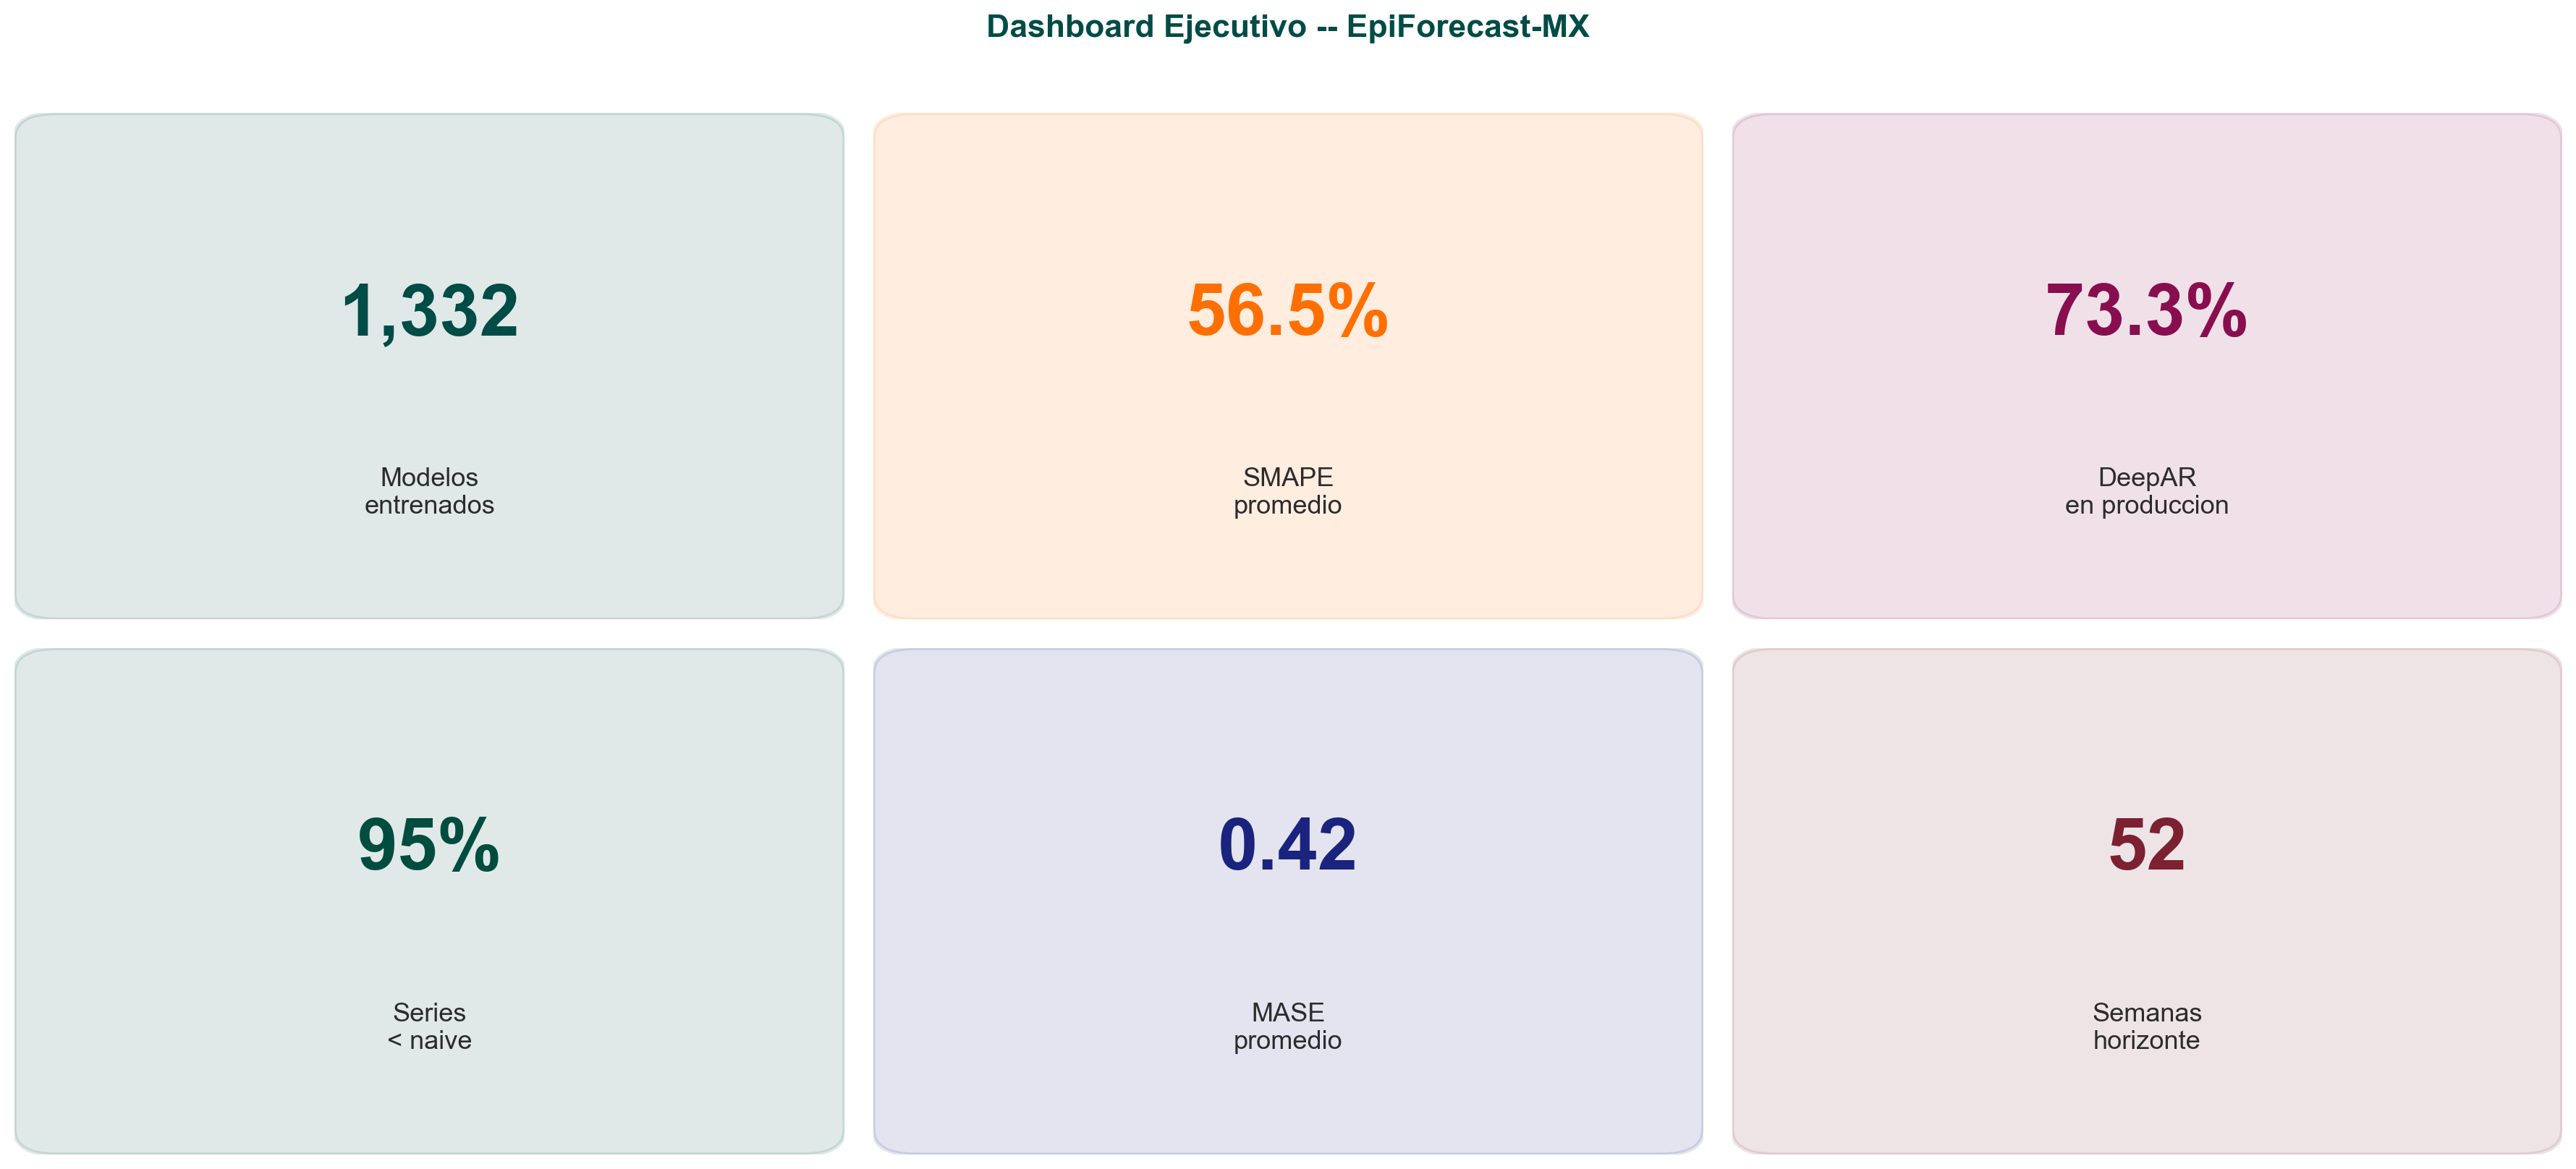
\includegraphics[width=0.9\textwidth]{figuras_avance5/31_kpi_dashboard.png}
    \caption{Panel superior de KPIs ejecutivos de la plataforma EpiForecast-MX en Tableau.}
    \label{fig:kpis}
\end{figure}

\subsection{Infraestructura de Cómputo}

\begin{table}[H]
\centering
\caption{Tiempos de entrenamiento por motor (333 modelos)}
\label{tab:tiempos}
\small
\begin{tabular}{llrr}
\toprule
\textbf{Motor} & \textbf{Hardware} & \textbf{Tiempo total} & \textbf{Promedio/modelo} \\
\midrule
Prophet   & CPU (Apple M3, joblib $-2$) & 7.9 horas  & 85.2 seg \\
DeepAR    & GPU (AWS SageMaker T4)     & 1.5 horas  & N/A (batch) \\
DeepAR    & CPU/MPS (Apple M3 local)   & 4.0 horas  & N/A (batch) \\
Ensemble  & CPU (Apple M3)             & 2.3 horas  & 24.4 seg \\
Stacking  & CPU (Apple M3)             & 1.8 horas  & 19.9 seg \\
\midrule
\textbf{Total (4 motores)} & & \textbf{$\sim$13.5 horas} & \\
\bottomrule
\end{tabular}
\end{table}

\subsection{Artefactos y Versionamiento}

El sistema genera y versiona vía DVC (Data Version Control) conectado a Amazon S3:
\begin{itemize}[noitemsep]
    \item \textbf{1,332 modelos} serializados (\texttt{.pkl}) + \textbf{1,353 CSVs} de forecast.
    \item \textbf{764 pruebas unitarias} (Pytest) con cobertura $>$70\,\%.
    \item \textbf{333 gráficos individuales} del modelo ganador (\texttt{PROD\_MODELS/}).
    \item Pre-commit hooks: Ruff (lint + format), Mypy (tipado estricto), trailing whitespace.
    \item MLflow local para tracking de experimentos (métricas, parámetros, tiempos).
\end{itemize}

\newpage

% =============================================================================
% 9. CONCLUSIONES
% =============================================================================
\section{Conclusiones}\label{sec:conclusiones}

\begin{enumerate}
    \item \textbf{Mejora demostrable:} La introducción de \textit{Ensemble Learning} mitigó las debilidades del modelo base. El Ensemble con XGBoost inyectó reacción a la volatilidad post-COVID, y DeepAR resolvió el ruido en series con ceros mediante \textit{transfer learning}. A nivel global, DeepAR reduce el SMAPE un \textbf{15\,\%} respecto a Prophet (63.13\,\% vs.\ 74.42\,\%).

    \item \textbf{Calidad en datos no vistos:} La reingeniería ética del \textit{backtest} de ventana expansiva garantizó métricas honestas. La eliminación de dos fuentes de \textit{data leakage} (en preprocesamiento y en features del Ensemble) y la implementación de 764 tests automatizados aseguran la integridad del pipeline.

    \item \textbf{El paradigma Multi-motor:} No existe un algoritmo universal. DeepAR domina el 73.3\,\% de las series (nivel micro), mientras que Ensemble y Prophet prevalecen en agregados macro y series de bajo volumen, respectivamente. El enrutador dinámico asigna el mejor motor para cada una de las 333 combinaciones clínicas.

    \item \textbf{Robustez clínica:} El 98.5\,\% de los modelos de producción presentan overfitting controlado ($<1.3\times$) y el 99.1\,\% está libre de sospecha de leakage. Las 8 series con incidencia insuficiente se reasignan automáticamente a su modelo regional.

    \item \textbf{Pronósticos accionables:} El sistema proyecta \textbf{451,571 casos de Depresión}, \textbf{23,775 de Parkinson} y \textbf{7,212 de Alzheimer} para las próximas 52 semanas, información que permite al IMSS planificar camas, insumos y personal con anticipación.
\end{enumerate}

\newpage

% =============================================================================
% 10. REFLEXIONES PERSONALES DEL EQUIPO
% =============================================================================
\section{Reflexiones Personales del Equipo}\label{sec:reflexiones}

\begin{minipage}[t]{0.18\textwidth}
    \vspace{0pt}
    
\includegraphics[width=\linewidth, clip, trim=0 0 0 0]{JARS2026.jpg}
\end{minipage}%
\hfill
\begin{minipage}[t]{0.78\textwidth}
    \vspace{0pt}
    \textbf{Javier Augusto Rebull Saucedo} \\
    \textit{\small Sr.\ Associate Development Application, Santander Bank US}

    \smallskip
    El paso hacia Ensemble Learning redefinió el concepto de escalabilidad en nuestro sistema. Descubrir que DeepAR domina a nivel estatal pero pierde contra XGBoost a nivel Nacional me enseñó el valor del diseño MLOps. Construir un enrutador inteligente que selecciona dinámicamente entre 4 motores basándose en el SMAPE de prueba fue el reto de ingeniería más satisfactorio. La detección de \textit{data leakage} en el feature builder nos obligó a repensar cada supuesto: una lección que aplico ahora en mi trabajo diario en banca.
\end{minipage}

\vspace{0.8cm}

\begin{minipage}[t]{0.18\textwidth}
    \vspace{0pt}
    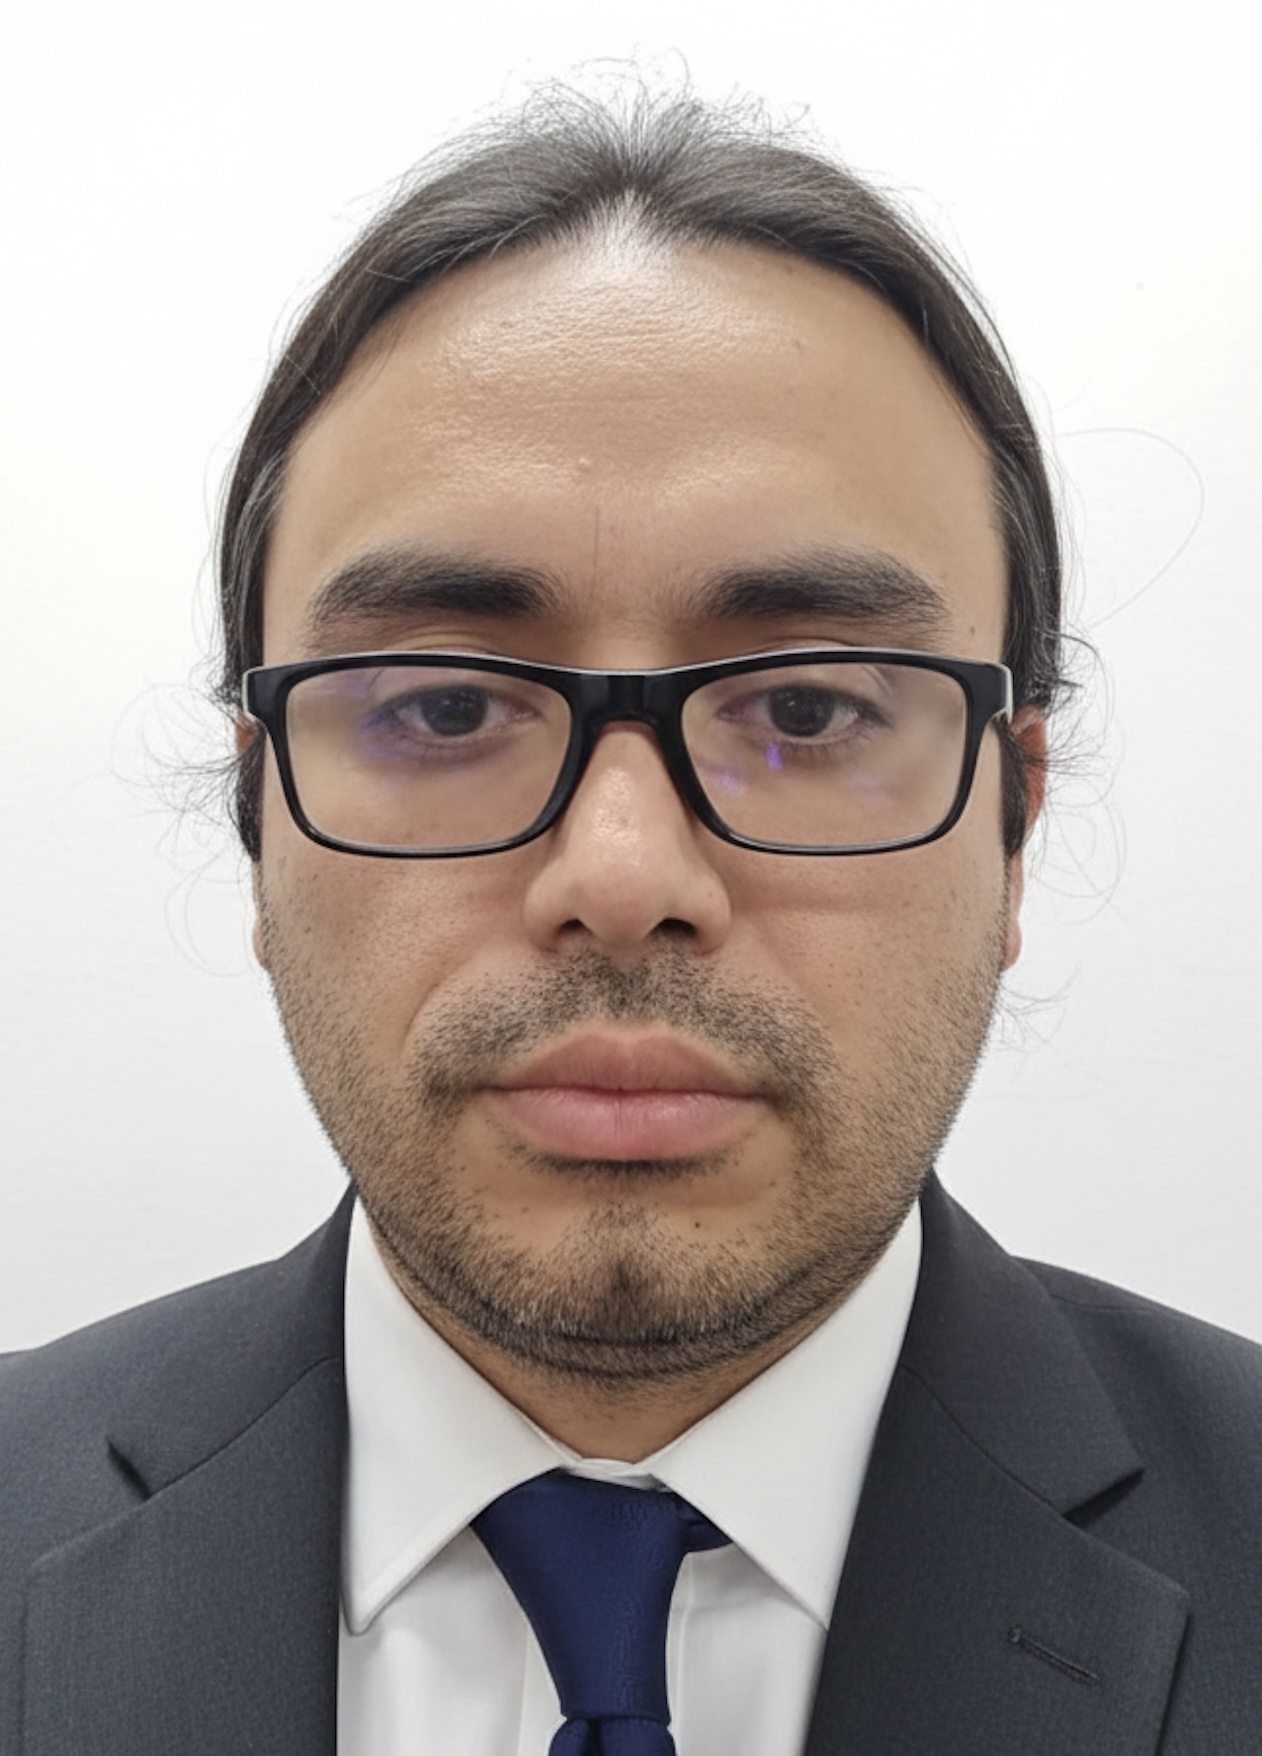
\includegraphics[width=\linewidth, clip, trim=0 0 0 0]{JARCOS2026.jpg}
\end{minipage}%
\hfill
\begin{minipage}[t]{0.78\textwidth}
    \vspace{0pt}
    \textbf{Juan Carlos Pérez Nava} \\
    \textit{\small Head of Area, Instituto Mexicano del Seguro Social (IMSS)}

    \smallskip
    Validar que el modelo traduzca matemáticas (tasas por 100k) en \textbf{casos absolutos} en el Dashboard cerró el círculo con el negocio. El IMSS planea con pacientes reales, no con coeficientes. Ver cómo XGBoost y DeepAR corrigieron la suavidad excesiva de Prophet me demostró que confiar en la diversidad algorítmica convierte un ejercicio académico en una herramienta de salud pública. El fallback regional para series de ceros fue un diseño que nació de la necesidad clínica real: no podemos dejar estados sin pronóstico solo porque su incidencia histórica es mínima.
\end{minipage}

\vspace{0.8cm}

\begin{minipage}[t]{0.18\textwidth}
    \vspace{0pt}
    
\includegraphics[width=\linewidth, clip, trim=0 0 0 0]{LUIS2026.jpg}
\end{minipage}%
\hfill
\begin{minipage}[t]{0.78\textwidth}
    \vspace{0pt}
    \textbf{Luis Gerardo Sánchez Salazar} \\
    \textit{\small Sr.\ Controls Engineer, Tesla}

    \smallskip
    La topología del Stacking resonó con mi formación en ingeniería de controles: un \textit{meta-learner} actuando como un controlador PID que ajusta pesos dinámicamente según la época del año. Sin embargo, mi mayor contribución fue llevar los resultados al terreno visual a través de \textbf{Tableau Public}. Construir el dashboard epidemiológico implicó retos que no anticipé: transformar 333 pronósticos semanales en vistas interactivas que un epidemiólogo del IMSS pudiera interpretar sin formación en ciencia de datos. El filtrado dinámico por entidad, padecimiento y sexo requirió múltiples iteraciones de diseño UX; la desnormalización de tasas a casos absolutos generó discrepancias que tuvimos que reconciliar entre el pipeline de Python y las fórmulas calculadas de Tableau. El mayor desafío fue la actualización semanal: automatizar la ingesta de nuevos boletines, regenerar los CSVs y publicar sin romper los enlaces compartidos con el IMSS. Hoy el dashboard es la cara visible del proyecto, y la lección fue clara: un modelo que nadie puede visualizar es un modelo que nadie usa.
\end{minipage}

\newpage

% =============================================================================
% REFERENCIAS
% =============================================================================
\section*{Referencias}
\addcontentsline{toc}{section}{Referencias}

\begin{enumerate}[label={[\arabic*]}, leftmargin=*, noitemsep]
    \item Singh, A. (2023). Comprehensive Guide to Ensemble Learning. \textit{Analytics Vidhya}.

    \item VanderPlas, J. (2022). Thinking About Model Validation. En \textit{Python Data Science Handbook} (2a ed., pp.~410--427). O'Reilly Media.

    \item Salinas, D., Flunkert, V., Gasthaus, J. \& Januschowski, T. (2020). DeepAR: Probabilistic forecasting with autoregressive recurrent networks. \textit{International Journal of Forecasting}, 36(3), 1181--1191.

    \item Taylor, S.\,J. \& Letham, B. (2018). Forecasting at scale. \textit{The American Statistician}, 72(1), 37--45.

    \item Chen, T. \& Guestrin, C. (2016). XGBoost: A Scalable Tree Boosting System. En \textit{Proc.\ 22nd ACM SIGKDD} (pp.~785--794).

    \item Makridakis, S. (1993). Accuracy measures: theoretical and practical concerns. \textit{International Journal of Forecasting}, 9(4), 527--529.

    \item Hyndman, R.\,J. \& Koehler, A.\,B. (2006). Another look at measures of forecast accuracy. \textit{International Journal of Forecasting}, 22(4), 679--688.

    \item Ke, G., Meng, Q., Finley, T. et al. (2017). LightGBM: A Highly Efficient Gradient Boosting Decision Tree. \textit{Advances in Neural Information Processing Systems}, 30.

    \item Zou, H. \& Hastie, T. (2005). Regularization and variable selection via the elastic net. \textit{Journal of the Royal Statistical Society B}, 67(2), 301--320.

    \item Hyndman, R.\,J., Koehler, A.\,B., Snyder, R.\,D. \& Grose, S. (2002). A state space framework for automatic forecasting using exponential smoothing methods. \textit{International Journal of Forecasting}, 18(3), 439--454.
\end{enumerate}

\newpage


% =============================================================================
% APÉNDICE B: GLOSARIO DE TÉRMINOS PARA PÚBLICO NO TÉCNICO
% =============================================================================
\newpage
\section*{Apéndice: Glosario de Términos}
\addcontentsline{toc}{section}{Apéndice: Glosario de Términos}

El siguiente glosario explica los términos técnicos utilizados en este documento, con el objetivo de que profesionales de la salud, tomadores de decisión y público general puedan interpretar los resultados sin necesidad de formación en ciencia de datos.

\begin{longtable}{>{\bfseries\small}p{3.8cm} p{11.5cm}}
\toprule
\textbf{Término} & \textbf{Significado} \\
\midrule
\endfirsthead
\multicolumn{2}{c}{\small\textit{(continuación del Glosario)}} \\
\toprule
\textbf{Término} & \textbf{Significado} \\
\midrule
\endhead
\midrule
\multicolumn{2}{r}{\small\textit{Continúa en la siguiente página}} \\
\endfoot
\bottomrule
\endlastfoot

Backtest & Simulación retrospectiva: se ``esconde'' parte de los datos históricos y se evalúa si el modelo habría acertado, como un examen sorpresa hacia el pasado. \\
\addlinespace
Baseline & Modelo de referencia o punto de partida. Es el primer modelo simple con el que se comparan todos los demás para medir si realmente mejoran. \\
\addlinespace
Boosting & Técnica donde varios modelos simples se entrenan de forma secuencial; cada uno intenta corregir los errores que dejó el anterior, como un equipo de relevos donde cada corredor aprende del tropiezo del compañero previo. \\
\addlinespace
Changepoint & Punto en el tiempo donde la tendencia de los datos cambia de dirección (por ejemplo, el inicio de la pandemia COVID-19). \\
\addlinespace
CIE-10 & Clasificación Internacional de Enfermedades, 10.ª revisión. Catálogo mundial que asigna un código a cada enfermedad (F32 = Depresión, G20 = Parkinson, G30 = Alzheimer). \\
\addlinespace
Cold Start & ``Arranque en frío'': cuando un modelo no tiene suficientes datos históricos para aprender patrones confiables, como intentar predecir el clima de un lugar donde apenas se instaló la estación meteorológica. \\
\addlinespace
Cross-Validation & Validación cruzada: dividir los datos en partes, entrenar con unas y evaluar con otras, para asegurarse de que el modelo funciona con datos que nunca ha visto. \\
\addlinespace
Data Leakage & Fuga de datos: error donde el modelo ``espía'' información del futuro durante el entrenamiento, produciendo resultados artificialmente buenos que no se sostienen en la realidad. \\
\addlinespace
DeepAR & Modelo de inteligencia artificial basado en redes neuronales (LSTM) que aprende patrones de múltiples series de datos simultáneamente, permitiéndole ``pedir prestada'' información de unos estados para mejorar las predicciones de otros. \\
\addlinespace
Desagregación & Separar los datos por categorías (en este caso: por estado y por sexo) en lugar de analizarlos todos juntos, para detectar patrones específicos de cada grupo. \\
\addlinespace
DVC & Data Version Control: herramienta que registra cada versión de los datos y modelos, similar a un sistema de control de versiones para documentos pero diseñado para archivos grandes de datos. \\
\addlinespace
ElasticNet & Modelo estadístico que combina dos tipos de regularización (penalización) para evitar que el modelo se ``descontrole'' al trabajar con datos ruidosos o incompletos. \\
\addlinespace
Ensemble Learning & Aprendizaje por ensamble: combinar las predicciones de varios modelos diferentes para obtener una respuesta más confiable, similar a consultar la opinión de varios especialistas antes de tomar una decisión médica. \\
\addlinespace
Entidad Federativa & Cada uno de los 32 estados que componen México. \\
\addlinespace
Estacionalidad & Patrones que se repiten de forma cíclica (por ejemplo, la depresión suele aumentar en ciertas épocas del año). \\
\addlinespace
ETS (Holt-Winters) & Modelo estadístico clásico que descompone una serie de tiempo en tres componentes: nivel, tendencia y estacionalidad. \\
\addlinespace
Fallback Regional & Modelo de respaldo: cuando un estado tiene muy pocos casos para hacer predicciones confiables, se usa el modelo de su región geográfica (que tiene más datos) como sustituto. \\
\addlinespace
Feature & Variable o dato que el modelo usa para hacer predicciones (por ejemplo, ``casos de hace un año'' o ``¿estábamos en pandemia?''). \\
\addlinespace
Feature Importance & Importancia de características: ranking que indica cuáles variables son más útiles para que el modelo haga predicciones precisas. \\
\addlinespace
Fold & Cada una de las particiones de datos que se utilizan en la validación cruzada. Si se usan 4 folds, los datos se dividen en 4 partes. \\
\addlinespace
Forecast & Pronóstico: la predicción numérica de cuántos casos se esperan en el futuro. \\
\addlinespace
Fourier (series de) & Herramienta matemática que descompone patrones cíclicos en ondas simples, permitiendo al modelo capturar estacionalidades complejas. \\
\addlinespace
Grid Search & Búsqueda exhaustiva: probar todas las combinaciones posibles de configuraciones del modelo para encontrar la que funciona mejor. \\
\addlinespace
Hiperparámetro & Configuración que el humano ajusta antes de entrenar el modelo (análogo a los ``diales'' de una máquina que se calibran antes de encenderla). \\
\addlinespace
Horizonte de predicción & Qué tan lejos en el futuro se predicen los datos. En EpiForecast-MX el horizonte es de 52 semanas (un año). \\
\addlinespace
Incidencia & Número de casos nuevos de una enfermedad en un periodo y población determinados. \\
\addlinespace
INEGI & Instituto Nacional de Estadística y Geografía: organismo que provee las proyecciones de población usadas para calcular tasas. \\
\addlinespace
LightGBM & Variante eficiente de Gradient Boosting (árboles de decisión potenciados) desarrollada por Microsoft, optimizada para velocidad con grandes volúmenes de datos. \\
\addlinespace
LSTM & \textit{Long Short-Term Memory}: tipo de red neuronal especialmente diseñada para aprender patrones en secuencias de datos (como series semanales de casos). \\
\addlinespace
MAE & Error Absoluto Medio: promedio de las diferencias (sin signo) entre lo que el modelo predijo y lo que realmente pasó. Más bajo es mejor. \\
\addlinespace
MASE & Error Escalado Absoluto Medio: compara el error del modelo contra una predicción ``ingenua'' (repetir el último valor conocido). Si MASE $< 1.0$, el modelo es mejor que simplemente repetir el pasado. \\
\addlinespace
Meta-learner & Modelo ``árbitro'' que aprende a combinar las predicciones de otros modelos, decidiendo cuánto confiar en cada uno. \\
\addlinespace
MLOps & Conjunto de prácticas de ingeniería para poner modelos de inteligencia artificial en producción de forma confiable, reproducible y automatizada. \\
\addlinespace
Monte Carlo (muestras) & Técnica que genera múltiples escenarios aleatorios para estimar la incertidumbre de las predicciones (como lanzar muchos dados para calcular probabilidades). \\
\addlinespace
Out-of-Fold (OOF) & Predicciones generadas sobre datos que el modelo no vio durante su entrenamiento, garantizando una evaluación honesta. \\
\addlinespace
Overfitting & Sobreajuste: cuando el modelo ``memoriza'' los datos de entrenamiento en lugar de aprender patrones generales, produciendo buenos resultados históricos pero malas predicciones futuras. \\
\addlinespace
Pipeline & Secuencia automatizada de pasos que van desde los datos crudos hasta las predicciones finales, como una línea de ensamblaje digital. \\
\addlinespace
Prophet & Modelo de pronóstico creado por Meta (Facebook) que descompone una serie de tiempo en tendencia, estacionalidad y eventos especiales (como días festivos o pandemias). \\
\addlinespace
Ridge (regresión) & Modelo estadístico que añade una penalización para evitar pesos extremos, obligando al modelo a distribuir la importancia de forma equilibrada entre sus componentes. \\
\addlinespace
RMSE & Raíz del Error Cuadrático Medio: similar al MAE pero penaliza más los errores grandes. Más bajo es mejor. \\
\addlinespace
Serie de Tiempo & Secuencia de datos registrados a intervalos regulares en el tiempo (en nuestro caso, casos semanales de cada enfermedad). \\
\addlinespace
SINAVE & Sistema Nacional de Vigilancia Epidemiológica: la red oficial de México que recopila y publica datos de enfermedades a través de boletines semanales. \\
\addlinespace
SMAPE & Error Porcentual Absoluto Medio Simétrico: mide qué tan lejos estuvo la predicción del valor real, expresado como porcentaje. Un SMAPE de 10\,\% significa que la predicción se desvió en promedio un 10\,\% del valor observado. \\
\addlinespace
Stacking & Apilamiento: técnica avanzada de ensamble donde un modelo supervisor aprende a combinar las salidas de múltiples modelos base, ponderando la confianza en cada uno según el contexto. \\
\addlinespace
Tasa por 100k hab. & Número de casos por cada 100,000 personas. Permite comparar estados con poblaciones muy diferentes (p.~ej., Estado de México vs.\ Colima). \\
\addlinespace
Transfer Learning & Aprendizaje por transferencia: usar el conocimiento adquirido al analizar un conjunto de datos (p.~ej., un estado grande) para mejorar las predicciones en otro con menos información. \\
\addlinespace
Ventana Expansiva & Método de evaluación donde el periodo de entrenamiento crece progresivamente, simulando cómo el modelo habría funcionado en la vida real mes a mes. \\
\addlinespace
XGBoost & Algoritmo de aprendizaje automático basado en árboles de decisión potenciados, muy eficaz para detectar patrones complejos en datos tabulares. \\
\end{longtable}


\end{document}
